
\documentclass[doublespacing]{brandeis}
%\documentclass[doublespacing, draft]{brandeis}
\usepackage{bm}
\usepackage{url}
\usepackage{tikz}
\usepackage{soul}
\usepackage{color}
\usepackage{times}
\usepackage{dsfont}
\usepackage{pifont}
%\usepackage{breqn}
\usepackage{textcomp}
\usepackage{wrapfig}
\usepackage{graphicx}
\usepackage{multirow}
\usepackage{multicol}
\usepackage{footnote}
\usepackage{pgfplots}
\usepackage{verbatim}
\usepackage{textcomp}
\usepackage{booktabs}
\usepackage{textcomp}
\usepackage{paralist}
\usepackage{algorithm}
\usepackage{algpseudocode}
\usepackage[makeroom]{cancel}
\algrenewcommand\textproc{} % to change function names to lower case
\usepackage{mathrsfs}
\usepackage{microtype}
\usepackage{schemabloc}
\usepackage{algpseudocode}
\usepackage[final]{pdfpages}
\usepackage[export]{adjustbox}
% Optional: If your LaTeX has microtype, use it to improve text quality:
%\usepackage{microtype}
\usepackage[most]{tcolorbox}
\usepackage{booktabs,tabularx}
\usepackage{caption}
\usepackage[T1]{fontenc}

\captionsetup[table]{skip=4pt,singlelinecheck=off}

% correct bad hyphenation here
\hyphenation{op-tical net-works semi-conduc-tor}

% Recommended: If your dissertation contains math, use the AMS packages:
\usepackage{amsmath}
\numberwithin{equation}{section}
\usepackage{amssymb,amsthm}
\usepackage[caption=false,font=normalsize,labelfont=sf,textfont=sf]{subfig}
%
\let\proof\relax
\let\endproof\relax
\usepackage[final]{pdfpages}


%\addtolength{\textfloatsep}{-5mm}
\addtolength{\textfloatsep}{-3mm}
\pgfplotsset{compat=1.5}

% Required: To satisfy UTD's formatting requirements for citations, use the
% "natbib" package.  (Use other citation packages at your own risk; not all
% are flexible enough to meet UTD's requirements.)  If you wish to use numeric
% citations, change "authoryear" to "numbers" below.  Use the "chicago" BibTeX
% style, which most closely matches the Turabian formatting required by UTD.
% UTD mandates a blank line between each pair of bibliography entries, so set
% \bibsep as shown below.  Finally, if you are accustomed to using \cite as
% your citation macro, point it to natbib's \citep macro as shown.
\usepackage[authoryear, sort]{natbib}
\bibliographystyle{chicago}
\setlength{\bibsep}{12pt plus 1pt minus 1pt}
\let\cite=\citep
\usepackage{rotating}
%\theoremstyle{remark}

\theoremstyle{definition}
\newtheorem{definition}{Definition}[]
\newtheorem{example}{Example}[]
\newtheorem{quiz}{Quiz}
\newtheorem{homework}{Homework}
%\usepackage[pagebackref=true,breaklinks=true,bookmarks=true]{hyperref}
\usepackage[pagebackref=true,breaklinks=true,colorlinks=true, citecolor=green,linkcolor=light-blue,urlcolor=blue,bookmarks=true]{hyperref}
%%% End of packages.
% Define all your personal macros here (if you have any).
%
\definecolor{light-blue}{rgb}{0.30,0.35,1}
\definecolor{light-green}{rgb}{0.20,0.49,.85}
\definecolor{purple}{rgb}{0.70,0.69,.2}

\newcommand{\lb}[1]{\textcolor{light-blue}{#1}}
\newcommand{\bl}[1]{\textcolor{blue}{#1}}

\newcommand{\maybe}[1]{\textcolor{gray}{\textbf{MAYBE: }{#1}}}
\newcommand{\inspect}[1]{\textcolor{cyan}{\textbf{CHECK THIS: }{#1}}}
\newcommand{\more}[1]{\textcolor{red}{\textbf{MORE: }{#1}}}

% FYA
\newcommand{\cmt}[1]{{\footnotesize\textcolor{red}{#1}}}%{#2}
%\newcommand{\note}[1]{\cmt{Note: #1}}
%\newcommand{\todo}[1]{\textcolor{cyan}{TO-DO: #1}}
\newcommand{\review}[1]{\noindent\textcolor{red}{$\rightarrow$ #1}}
\newcommand{\response}[1]{\noindent{#1}}
\newcommand{\stopped}[1]{\color{red}STOPPED HERE #1\hrulefill}

%Text commands
\newcounter{mnote}
\newcommand{\marginote}[1]{\addtocounter{mnote}{1}\marginpar{\themnote. \scriptsize #1}}
\setcounter{mnote}{0}
% \newcommand{\comment}[1]{}
\newcommand{\ie}{$i.e.$\ }
\newcommand{\eg}{e.g.\ }
\newcommand{\cf}{c.f.\ }
\newcommand{\yes}{\checkmark}
\newcommand{\no}{\ding{55}}

%Reference commands
\newcommand{\flabel}[1]{\label{fig:#1}}
\newcommand{\seclabel}[1]{\label{sec:#1}}
\newcommand{\tlabel}[1]{\label{tab:#1}}
\newcommand{\elabel}[1]{\label{eq:#1}}
\newcommand{\alabel}[1]{\label{alg:#1}}
\newcommand{\fref}[1]{\cref{fig:#1}}
\newcommand{\sref}[1]{\cref{sec:#1}}
\newcommand{\tref}[1]{\cref{tab:#1}}
\newcommand{\eref}[1]{\cref{eq:#1}}
\newcommand{\aref}[1]{\cref{alg:#1}}

\newcommand{\bull}[1]{$\bullet$ #1}
\newcommand{\argmax}{\text{argmax}}
\newcommand{\argmin}{\text{argmin}}
\newcommand{\mc}[1]{\mathcal{#1}}
\newcommand{\bb}[1]{\mathbb{#1}}


\def\tidx{t}
%\def\comment
%\def\value{V}
% from https://www.cs.jhu.edu/~jason/advice/write-the-paper-first.html
\newcommand{\Note}[1]{}
\renewcommand{\Note}[1]{\hl{[#1]}}  % comment out this definition to suppress all Notes
%\algnewcommand\algorithmicforeach{\textbf{for each}}
%\algdef{S}[FOR]{Foreach}[1]{\algorithmicforeach\ #1\ \algorithmicdo} %

%\newcolumntype{M}[1]{>{\centering\arraybackslash}m{#1}}
\def\coriolis{\textbf{\textit{C}}}
\def\massinertia{\textbf{\textit{M}}}
\def\torque{\bm{\tau}}
\def\frictionvec{\textbf{\textit{f}}}
\def\Smat{\textbf{\textit{S}}}
\def\Bmat{\textbf{\textit{B}}}
\def\wheelrad{\textbf{\textit{r}}}

\def\stateweight{\textbf{\textit{w}}_x}
\def\actionweight{\textbf{\textit{w}}_u}
\def\advactionweight{\textbf{\textit{w}}_v}

%Thesis defs
%\def\upchi{\textchi}
\def\kau{\mc{K}}
\def\particle{\bm{x}}
\def\deformationgrad{\textbf{F}}
\def\refconf{\bm{\upchi}_0}
\def\refconfbody{\mathscr{B}_0}
\def\conf{\bm{\upchi}}
\def\currconf{\bm{\upchi}}
\def\Eulerian{\mc{E}}
\def\cauchystress{\bm{\sigma}}
\def\stresscomp{\sigma}
\def\currconfbody{\mathscr{B}}
\def\materialresponse{\textbf{G}}
\def\orthoggroup{{\textit{SO}}(3)}
\def\liegroup{{\textit{SE}}(3)}
\def\liealgebra{\mathfrak{se}(3)}
\def\identity{\textbf{I}}
\newcommand{\trace}[1]{\textbf{tr}(#1)}
\def\leftcauchy{\textbf{B}}
\def\rightcauchy{\textbf{C}}
\def\fiber{\textbf{dx}}

\def\dof{\text{DOF }}
\def\dofs{\text{DOFs }}
\def\reline{\mathbb{R}}
\def\curve{\deformationgrad}
\def\twist{{\xi}}
\def\contactforce{\tilde{F}}
\def\contactforcecomp{f}
\def\gaussianmap{\textbf{}n}
\def\contacttorquecomp{\tau}
\def\wrt{with respect to }
\def\curveparam{\position}
\def\basis{\bm{e}}
\def\pose{{g}}
\def\selmap{{B}}
\def\manipmap{{G}}
\def\jacob{\bm{J}}
\def\normal{\bm{n}}
\def\position{\textbf{r}}
\def\deformationgradcur{\textbf{H}}
\def\eulerianvel{\textbf{v}(\position, t)}
\def\headparam{\zeta}
\def\strain{\mathrm{\Psi}}
\def\strainiso{\mathrm{\Psi_{\text{iso}}}}
\def\strainfiber{\mathrm{\Psi_{\text{mesh}}}}

% mechanism defs
\def\wallthickness{1cm}
\def\sorodiam{9 cm}
\def\sorodiamdim{5-6.25cm}

% inline macros
\newcommand{\putsoro}[2]{\includegraphics[width=.45\columnwidth,height=#2\columnwidth]{../../../PhDThesis/figures/#1}}
\newcommand{\sorowidth}{.35}


%\newtheorem{theorem}{Theorem}[]
%\newtheorem{example}{Example}
%\newtheorem{homework}{Homework}

\providecommand{\hyperref}[2][]{#2}

\newenvironment{exampleclasscode}
{\parindent=1cm\vskip0pt plus2pt minus0pt\begin{verse}}
	{\end{verse}\vskip0pt plus2pt minus0pt}
%
%%% End of personal macro definitions.
%%% The following definitionhttps://raw.githubusercontent.com/lakehanne/BrandeisNotes/master/lec_notes/def.tex?token=ACAKCJEHYDW72GOQJBSXI3K6GXPIMs MUST come before the document begins.
%
\author{RBOT101: Mathematical Foundations of  Robotics \\
	Instructor: Dr. Lekan Molu}
\title{RBOT 101: Mathematical Foundations of  Robotics.
}

%\pdfoutput=1    % for arxiv tex processor
\begin{document}	
	\frontmatter
	
	%\signaturepage
	\copyrightpage{2021} % optional
	
	\tableofcontents
	\listoffigures % required if you have any figures
	\listoftables % required if you have any tables
	
	\mainmatter
%%
\newpage
%\chapter{Preamble}
\label{chap:intro}

Consider this your roadmap for the course.  Please read through the syllabus posted on moodle carefully and feel free to share any questions that you may have.  Please print a copy of the syllabus for reference. Some relevant parts of the syllabus are repeated here but the moodle reference should serve as your guide throughout the ten weeks of this course.

\section{Course Description}
This course focuses on the algorithmic and mathematical concepts  with respect to robot planning, manipulation and control. Topics covered include kinematics and dynamics, as well as path planning and deep reinforcement learning algorithms. Simulations and experiments on hardware testbeds (listed in the syllabus) will be performed to test the related algorithms.

\section{Course Outcomes}
After taking this course, each student will be able to

\begin{itemize}
\item Develop planning and manipulation schemes to drive robot operation

\item Integrate perception algorithms into manipulation and planning systems

\item Determine the kinematic description of a robot's motion or locomotion
\end{itemize}

\section{Prerequisites}

RBOT 210 or an advanced knowledge of ROS; undergraduate-level experience or equivalent with object oriented programming; strong programming knowledge in Python and C++ is required; and RBOT 205 if mathematical foundational skills of admissions criteria are needed.

\section{Recommended Texts}
\begin{itemize}
	\item  	Main Texts
	\begin{itemize}
		\item Murray, R. M., Li, Z., and Sastry, S. S. (1994). A Mathematical Introduction to Robotic Manipulation. Book (Vol. 29). Free PDF preprint downloadable from, \href{https://www.cds.caltech.edu/~murray/books/MLS/pdf/mls94-complete.pdf }{Murray's website}.
		%
		\item 	Spong, M. W., Hutchinson, S., and Vidyasagar, M. (2012). Robot Modeling and Control. Students can buy from this \href{https://www.amazon.com/Robot-Modeling-Control-Mark-Spong/dp/0471649902}{Amazon Link}.
	\end{itemize} 
	%
	\item Secondary Text
	%
	\begin{itemize}
		\item Modern Robotics: Mechanics, Planning, and Control. Free PDF preprint downloadable from \href{ http://hades.mech.northwestern.edu/images/7/7f/MR.pdf}{Author's Northwestern Website}.		
	\end{itemize} 
    %
    \item 
    Auxiliary Text: 
    %
    \begin{itemize}
    	\item Theory of Screws: A Study in the Dynamics of a Rigid Body by Robert Stawell Ball, Dublin: Hodges, Foster, and Co., Grafton-Street (Should be downloadable via Interlibrary Loan).
    \end{itemize}
\end{itemize}

\section{Recommended Journals}
	%
	\begin{itemize}
		\item 
		\href{ https://ieeexplore.ieee.org/xpl/RecentIssue.jsp?punumber=8860}{IEEE Transactions on Robotics}.
		%
		\item 
		\href{https://journals.sagepub.com/home/ijr}{The International Journal of Robotics Research}.
		%
		\item 
		\href{https://www.ieee-ras.org/conferences-workshops/fully-sponsored/icra}{The IEEE International Conference on Robotics and Automation}.
		%
		\item \href{https://www.ieee-ras.org/conferences-workshops/financially-co-sponsored/iros}{IEEE/Robotics Society of Japan International Conference on Intelligent Robots and Systems (IROS)}.
		%
		\item \href{https://www.journals.elsevier.com/robotics-and-autonomous-systems}{Robotics and Autonomous Systems, An Elsevier Journal}.
	\end{itemize}

\section{Required Software}
	
	\begin{itemize}
	%
	\item A working knowledge of python and the anaconda environment.
	%
	\item \href{https://www.ros.org/}{The Robot Operating System}.
	%
	\item ROS from Conda installation \href{ https://medium.com/@wolfv/ros-on-conda-forge-dca6827ac4b6}{instructions}.
	\end{itemize}

\section{Online Course Content}
%
This course will be conducted completely online using Brandeis’ LATTE \href{http://moodle2.brandeis.edu}{site}. The site contains the course syllabus, assignments, our discussion forums, links/resources to course-related professional organizations and sites, and weekly checklists, objectives, outcomes, topic notes, self-tests, and discussion questions.  Access information is emailed to enrolled participants before the start of the course.   To begin participating in the course, review the ``Welcoming Message" and the ``Week 1 Checklist."

\section{Assessments and Labs}

Please read the syllabus posted on the RBOT 250 website thoroughly.

\section{Errata}

If in the course of using these notes, you find sentence errors, errata or mistakes in equations, please annotate them and upload it to the discussion forum. Points will awarded, at the discretion of the instructor, for such help.
%\chapter{Introduction to Matrix Analysis.}  
 \label{chap:mat_anal::intro}
 
 Our goal here is to introduce the student to the study of matrix theory. Matrices are symbolism of the important transformations in everyday life; these transformations lie at the heart of mathematics and robotics. The contents of this topic are thus positioned toward the aspiration of roboticists, engineers of all stripes and scientists. Specifically, we are concerned with the \textit{theory of symmetric matrices},  which is important for all fields, \textit{matrices and differential equations}, necessary for engineering and robotics, as well as \textit{positive matrices}, necessary for probability theory. Most of the texts im this chapter are drawn from Richard Bellman's Matrix Analysis Book given in the Syllabus.
 
 \section{Maximization and Minimization}
 %
 Of importance to us in this section is to ascertain the range of values of \textit{homogeneous quadratic functions} of two variables and how it is connected to the determination of the maximum or minimum of a general function of two variables.
 
 \subsection{Maximization of Functions of a Variable}
 %
 Suppose $f(x)$ is a real function of the real variable $x$ for $x \in \left[a, b\right]$, and let us suppose that it is a Taylor series of the form 
 %
 \begin{align}
 	f(x) = f(c) + f^\prime (x-c) + f^{\prime\prime}\frac{\left(x-c\right)^2}{2!} + \ldots
 \end{align}
 %
 around every point in the open interval $\left(a, b\right)$. We define a \textit{stationary point} of $f(x)$ to be a point where $f^\prime(x) = 0$ and it is the point that determines if $c$ is a point at which $f(x)$ is a relative maximum, a relative minimum, or a stationary point of a subtle characteristic. If $c$ is a stationary point, we must have 
 %
 \begin{align}
 	f(x) = f(c) + f^{\prime\prime}\frac{\left(x-c\right)^2}{2!} + \ldots
 \end{align}
 
 If $f^{\prime\prime}(c) > 0$, then $f(x)$ has a relative minimum at $x=c$. Otherwise, if $f^{\prime\prime}(c) < 0$, $f(x)$ has a relative maximum at $x=c$. Whereas, if $f^{\prime\prime}(c) = 0$, we must needs consider further terms in the expansion.
 
 \begin{quiz}
 	Suppose that $f^{\prime\prime}(c) = 0$, what are the sufficient conditions that $c$ must furnish to be a relative minimum? % expand up to third term and  If $f^{\prime\prime\prime}(c) > 0$
 \end{quiz}
 
 \subsection{Maximization of Functions of Two Variables}
 %
 Now, suppose that we have two variables $x, y$ as arguments of a function $f$, defined over the rectangle $a_1 \le x \le b_1$, $a_2 \le y \le b_2$, and possessing a convergent Taylor series around each point $(c_1, c_2)$ within the region. Then, for sufficiently small $|x-c_1$ and $|y-c_2|$ , we have
 %
 \begin{align}
 	f(x,y) &= f(c_1, c_2) + (x-c_1) \dfrac{\partial f}{\partial c_1} + \left(y-c_2\right) \dfrac{\partial f}{\partial c_2} + \dfrac{(x-c_1)^2}{2} \dfrac{\partial^2 f}{\partial c_1^2}  \nonumber \\
 	% 
 	& \qquad + (x-c_1)(y-c_2) \dfrac{\partial^2 f}{\partial c_1 \partial c_2} + \dfrac{(y-c_2)^2}{2} \dfrac{\partial^2 f}{\partial c_2^2} + \ldots 
 	\label{eq:quad_2var}
 \end{align}
 %
 where
 %
 \begin{align}
 	\dfrac{\partial f}{\partial c_1} &= \dfrac{\partial f}{\partial x} \text{ at } x = c_1, \qquad y = c_2 \nonumber \\
 	\dfrac{\partial f}{\partial c_2} &= \dfrac{\partial f}{\partial y} \text{ at } x = c_1, \qquad y = c_2 \text{ e.t.c. }
 \end{align}
 
 As before, the stationary point of $f(x, y)$ is defined to be $(c_1, c_2)$ so that $\frac{\partial f}{\partial c_1} = 0$ and $\frac{\partial f}{\partial c_2} = 0$; and the behavior of $f(x,y)$ in the immediate neighborhood of $(c_1, c_2)$ depends on the nature of the quadratic terms in the expansion of \eqref{eq:quad_2var}, 
 %
 \begin{align}
 	Q_2(x,y) = a(x-c_1)^2 + 2b(x-c_1)(y-c_2) + c(y-c_2)^2
 \end{align}
 %
 where
 $a = \frac{1}{2} \frac{\partial^2 f}{\partial c_1^2}$, $2b = \frac{\partial^2 f}{\partial c_1 \partial c_2}$, and $c=\frac{1}{2}\frac{\partial^2 f}{ \partial c_2^2}$.
 
 Suppose we set $x-c_1 = u$ and $y - c_2 = v$, then we can write a quadratic expression in variables $u$ and $v$ \ie 
 %
 \begin{align}
	Q(u,v) = au^2 + 2buv + cv^2
 \end{align}
 %
 whereupon we are interested in the behavior of $Q(u,v)$ in the vicinity of $u=v=0$ and the fact that $Q(u,v)$ is homogeneous allows us to examine the range of values of $Q(u,v)$ for the set of values on $u^2 + v^2 = 1$. 
 
 If $Q(u,v) > 0$ for all $u$ and $v$ distinct from $u=v=0$, $f(x,y)$ will have a relative minimum at $x = c_1$, $y=c_2$; and if $Q(u,v) < 0$ for all $u$ and $v$ distinct from $u=v=0$, $f(x,y)$ will have a relative maximum at $x = c_1$, $y=c_2$; The stationary point is a \textit{saddle point} if $Q(u,v)$ can take on both positive and negative values.
  

 \subsection{Algebraic Approach}
 %
 How do we determine which of the three situations described in the foregoing occur for any given quadratic form, $au^2 + 2buv +cv^2$, with real coefficients. To determine the sign of $Q(u,v)$, we complete the square in $au^2 + 2buv$ and write $Q(u,v)$ as 
 %
 \begin{align}
 	Q(u,v) = a\left(u+\dfrac{bv}{a}\right)^2 +  \left(c-\dfrac{b^2}{a}\right)v^2
 	\label{eq:algebraic_main}
 \end{align}
 % 
 provided that $a \neq 0$. 
 
 If $a=c=-$, then $Q(u,v) \equiv 2buv$ . If $b\neq0$, then $Q(u,v)$ can be positive or negative. If however, $b=0$, the quadratic form is eliminated.
 
 If $a \neq 0$, from \eqref{eq:algebraic_main}, we must have a $Q(u,v) > 0$ for all unique $u$ and $v$ different from the pair $\left(0,0\right)$ provided that $a>0$ and $c - \frac{b^2}{a} >0$. 
 
 In the same vein, $Q(u,v) < 0$ for all nontrivial $u$ and $v$, provided that we have the inequalities, $a<0$ and $c - \frac{b^2}{a} < 0$.
 
\begin{tcolorbox}[title=Positivity Requirement]
	A set of \textit{necessary and sufficient} conditions that $Q(u,v)$ be positive for all nontrivial $u$ and $v$ is that 
	%
	\begin{align}
		a > 0, \qquad \qquad \begin{vmatrix}
				a & b \\
		      b & c 
		\end{vmatrix} > 0.
	\end{align}
\end{tcolorbox}

 \subsection{Analytic Approach}
%
To find the range of values of $Q(u,v)$, we can examine the set of values that $Q(u,v)$ occupies on the circle $u^2+v^2=1$. If $Q$ is to be positive for all nontrivial values of $u$ and $v$, we must have
%
\begin{align}
\min_{u^2+v^2=1} Q(u,v) > 0
\end{align}
%
and to have $Q(u,v)$ negative for all $u$ and $v$ on the unit circle, we must have
%
\begin{align}
\max_{u^2+v^2=1} Q(u,v) < 0.
\end{align}
%
Introducing a Lagrange multiplier, $\lambda$, we can rewrite the problem as 
%
\begin{align}
R(u,v) = aU^2 + 2buv + cv^2 - \lambda (u^2 + v^2).
\end{align}

At the stationary points, we must have $\frac{\partial R}{\partial u} = \frac{\partial R}{\partial v} = 0$ so that
%
\begin{align}
au + bv - \lambda u = 0 \nonumber \\
bu + cv - \lambda v = 0
\label{eq:linear}
\end{align}
%
whereupon, we see that $\lambda$ satisfies 
%
\begin{align}
\begin{vmatrix}
a - \lambda & b \\
%
b & c-\lambda
\end{vmatrix} &= 0 \\
%
\lambda^2 - (a+c)\lambda + ac - b^2 = 0.
\label{eq:determinant}
\end{align}
%
The roots of \eqref{eq:determinant} are real seeing that the discriminant is non-negative \ie 
%
\begin{align}
	\left(a+c\right)^2 - 4\left(ac-b^2\right) = \left(a-c\right)^2 + 4b^2,
\end{align}
%
and as long as $a\neq 0$ and $b \neq 0$, the roots are distinct. 

If $b=0$, the roots of the quadratic in \eqref{eq:determinant} becomes $\lambda_1 = a$, $\lambda_2=c$. For $\lambda_1 = a$, the linear set of equations from \eqref{eq:linear} becomes 
%
\begin{align}
	\left(a-\lambda_1\right) u = 0 \qquad \left(c-\lambda_1\right) v = 0
\end{align}
%
which leaves $u$ arbitrary and $v=0$, if $a\neq c$.

Whereas if $b\neq 0$, we obtain the nontrivial solutions of \eqref{eq:linear} by using one equation and discarding the other. Therefore, $u$ and $v$ are connected by the relation
%
\begin{align}
	\left(a-\lambda_1\right)u = -bv.
\end{align}
%
For the exact solution, we can add the normalization requirement that $u^2 + v^2 = 1$ so that the values of $u$ and $v$ are 
%
\begin{align}
	u_1 &= -b/\left(b^2 + (a-\lambda_1)^2\right)^{1/2} \nonumber \\
	v_1 &= (a-\lambda_1)/\left(b^2 + (a-\lambda_1)^2\right)^{1/2}
\end{align}
%
with another set $(u_2,v_2)$ determined in a similar fashion when $\lambda_2$ is used in place of $\lambda_1$.
%\chapter{Vectors and Matrices}  
 \label{chap:vectors::intro}
 
 In the previous chapter, we looked into the problem of the minima and maxima (locally) of a function of a single and two variables. Suppose that we have $N$ variables, and proceed in a similar manner as before, we see that finding basic necessary and sufficient conditions that ensure the positivity of a quadratic form of $N$ variables are of the form
 %
 \begin{align}
 	Q(x_1, x_2, \ldots, x_N) = \sum_{i,j=1}^{N} a_{ij} x_i x_j
 \end{align}
 %
 We will thus develop a notation that allows us to solve the problem \textit{analytically} using a minimum of arithmetic or analytical calculation. In this light, we will develop a notation that allows us to study linear transformations such as
 %
 \begin{align}
 	y_i = \sum_{j=1}^{N} a_{ij} x_j \qquad i=1,2, \ldots, N
 \end{align}
 
 \section{Vectors}
 
 We shall define a set of $N$ complex-valued numbers as a \textit{vector}, written as
 %
 \begin{align}
 	\bm{x} = \begin{bmatrix}
 	x_1 \\ x_2 \\ \vdots \\ x_N
 	\end{bmatrix}
 	\label{eq:col_vec}
 \end{align}
 %
 The vector $\bm{x}$ in \eqref{eq:col_vec} shall be called a \textit{column vector}. If the elements of the vector are stacked horizontally, \ie 
 %
 \begin{align}
\bm{x} = \begin{bmatrix}
x_1 & x_2 & \ldots & x_N,
\end{bmatrix}
\label{eq:row_vec}
\end{align}
%
then we shall call it a \textit{row vector}.

Going forward, we shall use the notation of \eqref{eq:col_vec} to represent all forms of vectors we shall be using. When we mean a row vector, we shall use the notation of a transpose of \eqref{eq:col_vec}, \ie $\bm{x}^T$. Bold font letters such as $\bm{x}$, or  $\bm{y}$ shall denote vectors and lower-case letters with subscripts $i$ such as $x_i, y_i, z_i$ or $p_i, q_i, r_i$ shall denote the components of a vector. When discussing a particular set of vectors, we shall use the superscripts $\bm{x}^1, \bm{x}^2$ e.t.c. $N$ shall denote the dimension of a vector $\bm{x}$.

One-dimensional vectors are called \textit{scalars} and shall be our quantities of analysis. When we write $\bar{\bm{x}}$, we shall mean the vector whose components are the complex conjugates of the elements of $\bm{x}$.

\subsection{Addition of Vectors}
%
Two vectors $\bm{x}$ and $\bm{y}$ are said to be equal if all of their components, $(x_i, y_i)$ are equal for $i=1,2,\ldots, N$. Addition is the simplest of the arithmetic operations on vectors. We shall write the sum of two vectors as $\bm{x} + \bm{y}$ so that 
%
\begin{align}
	\bm{x} + \bm{y} = \begin{bmatrix}
	x_1 + y_1 \\ x_2+y_2 \\ \vdots \\ x_N + y_N,
	\end{bmatrix}
\end{align}
% 
whereupon we note that the $``+"$ sign connecting $\bm{x}$ and $\bm{y}$ is different from the one connecting $x_i$ and $y_i$.

\begin{homework}
	Prove that we have the \textit{commutativity}, $\bm{x}+\bm{y} = \bm{y} + \bm{x}$, and the associativity $\bm{x} + \left(\bm{y}+\bm{z}\right) = \left(\bm{x} + \bm{y}\right)+\bm{z}$
\end{homework}
%
\begin{homework}
	Just as we showed the addition property of two vectors above, show the subtraction property of two vectors $\bm{x}$ and $\bm{y}$.
\end{homework}

\subsection{Scalar Multiplication}
When a vector is multiplied by a scalar, we shall write it out as follows
%
\begin{align}
	c_1 \bm{x} = \bm{x} c_1 = \begin{bmatrix}
	c_1 x_1 \\ c_1 x_2 \\ \vdots \\ c_1 x_N
	\end{bmatrix}
\end{align}
%
\subsection{The Inner Product of Two Vectors}
%
This is a scalar function of two vectors $\bm{x}$ and $\bm{y}$ defined as 
%
\begin{align}
	\langle \bm{x}, \bm{y} \rangle = \sum_{i=1}^{N} x_i y_i.
\end{align}

Further to the above, we define the following properties for inner product
%
\begin{subequations}
	\begin{align}
	\langle \bm{x}, \bm{y} \rangle &= 	\langle \bm{y}, \bm{x} \rangle \\
	\langle \bm{x} + \bm{y},  \bm{u} + \bm{v}\rangle &= \langle \bm{x}, \bm{u} \rangle  + \langle \bm{x}, \bm{v} \rangle + \langle \bm{y}, \bm{u} \rangle + \langle \bm{y}, \bm{v} \rangle \\
	\langle c_1 \bm{x}, \bm{y} \rangle &= c_1 \langle \bm{x}, \bm{y} \rangle
	\end{align}
\end{subequations}
%
The above is an easy way to \textit{multiply} two vectors. The inner product is important because $\langle \bm{x}, \bm{x} \rangle$ can be considered as the square of the ``length" of the real vector $\bm{x}$. 
%
\begin{homework}
	Prove that $\langle a\bm{x}+b \bm{y}, a\bm{x}+b \bm{y} \rangle = a^2 \langle \bm{x}, \bm{x} \rangle + 2 ab \langle \bm{x}, \bm{x} \rangle  + b^2 \langle \bm{y}, \bm{y} \rangle $ is a non-negative quadratic form in the scalar variables $a$ and $b$ if $\bm{x}$ and $\bm{y}$ are real.
\end{homework}
%
\begin{homework}
	Hence, show that for real-valued vectors $\bm{x}$ and $\bm{y}$, that the Cauchy-Schwarz Inequality $\langle \bm{x}, \bm{y} \rangle^2 \le  \langle \bm{x}, \bm{x} \rangle \langle \bm{y}, \bm{y} \rangle$ holds.
\end{homework}
%
\begin{homework}
	Using the above result, show that  for any two complex vectors $\bm{x}$  and $\bm{y}$, $|\langle \bm{x}, \bm{y}\rangle|^2 \le \langle \bm{x}, \bar{\bm{x}}\rangle \, \langle \bm{y}, \bar{\bm{y}}\rangle$
\end{homework}
%
\begin{homework}
	Show that the \textit{triangle inequality} 
	\[
		\langle \bm{x}+ \bm{y}, \bm{x}+ \bm{y} \rangle^{\frac{1}{2}} \le \langle \bm{x}, \bm{x} \rangle^{\frac{1}{2}}  + \langle  \bm{y},  \bm{y} \rangle^{\frac{1}{2}} 
	\]
	holds for any two real-valued variables.
\end{homework}

\subsection{Orthogonality}

Two vectors are said to be orthogonal if their inner product is $0$ \ie 
%
\begin{align}
	\langle \bm{x}, \bm{y}\rangle = 0
\end{align}
%
When the set of real vectors $\{\bm{x}^i\}$ possess the property that $\langle \bm{x}^i, \bm{y}^i\rangle = 1$, then we say they are \textit{orthonormal.}
%
\begin{homework}
	show that $\bm{x}^i$ are mutually orthogonal and normalized \ie orthonormal for the following $N$-dimensional Euclidean basis coordinate vectors
	\begin{align}
		\bm{x}^1 = \begin{bmatrix}
		1 \\ 0 \\ \vdots \\ 0
		\end{bmatrix}
		%
		\qquad
		%
		\bm{x}^2 = \begin{bmatrix}
		0 \\ 1 \\ \vdots \\ 0
		\end{bmatrix}
		%
		\qquad
		%
		\bm{x}^N = \begin{bmatrix}
		0 \\ 0 \\ \vdots \\ 1
		\end{bmatrix}
	\end{align}
\end{homework}

\section{Matrices}
%
We can write an array of complex numbers in the form 
%
\begin{align}
	X = \begin{bmatrix}
	x_{11} & x_{12} & \ldots & x_{1N} \\
	%
	x_{21} & x_{22} & \ldots & x_{2N} \\
	%
	\vdots & \vdots & \ddots & \vdots \\
	%
	x_{N1} & x_{N2} & \ldots & x_{NN} \\
	\end{bmatrix}
	\label{eq:square_matrix}
\end{align}
%
The matrix of \eqref{eq:square_matrix} shall be called a \textit{square matrix}. The quantities $x_{ij}$ are the \textit{elements} of the matrix $X$; the quantities $x_{i1}, x_{i2}, \ldots,  x_{iN}$ are the $i$th \textit{rows} of the matrix $X$ and the quantities $x_{1j}, x_{2j}, \ldots,  x_{Nj}$ are the $j$th columns of $X$. We denote matrices with upper case letters or the lower-case subscript notations 
%
\begin{align}
	X = \left(x_{ij}\right)
\end{align}
%
while the \textit{determinant} of the array associated with \eqref{eq:square_matrix} shall be denoted $|X|$ or $|x_{ij}$.

Similar to the equality definition between vectors, two matrices are said to be equal if and only if their elements are equal \ie 
%
\begin{align}
	A + B = \left(a_{ij} + b_{ij}\right)
\end{align}

Scalar multiplication of a matrix can be expressed as 
%
\begin{align}
	c_1 X = X c_1 = \left(c_1 x_{ij}\right)
\end{align}

Lastly, by $\bar{X}$ we shall mean the matrix whose elements are the complex conjugates of $X$. $X$ is a real matrix if the elements of $X$ are real.

\subsection{Vector by Matrix Multiplication}

Recall the linear transformation
%
\begin{align}
	y_i = \sum_{j=1}^{N} a_{ij} x_j \qquad i=1,2,\ldots, N
\end{align}
%
where $a_{ij}$ are complex quantities. For two vectors $\bm{x}$ and $\bm{y}$ related as above, we have
%
\begin{align}
	\bm{y} = A \bm{x}
	\label{eq:linear_y}
\end{align}
%
to describe the multiplication of a vector $\bm{x}$ by a matrix $X$. 

\begin{homework}
	Consider the identity matrix $I$, so defined
	\begin{align}
		I = \begin{bmatrix}
		1 & 0 & \ldots & 0 \\
		0 & 1 & \ldots & 0 \\
		\vdots & \vdots & \ddots & \vdots \\
		0 & 0 & \ldots & 1 \\
		\end{bmatrix}
	\end{align}
	\ie $I = (\delta_{ij})$, where $\delta_{ij}$ is the Kronecker delta symbol, defined as
	\begin{align}
		\delta_{ij} = \begin{cases}
		0, \qquad \text{if  } i \neq j \\
		1, \qquad \text{if  }  i=j
		\end{cases}
	\end{align}
	Show that 
	\begin{align}
		\delta_{ij} = \sum_{k=1}^{N} \delta_{ik} \delta_{kj}
	\end{align}
\end{homework}

\begin{homework}
	Show that 
	\begin{align}
		\langle Ax, Ax \rangle = \sum_{i=1}^{N} \left(\sum_{j=1}^{N} a_{ij}x_j\right)^2
	\end{align}
\end{homework}

\subsection{Matrix by Matrix Multiplication}

Consider \eqref{eq:linear_y}. Now, suppose our goal is to generate a second-order linear transformation so defined 
%
\begin{align}
	\bm{z} = B\bm{y}
\end{align}
%
which converts the components of $\bm{y}$ into components of $\bm{z}$. To express the components of $\bm{z}$ in terms of the components of $\bm{x}$ this, we write
%
\begin{align}
	z_i &= \sum_{k=1}^{N} b_{ik} y_k = \sum_{k=1}^{N} b_{ik} \left(\sum_{j=1}^{N}a_{kj}x_j\right) \\
	&= \sum_{j=1}^{N} \left(\sum_{k=1}^{N}b_{ik}a_{kj}\right)\bm{x}_j
\end{align}

Introducing $C=\left(c_{ij}\right)$ defined as 
%
\begin{align}
	c_{ij} = \sum_{k=1}^{N} b_{ik} a_{kj} \qquad i,j = 1,2,\ldots,N
\end{align}
%
we may write 
%
\begin{align}
	\bm{z} = C \bm{x}
\end{align}
%
Since, formally
%
\begin{align}
	\bm{z} = B\bm{y} = B(A\bm{x}) = B(A\bm{x}) = (BA) \bm{x}
\end{align}
%
so that 
%
\begin{align}
	C = BA
\end{align}
%
Note the ordering of the matrix product above.
%
\begin{homework}
	Show that 
	%
	\begin{align}
		f(\theta_1) f(\theta_2) = f(\theta_2) f(\theta_1) = f(\theta_1 + \theta_2)
	\end{align}
	%
	where 
	\begin{align}
		f(\theta) = \begin{bmatrix}
		\cos \theta & -\sin \theta \\
		\sin  \theta & \cos \theta
		\end{bmatrix}
	\end{align}
\end{homework}

\begin{homework}
	Show that 
	\begin{align}
		\left(a_1^2 + a_2^2\right)\left(b_1^2 + b_2^2\right) = \left(a_2 b_1 + a_1 b_2\right)^2 + \left(a_1 b_1 - a_2 b_2\right)^2
	\end{align}
	\textbf{Hint:}  $|A B | = |A| |B|$, 
\end{homework}

\subsection{Non-Commutativity}

Matrix multiplication is not commutative, \ie $AB \neq BA$. For an example, consider the following $3\times3$ matrices
%
\begin{align}
	A = \begin{bmatrix}
	5 & 6 & 9 \\
	2 & 1  & 6 \\
	3 & 6 & 9
	\end{bmatrix} 
	\qquad 
	B = \begin{bmatrix}
	1   &  4  &  13 \\
	23  &   6  &  24 \\
	8   &  3    & 9
	\end{bmatrix} 
\end{align}
%
where
%
\begin{align}
	AB = \begin{bmatrix}
	215  &  83 &  290 \\
	73  &  32 &  104 \\
	213  &  75 &  264
	\end{bmatrix} 
	%
	\qquad
	%
	\text{ and }
	%
	BA = \begin{bmatrix}
	52   & 88  & 150 \\
	199 &  288 &  459 \\
	73 &  105 &  171
	\end{bmatrix} 
\end{align}
%
so that $AB \neq BA$. If, however, $AB = BA$, we say $A$ and $B$ \textit{commute}. Note that 
%
\begin{align}
	(AB)^{-1} = B^{-1} A^{-1}.
\end{align}

\subsection{Associativity}
Associativity of matrix multiplication gets preserved unlike the commutativity. So for matrices $A$, $B$, and $C$, we have
%
\begin{align}
	\left(AB\right)C = A\left(BC\right)
\end{align}
%
that is, the product $ABC$ is unambiguously defined without the parentheses. To prove this, we write the $ij$th element of $AB$ as 
%
\begin{align}
	a_{ik} b_{kj}
\end{align} 
%
so that the definition of multiplication implies that 
%
\begin{align}
	\left(AB\right) C &= \left[\left(a_{ik} b_{kl} \right)c_{lj}\right] \\
	A \left(BC\right) & = \left[a_{ik}\left( b_{kl} c_{lj} \right)\right]
\end{align}
%
which establishes the equality $\left(AB\right) C$ and $A \left(BC\right)$.

\subsection{Invariant Vectors}
%
The problem of finding the minimum or maximum of  $Q = \sum_{i,j=1}^{N} a_{ij} \bm{x}_i \bm{x}_j$ for $\bm{x}_i$ satisfying the relation $\sum_{i=1}^{N} \bm{x}_i^2 = 1$ can be reduced to the problem of finding the values of the scalar $\lambda$ that satisfies the set of linear homogeneous equations
%
\begin{align}
	\sum_{j=1}^{N} a_{ij} \bm{x}_j = \lambda \bm{x}_i, \qquad i=1,2,\ldots, N
\end{align}
%
which possesses nontrivial solutions. Vectorizing, we have
%
\begin{align}
	A \bm{x} = \lambda \bm{x}
\end{align}
%
Here, $\bm{x}$ signifies the direction indicated by the $N$ direction numbers $\bm{x}_1, \bm{x}_2, \ldots, \bm{x}_N$, and we are searching for the directions  that are invariant.

\subsection{The Matrix Transpose}

We define the transpose of the matrix $A = (a_{ij})$ as $A^T = (a_{ji})$ \ie the rows of $A^T$ are the columns of $A$ and vice versa. An important consequence of this is that the transformation $A$ on the set of a vector $\bm{x}$ is same as the transformation of the matrix $A^T$ on the set $\bm{y}$. This is shown in the following
%
\begin{align}
	\langle A\bm{x}, \bm{y} \rangle  = y_1 \sum_{j=1}^{N} a_{1j} \bm{x}_j +  y_2 \sum_{j=1}^{N} a_{2j} \bm{x}_j +  \ldots +  y_N \sum_{j=1}^{N} a_{Nj} \bm{x}_j 
\end{align}
%
which becomes upon rearrangement,
%
\begin{align}
		\langle A\bm{x}, \bm{y} \rangle  & = x_1 \sum_{i=1}^{N} a_{i1} \bm{y}_i +  x_2 \sum_{i=1}^{N} a_{i2} \bm{y}_i +  \ldots +  x_N \sum_{i=1}^{N} a_{iN} \bm{y}_i  \\
		&= \langle \bm{x}, A^T \bm{y} \rangle 
\end{align}

We can then regard $A^T$ as the \textit{induced or adjoint transformation} of $A$. An interesting property of the transpose of amatrix product is that 
%
\begin{align}
	(AB)^T = B^T A^T
\end{align}

\subsection{Symmetric Matrices}
Matrices that satisfy the relation 
\begin{align}
	A = A^T
\end{align}
%
play a crucial role in the study of quadratic forms and such matrices are said to be \textit{symmetric}, with the property that 
%
\begin{align}
	a_{ij} = a_{ji}
\end{align}

\begin{homework}
	Prove that $(A^T)^T = A$
\end{homework}
%
\begin{homework}
	Prove that $\langle A\bm{x}, B\bm{y}\rangle = \langle \bm{x}, A^T B \bm{y} \rangle$
\end{homework}

\subsection{Hermitian Matrices}

The scalar function for complex vectors is the expression $\langle \bm{x}, \bm{\bar{y}}\rangle$. Suppose we define $\bm{z}=\bar{A^T} \bm{y}$, then 
%
\begin{align}
\langle A \bm{x}, \bar{y}\rangle =\langle \bm{x}, \bar{\bm{z}}\rangle 
\end{align}
%
\ie the induced transformation is now $\bar{A^T}$, the complex conjugate of $A$. Matrices for which 
%
\begin{align}
	A = \bar{A^T}
\end{align}
%
are called Hermitian. Note that in some literature, the Hermitian matrix is often written as $A^\star$.

\subsection{Orthogonal Matrices}
%
This section has to do with the invariance of distance between matrices, that is, taking the Euclidean measure of distance as the measure of the magnitude of the real-valued vector $\bm{x}$. The prodding question of interest is to figure out the linear transformation $\bm{y} = H \bm{x}$ that leaves the inner product $\langle\bm{x}, \bm{z}\rangle$. Mathematically, we express this problem such that 
%
\begin{align}
	\langle \bm{x}, \bm{x}\rangle = \langle H\bm{x}, H \bm{x} \rangle 
	\label{eq:orthogonal}
\end{align}
%
is satisfied for \textit{all} $\bm{x}$. We know that  
%
\begin{align}
	\langle H \bm{x}, H \bm{x}\rangle = \langle \bm{x}, H^T H \bm{x}\rangle
\end{align}
%
and that $H^TH$ is symmetric so that  \eqref{eq:orthogonal}, gives 
%
\begin{align}
	H^TH = I.
	\label{eq:real_invar}
\end{align}
%
\begin{tcolorbox}[title=Orthogonal Matrix]
	A real matrix $H$ for which $H^TH=I$ is called \textit{orthogonal}.
\end{tcolorbox}

\subsection{Unitary Matrices}

This is the measure of the distance of a complex vector, akin to the invariance condition of real-valued matrices \eqref{eq:real_invar}. We define the unitary property as follows:
%
\begin{align}
	H^\star H = I.
\end{align}
%
Matrices defined as in the foregoing play a crucial role in the treatment of Hermitian matrices, such as the role that orthogonal matrices play in symmetric matrices theory.

\subsection{Matrix Determinant}
%
The determinant of a scalar is same as the scalar while the determinant of a matrix shall be inductively defined for square matrices. Suppose we have an $n \times n$ matrix $A$, its determinant is defined as 
%
\begin{align}
	|A| = \sum_{j=1}^N (-1)^{i+j} a_{(i,j)} | a^{(i,j)} |
	\label{eq:laplace_exp}
\end{align}
%
for any value of $i \in [1, n]$, where \eqref{eq:laplace_exp} is called the Laplace expansion of $|A|$ along its $i$th row. Equation \eqref{eq:laplace_exp} shows us that the determinant of the square matrix $A$ is found in terms of the determinants of the $(n-1) \times (n-1)$ matrices. Similarly, the determinants of $(n-1) \times (n-1)$ matrices are defined by $(n-2) \times (n-2)$ and so on until we get to the determinant of $1\times1$ matrices which are scalars. We can also define the determinant of $A$ as 
%
\begin{align}
	 |A| = \sum_{i=1}^N(-1)^{i+j} a_{(i,j)} |a^{(i,j)}|
\end{align}
%
for any value of $j \in [1, n]$. This is termed the Laplace expansion of $A$ along its $j$th column. It follows that 
%
\begin{subequations}
	\begin{align}
	   |A_{11}| &= A_{11} 
	\end{align}
	%
	\begin{align}
	\text{det} \begin{bmatrix}
	A_{11} & A_{12} \\
	%
	A_{21} & A_{22}
	\end{bmatrix} = A_{11} A_{22} - A_{12}A_{21}
	\end{align}
	%
	\text{and that}
	%
	\begin{align}
	\text{det} \begin{bmatrix}
	A_{11} & A_{12} & A_{13} \\
	%
	A_{21} & A_{22} & A_{23} \\
	%
	A_{31} & A_{32} & A_{33} 
	\end{bmatrix} &= A_{11} (A_{22} A_{33}- A_{23}A_{32}) - \\
						  & A_{12} (A_{21} A_{33}- A_{23}A_{31}) + \\
						  & A_{13} (A_{21} A_{32}- A_{22}A_{31}) \
	\end{align}
\end{subequations}

\subsection{Properties of the Matrix Determinant}
\begin{enumerate}
	\item $|AB| = |A| |B|$, where $A$ and $B$ are assumed to be of equal dimensions.
	%
	\item $|A| = \prod_{i=1}^{N} \lambda_i$, where $\lambda_i$ are the eigenvalues of $A$.
	%
	\item The inverse of $A$ is said to exist if $AA^{-1} = I$. Such a matrix is said to be \textit{non-singular}. Note that $A$ must be a square matrix in order for it to have a determinant. A square matrix whose inverse does not exist is said to be \textit{singular}. 
\end{enumerate}
%
Take for example,
%
\begin{align}
	\begin{bmatrix}
	3 & 0 \\ 2, 1
	\end{bmatrix}
	%
	 \begin{bmatrix}
	1/3 & 0 \\ -2/3, 1
	\end{bmatrix} = 
	%
	 \begin{bmatrix}
	1 & 0 \\ 0, 1
	\end{bmatrix}.
\end{align}
%
Then we say that the two matrices on the left are inverses of one another. Among other ways of stating the nonsingularity of $A$ are that 
%
\begin{itemize}
	\item $A$'s rows or columns are linearly independent.
	%
	\item $|A| \neq 0$.
	%
	\item $Ax = b$ has a unique solution $x$ for all $b$.
	%
	\item The rank of $A=n$.
	%
	\item $0$ is not an eigenvalue of $A$. 
	%
	\item $A^{-1}$ exists.
\end{itemize}

\subsection{The Matrix Trace}
%
The trace of a matrix exists if and only of the matrix is square. It is defined as the sum of its diagonal elements.
%
\begin{align}
	\text{Tr}(A) = \sum_{i=1} A_{ii}
\end{align}
%
Also, the trace can be expressed in terms of the sum of the matrix's eigenvalues,
%
\begin{align}
\text{Tr}(A) = \sum_{i=1} \lambda_i.
\end{align}
%
The trace of a matrix product is not dependent in the order of multiplication of the matrices:
%
\begin{align}
	\text{Tr}(AB) = \text{Tr}(BA).
\end{align}

\subsection{Eigenvectors and Eigenvalues of a Matrix}

A square $n\times n$ matrix $A$ has $n$ eigenvalues and $n$ eigenvectors. If 
%
\begin{align}
	A \bm{x} = \lambda \bm{x}
\end{align}
%
for a scalar $\lambda$ and an $n \times 1$  vector $\bm{x}$ then we say the matrix $A$ has eigenvalues $\lambda$ and eigenvectors $\bm{x}$. Together, $\lambda$ and $\bm{x}$ are called \textit{eigendata}, the \textit{characteristic roots}, \textit{latent roots}, or \textit{proper numbers and vectors} of the matrix.

\begin{homework}
	If $A$ has eigendata $\left(\lambda, \bm{x}\right)$, show that $A^2$ has eigendata $\left(\lambda^2, \bm{x}\right)$. 
\end{homework}
%
\begin{homework}
	Show that $A^{-1}$ exists if and only if none of the eigenvalues of $A$ are zero.
\end{homework}
%
\begin{homework}
	Show that the eigenvalues of $A$ are real numbers if $A$ is symmetric.
\end{homework}

\subsection{Other Matrix Properties}
%
A \textit{symmetric} $n \times n$ matrix $A$ can be characterized as either positive definite, positive semidefinite, negative definite, negative semidefinite, or indefinite if matrix $A$ is
%
\begin{itemize}
	\item \textit{Positive definite} if $\bm{x}^TA\bm{x}>0$ for all nonzero $n \times 1$ vectors $\bm{x}$. That is, all the eigenvalues of $A$ are positive real numbers.  If $A$ is positive definite, then so is $A^{-1}$.
	%
	\item \textit{Positive semidefinite} if $\bm{x}^TA\bm{x} \ge 0$ for all nonzero $n \times 1$ vectors $\bm{x}$. That is, all the eigenvalues of $A$ are non-negative real numbers. A positive semidefinite matrices are sometimes called nonnegative definite.
	%
	\item \textit{Negative definite} if $\bm{x}^TA\bm{x} < 0$ for all nonzero $n \times 1$ vectors $\bm{x}$. That is, all the eigenvalues of $A$ are negative real numbers.  If $A$ is negative definite, then so is $A^{-1}$.
	%
	\item \textit{Negative semidefinite} if $\bm{x}^TA\bm{x} \le 0$ for all nonzero $n \times 1$ vectors $\bm{x}$. That is, all the eigenvalues of $A$ are non-negative real numbers. A positive semidefinite matrices are sometimes called non positive definite.
	%
	\item When some of the eigenvalues of $A$ are positive and some are negative, then the matrix is said to be \textit{indefinite}.
\end{itemize}

The singular values of matrix $A$ are defined as 
%
\begin{align}
	\sigma^2 (A) &= \lambda (A^TA) \nonumber \\
						&= \lambda (A^TA)
\end{align}
%
For an $n \times n$ matrix $A$, we have a $\min(n,m)$ singular values. If $n > m$, then $AA^T$ will have the same eigenvalues as $A^TA$ and an additional $n-m$ zeroes. We do not consider the additional zeroes to be singular values of $A$ because $A$ always has $\min (n, m)$ singular values.
%
\begin{quiz}
	If $A$ is $n \times m$, what are number of eigenvalues of $A^TA$ and $AA^T$ respectively?
\end{quiz}




\subsection{The Matrix Inversion Lemma}
%
This is sometimes called the \textit{Woodbury matrix identity}, named after Max A. Woodbury., \textit{Sherman-Morrison formula}, or the \textit{modified matrices formula}.  It a tool frequently used in statistics, system identification, state estimation and control theory. Assume we have a blockwise matrix 
%
$\left(\begin{array}{cc}
	A & B \\ C & D
\end{array}\right)$
%
where $A$ and $D$ are invertible square matrices, and $B$ and $C$ are not necessarily square. We can define the following matrices
%
\begin{align}
	E &= D - C A^{-1} B \nonumber \\
	F &= A - BD^{-1} C.
\end{align}
%
If $E$ is invertible, it follows that
%
\begin{align}
	\begin{bmatrix}
		A & B \\ C & D
	\end{bmatrix}
	%
		\begin{bmatrix}
	A^{-1}  + A^{-1} B E^{-1} C A^{-1} & -A^{-1}B E^{-1} \\ -E^{-1} C A^{-1} & E^{-1}
	\end{bmatrix}
	=
	\begin{bmatrix}
	I & 0 \\ 0 & I
	\end{bmatrix}.
	\label{eq:inv_lemma1}
\end{align}
%
Also, if $F$ were invertible, it follows that 
%
\begin{align}
\begin{bmatrix}
A & B \\ C & D
\end{bmatrix}
%
\begin{bmatrix}
F^{-1} & -A^{-1} B E^{-1} \\ -D^{-1} C F^{-1} & E^{-1}
\end{bmatrix}
=
\begin{bmatrix}
I & 0 \\ 0 & I
\end{bmatrix}.
\label{eq:inv_lemma2}
\end{align}
%
It follows that \eqref{eq:inv_lemma1} and \eqref{eq:inv_lemma2} are two expressions for the inverse of $\left(\begin{array}{cc}
A & B \\ C & D
\end{array}\right)$. We must therefore have the upper-left partitions of the two matrices equal so that 
%
\begin{align}
	F^{-1} = A^{-1} + A^{-1} B E^{-1} C A^{-1}
\end{align}
%
and from the definition of $F$, we have
%
\begin{align}
 \left(A - B D^{-1}C\right)^{-1} = A^{-1} + A^{-1} B \left(D - C A^{-1} B\right)^{-1} C A^{-1}
\end{align}
%
An alternative statement of the matrix inversion lemma is
%
\begin{align}
\left(A -+B D^{-1}C\right)^{-1} = A^{-1} + A^{-1} B \left(D + C A^{-1} B\right)^{-1} C A^{-1}
\end{align}
%
\begin{quiz}
	Verify the expressions in \eqref{eq:inv_lemma1} and \eqref{eq:inv_lemma2}.
\end{quiz}

\begin{example}
	\label{ex:mat_inv_lemma}
	Suppose that at Brandeis, you took three courses in your Freshman year namely, RBOT 101, RBOT 103, and RBOT 105 where you got $90\%$, $85\%$, and $86\%$ respectively. In your Sophomore year, you took  RBOT 201, RBOT 203, and RBOT 205, where you got $65\%$, $68\%$, and $92\%$ respectively, and in your junior year, you decide to retake your Sophomore classes, where your scores increased by $10\%$, $5\%$, on the first two courses and decreased by $8\%$ in the last course. Your GPA each year increased by $4\%$, $3.5\%$ and $2.5\%$  respectively. Given your analytical prowess, you decide to model each year's GPA changes with the equation $z = a u + b v + c w$, where $u$ and $v$ and $w$ are the scores/grades you got as percentages and $a$, $b$, and $c$ are unknown constants. To find the unknown constants, you figure you need to invert the matrix
	%
	\begin{align}
		A = \begin{bmatrix}
			90 & 85 & 86 \\
			65 & 68 & 92 \\
			71.5 & 71.4 & 84.64
		\end{bmatrix}
	\end{align}
	%
	so that 
	%
	\begin{align}
	A^{-1} = \begin{bmatrix}
	23/20 & 155/104 & -145/52 \\
	-207/136 & -569/274 & 6725/1768 \\
	5/16 & 205/416 & -175/208
	\end{bmatrix}
	\end{align}
	%
	It follows that the unknown constants are 
	%
	\begin{align}
		X = A^{-1} \left(\begin{array}{c}
			4 \\ 7/2 \\ 5/2
		\end{array}\right) = \left(\begin{array}{c}
		2959/1040 \\ -2693/700 \\ 725/832
		\end{array}\right) 
	\end{align}
	%
	As a result, you are able to determine a model which allows you to predict future GPA changes based on how hard you work, sleep, engage in social activities. You can better allocate your time resource and improve your grades in the following years.
	
	Suppose that in the aftermath of generating this model, you now realize that your grade in RBOT 201  the second year was $86\%$ rather than $65\%$, this means that in order to find the constants, you want to invert
	%
	\begin{align}
	\bar{A} = \begin{bmatrix}
	90 & 85 & 86 \\
	86 & 68 & 92 \\
	71.5 & 71.4 & 84.64
	\end{bmatrix}.
	\end{align}
	%
	Rather than invert all the matrix all over, you decide to apply a mathematical trick leveraging the inversion lemma. You write $\bar{A} = A + BD^{-1}C$, where 
	%
	\begin{subequations}
		\begin{align}
			B = \begin{bmatrix}
					0 & 21 & 3.44
			\end{bmatrix}^T
			%
			C = \begin{bmatrix}
			1 & 0 & 0
			\end{bmatrix}
			%
			D = 1
		\end{align}
	\end{subequations}
so that 
%
\begin{align}
	\bar{A}^{-1} &= \left(A + BD^{-1}C\right)^{-1} \\
						&= A^{-1} - A^{-1} B\left(D + C A^{-1}B\right)^{-1} C A^{-1}
\end{align}
%
The $\left(D + C A^{-1}B\right)^{-1}$ term turns out to be a scalar so that 
%
\begin{align}
\bar{A}^{-1} &= \begin{bmatrix}
0.0506 & 0.0656 & -0.1228 \\
%
0.0239 & -0.073 & 0.0551 \\
%
-0.065 & 0.0035 & 0.0741
\end{bmatrix}
\end{align}
%
\begin{align}
	X &= \bar{A}^{-1} \left(\begin{array}{c}
	4 \\ 7/2 \\ 5/2
	\end{array}\right) \nonumber \\
	%
	&= 
	\left(\begin{array}{c}
	51/407   \\
	-134/6037  \\
	-148/2361 
	\end{array}\right)
\end{align}
%
Here, the matrix inversion lemma may not be necessary since the size of the matrix is small. However, if the matrix had a larger size, the computational savings of using the matrix inversion lemma becomes appreciated.

\end{example}

\begin{homework}
	Using the same linear model employed in \ref{ex:mat_inv_lemma}, suppose that on a typical weekend, you go to your local Farmers' market and bought tomatoes, bell peppers, and blue berries for $\$35\%$, $\$18\%$, and $\$32\%$ respectively; on your way home, you drove to your local grocery store and found that the prices for each item were actually increased by $10\%$, $25\%$ for each of tomatoes, and bell peppers, and decreased by $68\%$  for the blue berries. You decide to buy more blueberries that cost a total of $\$50$ at your local grocery; and discovered that $\$5$ worth of tomatoes bought at the Farmers' market was defective and had to be discarded. Can you compute a model that allows you to predict future prices for good tomatoes, blue berries and bell peppers at your local Farmers' market?
\end{homework}
%\chapter{Objects' Alignment in Robotics.}  
 \label{chap:opt_rot}
 
 In this chapter, we are concerned with the problem of optimally aligning two vectors, a model point/shape to a ``sensed" point/shape in space \eg $\nu_1, \nu_2 \in \mathbb{R}^n$ to one another with the minimal amount of errors. There exists many methods of solving this problem. Most of them leverage clever optimization methods and we will be looking into these in this chapter. We could follow the homogeneous transformation scheme we presented in Chapter \ref{chap:intro}, but we would not have an optimal solution. A popular technique in computer geometry and computer vision is to use the iterative closest point algorithm(ICP), an algorithm by Paul Besl and Neil McKay developed out of General Motors Laboratory in the 1990's~\cite{besl1992method}. This is more appropriate for 3D tasks and it describes a generic, representation method for the accurate and computationally efficient registration of three-dimensional (3-D) shapes. The ICP algorithm always converges monotonically to the nearest local minimum of a mean-square distance metric such as an $l-2$ distance, and this convergence rate is of the order of a few iterations. An important property of the ICP algorithm is that it can register data from unfixtured rigid objects with an ideal geometrical model prior to shape inspection. So, if we want to figure out that two geometric representations are congruent, estimate the motion between them in real-time where the correspondences are not known, ICP tends to be really good for such operations.
 
 Now, suppose our dataset is not a complex geometric primitive\footnote{We shall refer to a geometric primitive as a primitive 3D shape such as a cylinder, square, prism and the likes.}, but rather a set of two vectors such that we are tasked with the problem of determining the best \textit{unconstrained transformation} between the two sets of coordinates. We can formulate the problem into a constrained optimization problem and thereafter, through clever factorization, turn the problem into a simple one of factorizing the unconstrained transformation  into a symmetric and orthogonal matrix by which we may solve for the optimal rotation and translation. The algorithm we shall be looking into will be the one that was invented in crystallography in 1976 and updated in 1978 by Wolfgang Kabsch, today dubbed the Kabsch algorithm~\cite{Kabsch1978}. Kabsch showed that a direct solution was possible, irrespective of the non-linear character of the problem.
 
 While other newer algorithms exist, these are the two popular algorithms that we shall be concerning ourselves with in this chapter.
 
 
 \section{Preliminaries}
 \seclabel{sec:opt_rot_prelim}
 
 We will denote the real line by $\mathbb{R}$. An example of a \textbf{metric space} is the \textbf{Euclidean } $n$-\textbf{space} $\mathbb{R}^n$, which consists of $n-$tuples $x = \left(x_1, x_2, \ldots, x_n\right)$ where each $x_i \in \mathbb{R}$. We shall mean an $\mathbb{R}^n$ metric space to have the metric 
 %
 \begin{align}
 d(x,y) = \sqrt{\sum_{i=1}^{n} (y_i - x_i)^2}.
 \end{align} 
 %
 If $n=0$, then $\mathbb{R}^0$ is taken to be a single point $0 \in \mathbb{R}$.
 
 A manifold is ``locally" similar to one of the example metric spaces $\mathbb{R}^n$. Precisely, a \textbf{manifold} is a metric space $\bm{M}$ with the property that, \textit{if $x \in M$., then there is some neighborhood $U$ of x and some integer $n \ge 0$ such that $U$ is homeomorphic to $\mathbb{R}^n$}. 
 
 A simple example of a manifold is $\mathbb{R}^n$: for each $x \in \mathbb{R}^n$ we can take $U$ to be everything in $\mathbb{R}^n$. 
 
 \begin{quiz}
 	 Suppose we supply $\mathbb{R}^n$ with an equivalent metric, which makes it homeomorphic to $\mathbb{R}^n$, would it also be a manifold?
 \end{quiz}
 
 Another example of a metric space is an open ball in $\mathbb{R}^n$, wherein one can take $U$ to be the entire open ball since an open ball in $\mathbb{R}^n$ is homeomorphic to $\mathbb{R}^n$. Similarly, an open subset $V$ of $\mathbb{R}^n$ is a manifold, \ie for each $x \in V$ we can choose $U$ to be some open ball with $x\in U \subset V$.
 
 
 The \textbf{Euclidean distance} $d(\bm{r}_1, \bm{r}_2)$ between two points $\bm{r}_1 = (x_1, y_1, z_1)$ and $\bm{r}_2 = (x_2, y_2, z_2)$ is given by 
 %
 \begin{align}
 d(\bm{r}_1, \bm{r}_2) = \|\bm{r}_1 - \bm{r}_2\| =\sqrt{(x_2-x_1)^2 + (y_2-y_1)^2 + (z_2-z_1)^2}.
 \end{align}
 
 Suppose that $P$ is a point set with $N_p$ points denoted as $\bm{p}_i: P=\{p_i\}$ for $i=1,\ldots,N_p$. The distance between the point $\bm{q}$ and the point set $P$ is
 %
 \begin{align}
 	d(\bm{q}, P) = \min_{i\in \{1,\ldots,N_p\}}{d(\bm{q}, \bm{p}_i)}.
 \end{align}
 %
 We find that the closest point $\bm{p}_j$ of $P$  satisfies $d(\bm{q}, \bm{p}_j) = d(\bm{q}, P)$.
 
 Suppose that we have a \textbf{line segment} that connects the points, $bm{r}_1, \bm{r}_2$, the distance between the point $\bm{r}$ and the line segment $l$ is
 %
 \begin{align}
 	d(\bm{p}, l) = \min_{x+y=1} \|x\bm{r}_1 + y \bm{r}_2 - \bm{p} \|
 	\label{eq:line_seg}
 \end{align}
 %
 where $x, y \in [0, 1 ]$.
 %
 \begin{homework}
 	Find a closed-form expression for the solution to \eqref{eq:line_seg}.
 \end{homework}
%
Now, if instead of a line segment, suppose we have a set of $N_l$ line segments denoted $l_i$, and let $L=\{l_i\}$ for $i=1,\ldots,N_l$. The \textbf{distance between the point $\bm{p}$ and the line segment set $L$} is 
%
\begin{align}
	d(\bm{p}, L) = \min_{i\in \{1,\ldots, N_l\}} d(\bm{p}, l_i).
\end{align}
%
The closest point $y_j$ on the line segment set $L$ satisfies $d(\bm{p}, y_j) = d(\bm{p}, L)$.
%
Let $g$ be a triangle with the following coordinates  $\bm{r}=(x_1,y_1,z_1), \bm{r}_2 = (x, y, z)$, and $\bm{r}_3 = (x_3,y_3,z_3)$. The \textbf{distance between the point $\bm{p}$ and the triangle $g$} is 
%
\begin{align}
	d(\bm{p}, g) = \min_{x+y+z=1} \| x\bm{r}_1 + y\bm{r}_2 + z \bm{r}_3 - \bm{p} \|
	\label{eq:triangle_dist}
\end{align}
%
where $x \in [0,1], \,\, y\in [0,1],$ and $z \in [0,1]$. 
%
\begin{homework}
	Find a closed-form expression for the problem in \eqref{eq:triangle_dist}.
\end{homework}
 
 Now, if we have a collection of $N_g$ triangles $G$, denoted by $g_i$ such that $G =\{g_i\}$ for $i=1,\ldots,N_g$. The \textbf{distance between the point $\bm{p}$ and the triangle set $G$} is 
 %
 \begin{align}
 	d(\bm{p}, G) = \min_{i\in \{1,\ldots, N_g\}} d(\bm{p}, g_i),
 \end{align}
 %
 and the closest point $y_j$ on the triangle set $G$ satisfies the equality $d(\bm{p}, y_j) = d(\bm{p}, G)$.
 
 \subsection{Distance between a Point and a  Parameterized  Entity}
 %
We define a parametric curve and a parametric surface as single parametric entities $\bm{r}(\bm{u})$, where $\bm{u} = u\in \mathbb{R}^1$ denotes a parameterized curve, and $\bm{u} = (u,v) \in \mathbb{R}^2$ denotes parametric surfaces. We will evaluate a curve within an interval domain \eg $[x,y]$ while the evaluation domain of a surface can be an arbitrarily closely-connected region in a plane. 

We will take the distance from a given point $\bm{p}$ to a parametric entity $E$ to be 
%
\begin{align}
	d(\bm{p}, E)  = \min_{\bm{r}(\bm{u}) \in E} d(\bm{p}, \bm{r}(\bm{u}))
\end{align}
 %
 To compute the point-to-curve and point-to-surface distances, let $F$ be the set of $N_e$ parametric entities denoted by $E_i$, and let $F = \{E_i\}$ for $i = 1, N_e$> The distance between a point $\bm{p}$ and the parametric entity set $F$ is
 %
 \begin{align}
 	d(\bm{p}, F) = \min_{i\in \{1,\ldots, N_e\}} d(\bm{p}, \bm{E}_i).
 \end{align}
 
 To find the distance from a point to a parametric entity, we can create a simplex-based approximation for \eg a line segment or triangle. For a parametric space curve $C =\{\bm{r}(u)\}$, we can compute a polyline $L(C, \delta)$ such that the piecewise-linear approximation never deviates from the space curve by more than a prespecified distance $\delta$. If we tag every point of the polyline with a corresponding $u$ argument values of the parametric curve, we can obtain an estimate of the closest point from the line segment set.
 
 In a similar vein, for a parametric surface $S = \{\bm{r}(u, v)\}$, one can compute a triangle set $G(S, \delta)$ such that the piecewise triangular approximation never deviates from the surface by more than a prespecified distance $\delta$. If we tag each truangle vertex with the corresponding $(u, v)$ argument values of the parametric surface, we can find the $U_a, v_a)$ of the argument values of the closest point from the triangle set. The initial value of $\bm{u}_a$ is assumed to be available such that $\bm{r}(\bm{u}_a)$ is very close to the closest point on the parametric entity.
 
 We can employ a Newtonian minimization approach for solving the point to parametric entity problem when a reliable starting point $\bm{u}_a$ is available. The scalar objective function to be minimized is 
 %
 \begin{align}
 	f(\bm{u}) = \| \bm{r}(\bm{u}) - \bm{p} \|^2.
 \end{align}
 %
 Suppose $\Delta = \left[\partial/\partial \bm{u}\right]^T$ is the vector differential gradient operator, the minimum of $f$ must occur at $\Delta f = 0$. If we have a surface, then we must have $\Delta f = \left[f_u, f_v\right]^T$, with the 2-D Hessian matrix is given by
 %
 \begin{align}
 	\Delta \Delta^T(f) = \begin{bmatrix}
 	f_{uu} & f_{uv} \\
 	f_{uv} & f_{vv}
 	\end{bmatrix}
 \end{align}
 %
 where the partial derivatives of the objective function is
 %
 \begin{subequations}
 	\begin{align}
 	f_u(\bm{u}) &= 2 \bm{r}_u^T(\bm{u})(\bm{r}(\bm{u})-\bm{p}) \\
 	f_v(\bm{u}) &= 2 \bm{r}_v^T(\bm{u})(\bm{r}(\bm{u})-\bm{p}) \\
 	f_{uu}(\bm{u}) &= 2 \bm{r}_{uu}^T(\bm{u})(\bm{r}(\bm{u})-\bm{p}) + 2 \bm{r}_u^T(\bm{u})  \bm{r}_u(\bm{u}) \\
 	f_{vv}(\bm{u}) &= 2 \bm{r}_{vv}^T(\bm{u})(\bm{r}(\bm{u})-\bm{p}) + 2 \bm{r}_v^T(\bm{u})  \bm{r}_v(\bm{u}) \\
 	f_{uv}(\bm{u}) &= 2 \bm{r}_{uv}^T(\bm{u})(\bm{r}(\bm{u})-\bm{p}) + 2 \bm{r}_u^T(\bm{u})  \bm{r}_v(\bm{u}).
 	\end{align}
 \end{subequations}
%
And the update relation for the curve and surface case is
%
\begin{align}
	\bm{u}_{k+1} = \bm{u}_k - \left[\Delta \Delta^T(f)(\bm{u}_k)\right]^{-1} \Delta f(\bm{u}_k)
\end{align}
 %
 where $\bm{u}_0 = \bm{u}_a$. 
  
 \section{Kabsch Algorithm}
 
 Suppose we have two sets of vectors $\bm{x_n}$ and $\bm{y_n}$ where $n=1,\ldots, N$, and weight $w_n$ that corresponds to each pair $\bm{x_n}$ and $\bm{y_n}$. Our goal is to find an orthogonal matrix $\cup = (u_{ij})$ which minimizes the cost function
 %
 \begin{align}
 	C = \frac{1}{2} \Sigma_n w_n \left(\cup \bm{x_n} - \bm{y_n}\right)^2 
 	\label{eq:kabsch_unconstraint}
 \end{align}
 %
 subject to 
 %
 \begin{align}
 	\sum_k u_{ki} u_{kj} - \delta_{ij} = 0
 	\label{eq:kabsch_constraint}
 \end{align}
 %
 where $\delta_{ij}$ are the elements of a unit matrix. When there is a translation, we can find the centroid of the vector sets to the origin.
 
 In order to solve the problem, we may introduce a symmetric Lagrangian matrix of multipliers, $L = (l_{ij})$ and an auxiliary function as follows
 %
 \begin{align}
 	D = \frac{1}{2} \Sigma_{i,j} l_{ij} \left(\Sigma_k u_{kl} u_{kj} - \delta_{ij}\right)
 \end{align}
 %
 so that we can form the Lagrangian, $E= C+D$. For each condition in \autoref{eq:kabsch_constraint}, we have an independent number $l_{ij}$ so that the constrained minimum of $C$ is part of the free minima of $D$. A free minimum of $D$ can occur if
 %
 \begin{align}
 	\frac{\partial E}{\partial u_{ij}} = \sum_k u_{ik} \left(\Sigma_n w_n x_{nk}x_{nj} + l_{k,j}\right) - \sum_n w_n y_{nl} x_{nj} = 0
 	\label{eq:kabsch_deri1}
 \end{align}
 %
 and 
 %
 \begin{align}
 	\frac{\partial^2 E}{\partial u_{mk} \partial u_{ij}} = \delta_{mi} \left(\Sigma_n w_n x_{nk} x_{nj} + l_{kj}\right)
 	\label{eq:kabsch_deri2}
 \end{align}
 %
 are elements of a positive definite matrix $x_{nk}$ and $y_{nk}$ are the $k$th elements of $\bm{x_n}$ and $\bm{y_n}$. Now, suppose we have a matrix $R=(r_{ij})$ and a symmetric matrix $\bm{S} = \left(s_{ij}\right)$, such that
 %
 \begin{align}
 	r_{ij} = \sum_n w_n y_{ni} x_{nj}
 \end{align}
 %
 and
 %
 \begin{align}
 	s_{ij} = \sum_n w_n x_{ni} x_{nj}.
 \end{align}
 %
 If the matrix \eqref{eq:kabsch_deri2} has $1$ along its diagonal, we must have the minimum of the Lagrangian E to mean that $S+L$ is positive definite, and \eqref{eq:kabsch_deri1} translates to 
 %
 \begin{align}
 U . \left(S+L\right) = R.
 \label{eq:pre_rot}
 \end{align}
 %
 Our goal would be to find a matrix $L$ of Lagrange multipliers so that $\cup$ is orthogonal. We can do this by multiplying both sides of \eqref{eq:pre_rot} by their transposed matrices so that we can get rid of matrix $\cup$ as follows:
 %
 \begin{align}
 	U {(S+L)}^T(S+L) &= {(S+L)}^T{U}^TU(S+L) \nonumber \\
 	&= (S+L)(S+L) = {R}^TR.
 \end{align}
 %
 Now, we know that ${R}^TR$ is a symmetric positive definite matrix so that we can find the eigenvalues $\lambda_k$ and eigenvectors $\bm{v}_k$ using standard procedures \eg single value decomposition. Thus, since $S+L$ is symmetric and positive definite, it must have normalized eigenvectors, $\bm{v}_k$ and positive eigenvalues $\sqrt{\lambda_k}$  so that the Lagrange multipliers are
 %
 \begin{align}
 	l_{ij} = \Sigma_k \sqrt{\lambda_k}; \qquad \qquad \bm{v}_{ki} \bm{v}_{ki} - s_{ij}
 \end{align}
 %
 where $\bm{v}_{ki}$ signifies the $i$th component of $\bm{v}_k$ and the effect of the orthogonal matrix $U$ on these eigenvectors $\bm{a}_k$ is determined from \eqref{eq:pre_rot} which defines the unit vectors $\bm{q}_k$ as 
 %
 \begin{align}
 	\bm{q}_k = U . \bm{v}_k = \frac{1}{\sqrt{\lambda_k}} U (S+L) \bm{v}_k = \frac{1}{\sqrt{\lambda_k}} R \bm{v}_k.
 \end{align}
 
 The solution to find the constraint minimum of the minimum of the proposed cost function in \eqref{eq:kabsch_unconstraint} is then given by,
 %
 \begin{tcolorbox}[title=Kabsch's Optimal Rotation]
 	\begin{align}
 		u_{ij} = \Sigma_k b_{kl} a_{kj}.
 	\end{align}
 \end{tcolorbox}

\subsection{Examples}
%
There are clever ways of solving the optimal rotation between two vectors.

There is a jupyter notebook at the following  link: \href{https://colab.research.google.com/drive/1DL_Hq-Bp-pQuQyR6nDHnzwxIqhj4_Obq}{Kabsch Algorithm and Implementation}. For your convenience, it is included as a pdf file below.

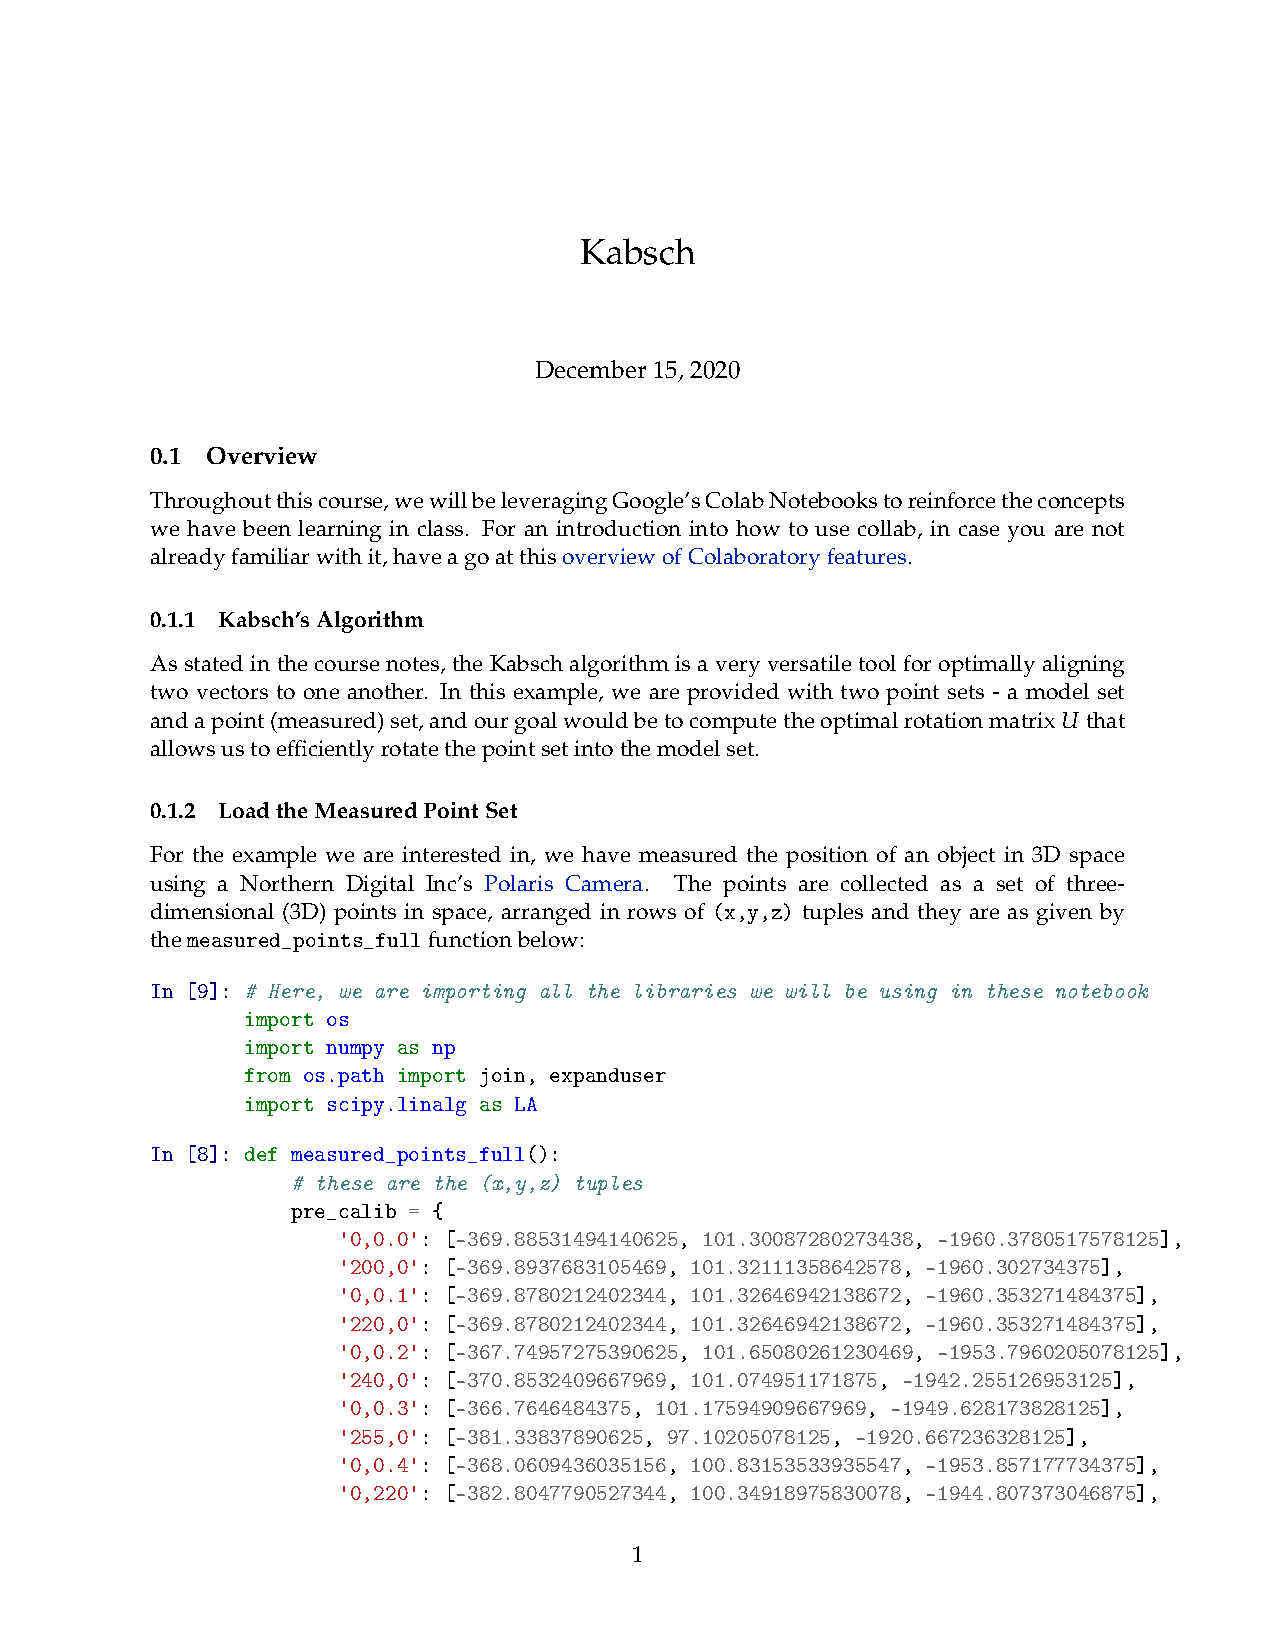
\includepdf[pages=1-]{Kabsch.pdf}

\begin{homework}
	For the following model points $P$ and measured poinyts $Q$, compute the optimal rotation matrices for moving points $Q$ into point $P$. 
	%
	For the three assignments below, report your results within a colab notebook, download the colab notebook as a pdf and upload on Latte.
	\begin{enumerate}
		\item  \begin{align}
			P = \begin{bmatrix}
			-1 & 0 & 0 \\
			%
			0 & 0 & 0 \\
			%
			0 & 1 & 1
			\end{bmatrix},
			%
			\qquad 
			Q = \begin{bmatrix}
			0 & -1 & -1 \\
			0 & -1 & 0 \\
			0 & 0 & 0 \\
			-1 & 0 & 0
			\end{bmatrix}
		\end{align}
		%
		\item \begin{align}
			P = \begin{bmatrix}
			3172.79468418  &  727.52462347  & 7122.70450243 \\
			165.28953155 &  -3552.32467068 & -2045.15346584 \\
			5292.45250241 & -1748.52037006 & -6181.40300009 \\
			1893.07584225  & 5897.19719625  & 3130.41287776
			\end{bmatrix}, 
			\\
			Q = \begin{bmatrix}
			1774.11606309 & -4241.11341178  & 5259.04277742 \\
			6079.70499031  &  -98.14197972 & -3442.0914569 \\
			813.07069876  & 3334.26289147 & -6112.55652513 \\
			1856.72080823 &  2328.86927901  & 6322.16611888 \\
			\end{bmatrix} \nonumber
		\end{align}
		%
		\item For a toy problem, measure the coordinates of an object in the world using your favorite measuring instrument (a 3D camera sensor, iPhone app (e.g. ArkIt), android app e.t.c.). Be sure to record the position of the object at multiple points in world coordinates and make sure that the physical locations of these points are known (these are your model points). Then compute the optimal rotation and translation between the model and measured points.
	\end{enumerate}
\end{homework}

\section{Iterative Closest Point}

\chapter{State Estimation}
\label{chap:state_ext}

The next few topics in this course shall involve the quantification of uncertainty in order to enable a robot navigate, move, or understand its environment via visual or audio sensors. In order to do justice to this topic, we shall soon find out that the concept of putting a value or percentage on how sure we are about a robot's environment shall be very helpful in effective control of our robots. Thus the concept of probability shall greatly aid us in quantifying uncertainty. Even so, we introduce the concept of states, grounded in a mathematical theory that allows the engineer to implement a state through discrete-time systems (since we assume that most implementations shall be done on digital computers). By the \textit{state} of a system, we shall loosely mean ``those variables that provide a complete representation of the internal condition or status of the system at a given time instant." In this sentiment, the states of a motor system may mean currents that flow through the inductive coils, the position and speed of its motor shaft, or the voltage across the coils of a solenoid valve. The states of a military power may include the number of its aircraft carriers, the size and horsepower of its nuclear submarines, the number of enlisted servicemen in its forces e.t.c. For a biological system, the states might include blood sugar levels, heart and respiration rates, or body temperature.

Robot systems may include mobile platforms for extraterrestrial navigation, robotics arms in assembly lines, autonomous cars, or actuated surgical devices that assist surgeons. Our goal is to treat uncertainty. Uncertainty occurs if the robot lacks important information that hinders it from carrying out assigned tasks. We may classify this uncertainty into five different factors, viz.,
%
\begin{enumerate}
	\item \textbf{Environments.} The physical world is inherently unpredictable. While the degree of uncertainty in well-structured environments such as  assembly lines is small, environments such as highways and private homes are highly dynamic and unpredictable.
	%
	\item \textbf{Sensors.} Most sensors have limitations in their perceptual ability arising from noise and the range and the resolution of the sensors. For example, environmental disturbances, weather, lighting conditions limit the information that can be extracted from sensors. Secondly, as to range and resolution, cameras cannot see through walls despite the perceptual range that the spatial resolution of the camera is limited.
	%
	\item \textbf{Models.} In general, models are at best an approximation or a mathematical representation or abstraction of the physical world. As such, model errors are a source of uncertainty that need to be incorporated in modeling robotics problems.
	%
	\item \textbf{Computation.} Being real-time systems, robots require a lot of computation in order to be able to achieve timely-response through sacrificing accuracy.
\end{enumerate}

We will estimate states as they shall represent latent or underlying variables that influence the physical or chemical or financial properties of the system. And in motivating the study of a system's state, we can resolve to many weapons in our estimation arsenal which may include linear state filtering (the simple Kalman filter), nonlinear state filters (the extended Kalman filter, unscented Kalman filter e.t.c.), Bayesian estimation, and \textit{frequentist/classical} estimation approaches. In general, state estimation is an important topic to the engineer because:
%
\begin{itemize}
	\item We may need to implement a feedback controller in order to regulate a system's behavior. If the application was for a surgeon to regulate blood pH levels, we may need to estimate the system's state. Or if the challenge is to adequately position a patient's head to a position in 3D space during cancer stereotactic radiosurgery, we may need to estimate the position and orientation of the patient's head and neck in the inertial frame.
	%
	\item If the states in question are curious enough, we may want to measure these states to understand the faults tolerance of the system in order to perform a good fault identification and prognosis. For example, we might want to estimate the internal states of an aircraft system in flight such that if an aircraft engine fails during flight, we can safely monitor system states in real-time in order to determine how long we can continue flying the aircraft or if we should quickly find a near-by airport where we could land the aircraft for maintenance.
\end{itemize} 
%
In our treatment, therefore, we shall give a brief introduction to linear systems theory, touch upon standard linear filters and then proceed to treat probability theory before we treat nonlinear systems, and decision-making.

\section{Linear Systems}

State-space systems are very important in engineering systems because they allow us 
%
\begin{inparaenum}[(i)]
	\item to gain insight into the characteristics of the system,
	\item be able to predict future behaviors of the system, 
	\item  identify the controllable and observable states of the system.
\end{inparaenum} 
%
The mathematical model of the process allows us to infer the information about the process. State-space models can be classified into linear and nonlinear systems. While most real-world systems are nonlinear, the tools that exist for analyzing and synthesizing nonlinear systems  are well-developed and sophisticated that most nonlinear systems can be approximated by linear systems in order to exercise good control and estimation for real-world applications.

A continuous-time, deterministic linear system can be described by the equations 
%
\begin{align}
	\dot{x} &= Ax + Bu \nonumber \\
	y &= Cx
\end{align}
%
where $x$ is the \textit{state vector} in $\mathbb{R}^n \times 1$, $u$ is the \textit{control vector} in $\mathbb{R}^p \times 1$, and $y$ is an  $\mathbb{R}^n \times 1$ vector. Matrices $A$, $B$, and $C$ are respectively $n\times n$, $n \times p$ and $n \times 1$ in dimension. The matrix $A$ is often called the system matrix, $B$ the input or control matrix, while $C$ is often called the output matrix. $A, B$, and $C$ can be time-varying matrices, in which case the system is linear. Otherwise, the solution to the linear system of equations above is 
%
\begin{align}
	x(t) &= e^{A(t-t_0)} x(t_0) + \int_{t_0}^{t} e^{A(t-\tau)} B u(\tau) d\tau  \\
	y(t) &= C x(t)
	\label{eq:matrix_exp}
\end{align}
%
where $t_0$ is the initial time of the system. If the input control law is zero, then we have a \textit{non-autonomous system} i.e.
%
\begin{align}
	x(t) &= e^{A(t-t_0)} x(t_0) 
\end{align}
%
and because of this, $e^{AT}$ is called the state-transition matrix \ie it describes how the state moves between transitions at different times regardless of external inputs. At $t = t_0$, we have that 
%
\begin{align}
	e^{A \, 0} = I,
\end{align}
%
which is similar to the scalar exponential of a zero. What happens if $x$ is an $n$-element vector? The solution in \eqref{eq:matrix_exp} still remains valid but we must note that the exponential of the matrix becomes interpreted as 
%
\begin{align}
	e^{At} &= \sum_{j=0}^{\infty} \dfrac{(At)^j}{j!} \nonumber \\
	&= \mathcal{L}^{-1} \left[sI - A\right]^{-1} = Q e^{\hat{A}t} Q^{-1}
	\label{eq:matrix_exp_jordan}
\end{align}
%
where the symbol $\mathcal{L}^{-1}$ is the symbol for the inverse Laplace transform and $``s"$ is the Laplace operator. We see that $A$ must be square in order for $e^{At}$ to exist. $Q$ contains the eigenvectors of $A$ and $\hat{A}$ are the Jordan form of $A$.
%
\begin{quiz}
	Write a note about the Jordan form. Also, explain how it can be determined from \eqref{eq:matrix_exp_jordan}.
	% ANS
	% \eqref{eq:matrix_exp_jordan} can be used to define the Jordan form of the matrix. 
\end{quiz}
%
\begin{quiz}
	Does the matrix $A$ commute with its exponential i.e. does $A \, e^{At} = e^{At} \, A$? 
\end{quiz}

The matrix $\hat{A}$ is often diagonal, so that case $e^{\hat{A}t}$ can be computed as
%
\begin{align}
	\hat{A} = \begin{bmatrix}
	\hat{A}_{11} & 0 & \ldots & 0 \\
		0 & \hat{A}_{22} & \ldots 0 \\
		\vdots & \ddots & \ddots & \vdots \\
		0 & \ldots & \ldots & \hat{A}_{nn} 
	\end{bmatrix} \quad 
	%	
	e^{\hat{A}t} = \begin{bmatrix}
	e^{\hat{A}_{11}} & 0 & \ldots & 0 \\
	0 & e^{\hat{A}_{22}} & \ldots 0 \\
	\vdots & \ddots & \ddots & \vdots \\
	0 & \ldots & \ldots & e^{\hat{A}_{nn}}
	\end{bmatrix}
\end{align}

From \eqref{eq:matrix_exp_jordan}, we can write 
%
\begin{align}
	\left[e^{At}\right]^{-1} = e^{-At} = Q e ^{-\hat{A}t} Q^{-1}
\end{align}
%
Since $A$ and $-A$ have eigenvalues that are negative of each other, $e^{At}$ is always invertible.

\begin{example}
	Suppose we are controlling angular heading of a mobile robot (for example, using voltage applied to its wheels' rotor windings in order to generate command velocity along the $x$, $y$, and $z$ heading, i.e. $\theta$, $\omega$ and $\alpha$ respectively). The derivative of the angular velocity vector can be written as 
	%
	\begin{align}
	\dot{\theta} &= \omega + \alpha + 3.5 \omega_1 + 6 \theta_2 \nonumber \\
	\dot{\omega} &= u + 0.1 \theta  + 2.5 \alpha + \omega_1 + \omega_2^2\nonumber \\
		\dot{\alpha} &= \theta_1 + 2 u %\nonumber \\
	\end{align}
	%
	The scalars $\omega_1$, $\omega_2$, $\theta_1$ and $\theta_2$ are acceleration noise terms such as gear backlash, friction, and modeling errors. If our measurement consists of the $\theta$ and $\omega$ states, it follows that we can write the state space equation as 
	%
	\begin{align}
		\begin{bmatrix}
		 \dot{\theta} \\ \dot{\omega} \\ \dot{\alpha}
		\end{bmatrix}
		& =
		\begin{bmatrix}
		0 & 1 & 1 \\
		1 & 0 & 2.5 \\
		0 & 0 & 0
		\end{bmatrix}
		+
		\begin{bmatrix}
		0 \\ 1 \\ 2
		\end{bmatrix} u
		+
		\begin{bmatrix}
		 3.5 \omega_1 + 6 \theta_2 \\
		 \omega_1 + \omega_2^2 \\
		 \theta_1
		\end{bmatrix} \nonumber \\
		%
		y &= \begin{bmatrix}
		1 & 1 & 0
		\end{bmatrix} +
		\begin{bmatrix}
		\theta \\ \omega \\ \alpha
		\end{bmatrix} + \begin{bmatrix}
		{v_x} \\ {v_y} \\ {v_z}
		\end{bmatrix}
	\end{align}
	where $v = [v_x, v_y, v_z]^T$ is the linear velocity vector for  the robot.
\end{example}

\begin{example}
	Suppose that 
	\begin{align}
		A = \begin{bmatrix}
		0 & 1 \\ 0 & 0
		\end{bmatrix}
	\end{align}
	%
	It follows that
	%
	\begin{align}
		e^{At} &= \sum_{j=0}^{\infty} \dfrac{(At)^j}{j!} \nonumber \\
		       &= (At)^0 + (At)^1 + \frac{(At)^2}{2!} +  \frac{(At)^3}{3!} + \ldots \nonumber \\
		       &= I + At
	\end{align}	
	where the last term follows from the fact that $A^k = 0$ for $k>1$ so that 
	%
	\begin{align}
		e^{At} = \begin{bmatrix}
		1 & 0 \\ 0 & 1
		\end{bmatrix}
		+ 
		\begin{bmatrix}
		0 & t \\ 0 & 0
		\end{bmatrix}
		= 
		\begin{bmatrix}
		1 & t \\ 0 & 1
		\end{bmatrix}
	\end{align}
	%
	Using the expression for the inverse Laplace transform earlier, we have 
	%
	\begin{align}
		e^{At} &= \mathcal{L}^{-1}\left[\left(sI-A\right)^{-1}\right] \nonumber \\
		&= \mathcal{L}^{-1}\left(
		\begin{bmatrix}
		s & -1 \\ 0 & s
		\end{bmatrix}^{-1}\right) \nonumber \\
		&= \mathcal{L}^{-1} 
		\begin{bmatrix}
		1/s & 1/s^2 \\ 0 & 1/s
		\end{bmatrix} \nonumber \\
		&= \begin{bmatrix}
		1 & t \\ 0 & 1
		\end{bmatrix}
		\label{eq:example_matrix_eq}
	\end{align}
\end{example}

\begin{homework}
	Find the eigendata of the matrix A in \eqref{eq:example_matrix_eq}. Then determine the following terms using the eigenvector and eigenvalue that you may find:
	$\hat{A}, Q$ and $e^{At}$.
\end{homework}

\begin{homework}
	Produce a one-page report on a control system transfer function.
\end{homework}
%
\section{State Space Standard Forms}
For a linear system, there are many possible state space models that can result in the same \textit{transfer function dynamics}. Therefore, standardizing state space model structures is 
relevant for solving problems in a conformal way. For consider the following input-output system's \textit{linear difference equation\footnote{\begin{quiz}
			What is the difference between a \textit{linear difference equation} and a \textit{linear ordinary differential equation?}
\end{quiz}}}
%
\begin{align}
	y_n + a_1 y_{n-1}  + \ldots + a_{n-1} y_1 + a_n y = b_0 u_n + b_1 u_{n-1} + \ldots + b_{n-1} u_1 + b_n u
\end{align}
%
with $u$ and $y$ serving respectively as the input and output, and $y_n$ serving as the $n$th derivative of $y$ with respect to time. If we take the Laplace transform of both sides, we have
%
\begin{align}
	Y(s) \left(s^n + a_1s^{n-1}+\ldots + a_{n-1}s + a_n\right) = U(s)\left(b_0 s^n + b_1 s^{n-1} + \ldots + b_{n-1} s + b_n\right)
\end{align}
%
so that the transfer function from the input $u$ to the output $y$ can be written as 
%
\begin{align}
	\dfrac{Y(s)}{U(s)} = \dfrac{b_0 s^n + b_1 s^{n-1} + \ldots + b_{n-1} s + b_n}{s^n + a_1s^{n-1}+\ldots + a_{n-1}s + a_n}
	\label{eq:transfer_fcn}
\end{align}

\subsection{Companion form}

In \textit{companion form} representation, the coefficients of the transfer function in \eqref{eq:transfer_fcn} are arranged along its far rows or columns. An example would be 
%
\begin{align}
	\begin{bmatrix} 0 & 0 & 0 & \cdots & 0 & -a_0 \\
	1 & 0 & 0 & \cdots & 0 & -a_1 \\
	0 & 1 & 0 & \cdots & 0 & -a_2 \\
	0 & 0 & 1 & \cdots & 0 & -a_3 \\
	\vdots & \vdots & \vdots &\ddots & \vdots & \vdots \\
	0 & 0 & 0 & \cdots & 1 & -a_{n-1} 
	\end{bmatrix}
\end{align}
%
or
%
\begin{align}
	\begin{bmatrix} -a_{n-1} & -a_{n-2} & -a_{n-3} & \cdots & -a_1 & -a_0 \\
	1 & 0 & 0 & \cdots & 0 & 0 \\
	0 & 1 & 0 & \cdots & 0 & 0 \\
	0 & 0 & 1 & \cdots & 0 & 0 \\
	\vdots & \vdots & \vdots &\ddots & \vdots & \vdots \\
	0 & 0 & 0 & \cdots & 1 & 0 
	\end{bmatrix}
\end{align}

In general, we use the convenient \textit{observable} and \textit{controllable} canonical forms in control theory. They are exactly the transpose of one another and using either for control design simplifies the system structure so that it can be readily manipulated for a desired control.

\subsection{Modal Form}

The modal form is the dual to the companion form. In the modal form, the state matrix is a diagonal matrix with non-repeating eigenvalues such that the control has a unitary influence on each eigenspace, and the output is a linear combination of the contributions from the eigenspaces. That is,
%
\begin{subequations}
	\begin{align}
	A &= \begin{bmatrix} -p_1 & 0 & 0 & \cdots & 0 & 0 \\
	0 & -p_2 & 0 & \cdots & 0 & 0 \\
	0 & 0 & -p_3 & \cdots & 0 & 0 \\
	\vdots & \vdots & \vdots &\ddots & \vdots & \vdots \\
	0 & 0 & 0 & \cdots & 0 & -p_n
	\end{bmatrix} \\
	%
	B &= \begin{bmatrix} 1 \\ 1 \\ \vdots \\ 1 \end{bmatrix} \quad
	%
	C = \begin{bmatrix} c_1 & c_2  & \cdots & c_n \end{bmatrix}
	\end{align}
\end{subequations}
%
\begin{homework}
	Write out the solution to \autoref{eq:companion_ex} in modal form.
\end{homework}

\subsection{Controllable Canonical Form}

When we want to design a controller that leverages the full state of the system (assuming this is known), often the \textit{controllable canonical form} will come in handy. It is expressed as follows:
%
\begin{subequations}
	\begin{align}
	A &= \begin{bmatrix} -a_1 & -a_2 & -a_3 & \cdots & -a_{n-1} & -a_n \\
	1 & 0 & 0 & \cdots & 0 & 0 \\
	0 & 1 & 0 & \cdots & 0 & 0 \\
	0 & 0 & 1 & \cdots & 0 & 0 \\
	\vdots & \vdots & \vdots &\ddots & \vdots & \vdots \\
	0 & 0 & 0 & \cdots & 1 & 0 
	\end{bmatrix} 
	\\
		B &= \begin{bmatrix} 1 \\ 0 \\ \vdots \\ 0 \end{bmatrix}
	\quad
	C = \begin{bmatrix} b_1 & b_2 & b_3 & \cdots & b_n \end{bmatrix}
	\quad 
	D = \begin{bmatrix} b_0 \end{bmatrix}
	\end{align}
\end{subequations}

\begin{example}
	For the system 
	\begin{align}
		\dfrac{Y(s)}{U(s)} = \dfrac{5s^2-s+8}{s^2+4s-2}
	\end{align}
	%
	we can realize the state space representation in canonical form as follows:
	\begin{enumerate}
%		\item First we rewrite the transfer function as 
%		%
%		\begin{align}
%		\dfrac{Y(s)}{U(s)} = \dfrac{s^3 + 5/2s^2-1/2s+4}{s^2+4s-2}
%		\end{align}
		%
		\item Observe that $n$ from \eqref{eq:transfer_fcn} is $3$, \ie the highest $s$ exponent in the given transfer function. 
		%
		\item It follows that we have $a_0= -2$ and $a_1 = 4$; and $b_0 = 5, \, b_1=-1$, \, $b_2 = 8$, so that we can write the state space model as
		%
		\begin{align}
			  \begin{bmatrix}
			  \dot{x}_1 
			  \\
			  \dot{x}_2
			  \end{bmatrix} 
			  &=
			  \begin{bmatrix}
			  0 & 2  \\
			  1 & -4 
			  \end{bmatrix}
			  %			  
			  \begin{bmatrix}
			  {x}_1 
			  \\
			  {x}_2
			  \end{bmatrix} 
			  +
			  %			  
			  \begin{bmatrix}
			  1
			  \\
			  0
			  \end{bmatrix} 			  
			  %			  
			  \begin{bmatrix}
			  {u}_1 
			  &
			  {u}_2
			  \end{bmatrix} \nonumber \\
			  %
			  y &= \begin{bmatrix}
			  -1 & 8
			  \end{bmatrix}
			  %			  
			  \begin{bmatrix}
			  {x}_1 
			  \\
			  {x}_2
			  \end{bmatrix} 
			  + 
			  \bm{u}
		\end{align}
	\end{enumerate}
\end{example}
%
\begin{homework}
	Derive the companion form for the system:
	\begin{align}
	\dfrac{Y(s)}{U(s)} = \dfrac{3s^2-2s+1}{s^2-8s+5}
	\end{align}
	\label{eq:companion_ex}
\end{homework}

The controllable canonical form is helpful in when using the pole placement method for controller design. However, the system's transformation to companion form is based on the controllability matrix which is almost always numerically singular for mid-range orders. It should be avoided for computation when possible.

\subsection{Observable Canonical Form}

In observable canonical form, the transfer function coefficients of \eqref{eq:transfer_fcn} are written in the rightmost column of the $A$ matrix similar to the companion canonical form but the $B$ matrix takes a different form. It is given as follows:
%
\begin{align}
A &= \begin{bmatrix} 0 & 0 & 0 & \cdots & 0 & -a_0 \\
1 & 0 & 0 & \cdots & 0 & -a_1 \\
0 & 1 & 0 & \cdots & 0 & -a_2 \\
0 & 0 & 1 & \cdots & 0 & -a_3 \\
\vdots & \vdots & \vdots &\ddots & \vdots & \vdots \\
0 & 0 & 0 & \cdots & 1 & -a_{n-1} 
\end{bmatrix} \\
%
B &= \begin{bmatrix}
	b_n - a_n b_0 \\
	%	
	b_{n-1} - a_{n-1} b_0 \\
	%	
	b_{n-2} - a_{n-2} b_0 \\
	%	
	\vdots \\
	%
	b_{1} - a_{1} b_0 \\
\end{bmatrix}
%
\quad 
C = \begin{bmatrix}
 0  & 0 & \ldots & 1
\end{bmatrix}, \quad D = b_0
 \end{align}
%
This observable canonical form is ill-conditioned for most state-space computation. It should be avoided for computation when possible as its controllability matrix is almost always numerically singular for mid-range orders.

The observable and controllable canonical forms' matrices are respectively transposes of one another.

%
\begin{homework}
Transform the exercise of \ref{eq:companion_ex} to observable canonical form.
\end{homework}

\section{Nonlinear Systems}

\textit{All the world is a nonlinear system. He linearized to the right. He linearized to the left. Till nothing was right. And nothing was left. -- Stephen Billings.}

Our treatment of dynamical so far has involved linear systems. These are optimistic models of the real world as in the reality, nothing is really linear. In general, a nonlinear system is a system which is not linear \ie, does not satisfy the \textit{principle of superposition}. Even a simple resistor exhibits nonlinearity. However, we utilize Ohm's law in approximating the dynamics of a resistor. This is because the equation is valid over a wide enough operating range. In this light, while we may say linear systems do not exist in real life, linear systems are a useful tool for describing nonlinear systems. We will write a general nonlinear system with the equation
%
\begin{align}
	\dot{x} &= f(x, u, w) \nonumber \\
	y &= h(x, v)
	\label{eq:nlnr}
\end{align}
%
where $f(\cdot)$ and $h(\cdot)$ are arbitrary vector valued functions, $w$ denotes the process noise, and $v$ denotes the measurement noise. We have a \textit{time-varying} system if $f(\cdot)$ and $h(\cdot)$ are explicit functions of $t$, otherwise, the system is termed \textit{time-invariant}. Suppose that %
\begin{align}
	f(x, u, w) &= Ax + Bu + w; \text{  and  } \\
	 h(x,v) &= Hx + v,
\end{align}
%
then the system is linear. Otherwise, the system is nonlinear.

Often, we will need to linearize a nonlinear system in order to properly analyze its stability properties or synthesize its parameters for a particular control application. Suppose we have a nonlinear vector function $f(\cdot)$ of a scalar $x$, we can expand $f(x)$ in a Taylor series around some nominal operating point, $x = \bar{x}$ i.e.
%
\begin{align}
	f(x) = f(\bar{x}) + \dfrac{\partial f}{\partial x} \bigg\rvert_{\bar{x}} \tilde{x}+ \dfrac{1}{2!} \dfrac{\partial^2f}{\partial x^2} \bigg\rvert_{\bar{x}} \tilde{x}^2 + \dfrac{1}{3!} \dfrac{\partial^3f}{\partial x^3} \bigg\rvert_{\bar{x}} \tilde{x}^3 +  \ldots
\end{align}
%
where $\tilde{x} = x - \bar{x}$. For a $2 \times 1$ vector $x$, we can write $f(x)$ as follows:
%
\begin{align}
	f(x) &= f(\bar{x}) + \dfrac{\partial f}{\partial x_1} \bigg\rvert_{\bar{x}} \tilde{x}_1 + \dfrac{\partial f}{\partial x_2} \bigg\rvert_{\bar{x}} \tilde{x}_2 + \dfrac{1}{2!} \left(\dfrac{\partial^2f}{\partial x_1^2} \bigg\rvert_{\bar{x}} \tilde{x}_1^2 + \dfrac{\partial^2f}{\partial x_2^2} \bigg\rvert_{\bar{x}} \tilde{x}_2^2 + 2 \dfrac{\partial ^2 f}{\partial x_1 x_2}\bigg \rvert_{\bar{x}} \tilde{x}_1 \tilde{x}_2 \right) + \nonumber \\
	%
	& 
	%
	\dfrac{1}{3!} \left(\dfrac{\partial^3f}{\partial x_1^3} \bigg\rvert_{\bar{x}} \tilde{x}_1^3 + \dfrac{\partial^3f}{\partial x_2^3} \bigg\rvert_{\bar{x}} \tilde{x}_2^3 + 3 \dfrac{\partial ^3 f}{\partial x_1^2 x_2}\bigg \rvert_{\bar{x}} \tilde{x}_1^2  \tilde{x}_2 + 3 \dfrac{\partial ^3 f}{\partial x_1 x_2^2}\bigg \rvert_{\bar{x}} \tilde{x}_1  \tilde{x}_2^2  \right) + \ldots
\end{align}
 %
 which can be compactly written as 
 %
 \begin{align}
 	f(x) & = f(\tilde{x}) + \left(\tilde{x}_1 \dfrac{\partial}{\partial x_1} + \tilde{x}_2 \dfrac{\partial}{\partial x_2}\right)f\bigg\rvert_{\bar{x}} +
 	%
 	\dfrac{1}{2!} \left(\tilde{x}_1 \dfrac{\partial}{\partial x_1} + \tilde{x}_2 \dfrac{\partial}{\partial x_2}\right)^2f\bigg\rvert_{\bar{x}} + \nonumber \\
 	%
 	& 
 	%
 	\qquad \dfrac{1}{3!}\left(\tilde{x}_1 \dfrac{\partial}{\partial x_1} + \tilde{x}_2 \dfrac{\partial}{\partial x_2}\right)^3f\bigg\rvert_{\bar{x}} + \ldots
 \end{align}
%
And when $n$ is an $n\times 1$ vector, the vector $f(x)$, expanded in a Taylor series becomes
%
\begin{align}
	f(x) &=  f(\tilde{x}) + \left(\tilde{x}_1 \dfrac{\partial}{\partial x_1} + \ldots + \tilde{x}_n \dfrac{\partial}{\partial x_n}\right)f\bigg\rvert_{\bar{x}} +
	%
	\dfrac{1}{2!} \left(\tilde{x}_1 \dfrac{\partial}{\partial x_1} + \ldots + \tilde{x}_n \dfrac{\partial}{\partial x_n}\right)^2f\bigg\rvert_{\bar{x}} + \nonumber \\
	%
	& 
	%
	\qquad \dfrac{1}{3!}\left(\tilde{x}_1 \dfrac{\partial}{\partial x_1} + \ldots + \tilde{x}_n \dfrac{\partial}{\partial x_n}\right)^3f\bigg\rvert_{\bar{x}} + \ldots
\end{align}
%
Suppose we define the operation $D^k_{\tilde{x}}f$ as 
%
\begin{align}
	D^k_{\tilde{x}} = \left(\sum_{i=1}^{n} \tilde{x}_i \dfrac{\partial}{\partial x_i}\right)^k f(x) \bigg \rvert_{\bar{x}}
\end{align}
%
so that we can define $f(x)$ in Taylor series form as 
%
\begin{align}
	f(x) &= f(\bar{x}) + D_{\tilde{x}} f + \dfrac{1}{2!} D^2_{\tilde{x}} f + \dfrac{1}{3!} D^3_{\tilde{x}} f + \ldots \\
	& = f(\bar{x}) + D_{\tilde{x}} f +o(\delta).
\end{align}
%
If $f(x)$ is ``sufficiently smooth", it is not far fetched to see that the above equation turns to
%
\begin{align}
	f(x) \approx f(\bar{x}) + D_{\tilde{x}} f \approx  f(\bar{x}) + \dfrac{\partial f}{\partial x}\rvert_{\bar{x}} \tilde{x} \approx  f(\bar{x}) + A \tilde{x}.
\end{align} 
%
since $o(\delta)$ implies that higher order terms satisfy $\lim_{\delta\rightarrow 0} \frac{o(\delta)}{\delta}=0$, and $A = \dfrac{\partial f}{\partial x}\bigg\rvert_{\bar{x}}$.

Recall \eqref{eq:nlnr}, if we choose a nominal operating point $(\bar{x}, \bar{u}, \bar{w})$ and carry out a Taylor series expansion about this nominal point of the nonlinear system of equations, for the state part, we have

\begin{align}
	\dot{x} &= f(x, u, w) \nonumber \\
	&\approx f(\bar{x}, \bar{u}, \bar{w}) + \dfrac{\partial f}{\partial x}\bigg\rvert_{(\bar{x}, \bar{u}, \bar{w})} (x - \bar{x}) +  \dfrac{\partial f}{\partial u}\bigg\rvert_{(\bar{x}, \bar{u}, \bar{w})} (u - \bar{u}) +  \dfrac{\partial f}{\partial w}\bigg\rvert_{(\bar{x}, \bar{u}, \bar{w})} (w - \bar{w}) + o(\delta)  \\
	%
	& = 	 f(\bar{x}, \bar{u}, \bar{w}) + \dfrac{\partial f}{\partial x}\bigg\rvert_{(\bar{x}, \bar{u}, \bar{w})} \tilde{x} +  \dfrac{\partial f}{\partial u}\bigg\rvert_{(\bar{x}, \bar{u}, \bar{w})} \tilde{u} +  \dfrac{\partial f}{\partial w}\bigg\rvert_{(\bar{x}, \bar{u}, \bar{w})} \tilde{w} + o(\delta) \nonumber \\
	%
	& = 	 \dot{\bar{x}} + A \tilde{x} +  B \tilde{u} +  L \tilde{w} \nonumber 
\end{align}
%
Since $\tilde{w}$ is a noise term, it suffices that $\tilde{w} = \bar{w}= w$ so that we can write
%
\begin{align}
	\dot{x} - \dot{\bar{x}} &=  A \tilde{x} +  B \tilde{u} +  L w \qquad \text{ or }\nonumber \\
	\dot{\tilde{x}} &= A \tilde{x} +  B \tilde{u} +  L w.
	\label{eq:nlnr_dev}
\end{align}
%
In other words, we have a linear equation for the deviations of the nonlinear system from the nominal system. It is therefore reason that as long as the deviations are minute enough, the linearization will be valid and the linear equation of \eqref{eq:nlnr_dev} will describe the nonlinear system \eqref{eq:nlnr} well enough. 

In a similar vein, the measurement equation from \eqref{eq:nlnr} will be approximated with the Taylor series expansion about the nominal operating point $(\bar{x}, \bar{u})$ as follows:
%
\begin{align}
	y &= h(x, u) \nonumber \\
	  & \approx h(\bar{x}, \bar{u}) + \dfrac{\partial h}{\partial x}\bigg\rvert_{(\bar{x}, \bar{\nu})} \tilde{x} +  \dfrac{\partial h}{\partial \nu}\bigg\rvert_{(\bar{x}, \bar{\nu})} \tilde{\nu} + o(\delta)  \\
	  &= \bar{y} + C \tilde{x} + D \tilde{\nu} \qquad  \text{ or } \nonumber \\
	  \tilde{y} &= C  \tilde{x} + D \tilde{\nu}.
\end{align}
%
It follows that we can ``solve" a nonlinear control problem by finding linear operating regions whereby we can solve the control problem, after which we can obtain locally linear solutions for the nonlinear control problem.

\begin{example}
	Consider the longitudinal flight control of a hypersonic aircraft cruising at a Mach number of $15$ at an altitude of $110,000ft$. The dynamic equations are \cite{StengelHypersonic}
	%
	\begin{subequations}
		\begin{align}
			\dot{V} &= \left(T \cos \alpha - D\right)/m - \mu \sin \gamma / r^2  \\
			\dot{\gamma} &= \left(L + T \sin \alpha\right)/mV - \left[(\mu - V^2 r) \cos \gamma\right]/(Vr^2) \\
			\dot{h} &= V \sin \gamma \\
			\dot{\alpha} &= q - \dot{\gamma} \\
			\dot{q} &= M_{yy} / I_{yy}
		\end{align}
	\label{eq:hypersonic_dyn}
	\end{subequations}
where
%
\begin{subequations}
	\begin{align}
		L &= \frac{1}{2} \rho V^2 S C_L \\
		D &= \frac{1}{2} \rho V^2 S C_D \\
		T &= \frac{1}{2} \rho V^2 S C_T.
	\end{align}
\end{subequations}
%
Here, $\alpha$ is the angle of attack, $\gamma$ is the flight path angle, $rad$, $r$ is the radial distance from the center of the Earth, $20,903,500$ft, $C_T$ is the thrust coefficient, $C_D$ is the drag coefficient, $C_L$ is the lift coefficient, $L$ is the lift, $D$ is the drag in $lbf$, $h$ is the altitude, $T$ is the thrust in $lbf$, $V$ is the velocity in $ft/sec$, $m$ is the mass, $9375$ slugs, $q$ is the pitch rate in $rad/sec$, $S$ is the reference area, $3603 ft^2$, $I_{yy}$ is the moment of inertia, $7 \times 10^6$ slug-ft$^2$, $M_{yy}$ is the pitching moment in lbf-ft, $\mu$ is the gravitational constant, $1.39 \times 10^16 ft^3/s^2$.

We can write the state space vector of the dynamics as follows:
\[
	\dot{x} = \begin{bmatrix}
				\dot{x}_1 & \dot{x}_2 & \dot{x}_3 & \dot{x}_4 & \dot{x}_5
	\end{bmatrix} = \begin{bmatrix}
	\dot{V} & \dot{\gamma} & \dot{h} & \dot{\alpha} & \dot{q}
\end{bmatrix}
\].

So that the \textit{nonlinear} dynamics of the hypersonic aircraft at the specified cruising altitude of $110,000$ ft and Mach number 15 becomes
%
\begin{subequations}
	\begin{align}
		\dot{x}_1 & = \frac{1}{2m}\rho S \left(C_T \cos x_4 - C_D\right) x_1^2 - \frac{\mu}{r^2} \sin x_2 \\
		\dot{x}_2 &=  \left(\frac{1}{2m}\rho S C_L - \frac{\mu}{x_1^2r^2}\right) x_1 + \frac{x_1}{r} \cos x_2 +\frac{1}{2m}\rho S C_D \sin x_4 \\
		\dot{x}_3 &= x_1 \sin x_2 \\
		\dot{x}_4 &= - \left(\frac{1}{2m}\rho S  C_L - \frac{\mu}{x_1^2r^2}\right) x_1 - \frac{x_1}{r} \cos x_2 -\frac{1}{2m}\rho S C_D \sin x_4 + x_5   \\
		\dot{x}_5 &= M_{yy}/I_{yy}
	\end{align}
\end{subequations}
%
Following our earlier argument, we proceed to linearize the dynamics by first finding the Jacobian with respect to the  state transition matrix, $x$:
%
\begin{align}
	A &= \dfrac{\partial f}{\partial x} \nonumber \\%\bigg\rve \\
	  &= \begin{bmatrix}
	  	\frac{1}{m}\rho S \left(C_T \cos x_4 - C_D\right) x_1 & - \frac{\mu}{r^2}\cos x_2 & 0 & -\frac{1}{2m}\rho S C_T \sin x_4 x_1^2 & 0 \\
	  	\frac{1}{2m}\rho S C_L - \frac{\mu}{r^2 \, x_1^2} +  \frac{1}{r} \cos x_2 &  -\frac{x_1}{r} \sin x_2 & 0 & \frac{1}{2m}\rho S C_D \cos x_4 & 0 \\
	  	\sin x_2 & x_1 \cos x_2 & 0 & 0 & 0 \\
	  	%
	  	- \frac{1}{2m}\rho S C_L - \frac{1}{r} \cos x_2 - \frac{\mu}{r^2 x^2_1} & \frac{x_1}{r} \sin x_2 & 0 & -\frac{1}{2m}\rho S C_D \cos x_4 & 1 \\
	  	0 & 0 & 0 & 0 & 0
	  \end{bmatrix}.
\end{align}

Similarly, the input matrix can be obtained by finding the Jacobian with respect to the lift, $L$, drag $D$, and thrust, $T$,  are
%
\begin{align}
	B &= \dfrac{\partial f}{\partial u} \\
	  &= \begin{bmatrix}
		  	0 & -1/m & 0 \\
		  	1/mV & 0 & \frac{\sin \alpha}{mV} \\
		  	0 & 0 & 0 \\
		  	0 & 0 & 0 \\
		  	0 & 0 & 0
	  \end{bmatrix}
\end{align}
%
so that the linear system 
\begin{align}
	\dot{\tilde{x}} = A \tilde{x} + B \tilde{u} 
\end{align}
%
approximately describes the nonlinear hypersonic aircraft's deviation from its nominal value $\bar{x}$. We can simulate the lift, drag and thrust with the following nominal control values: $L = \sin 2 \pi t$, $D= \cos 2\pi t$, $T = 2L - D$ to find the nominal state trajectory $\bar{x}$.
\end{example}

%\chapter{Manipulator Kinematics}  
\label{chap:manip}

 
Recommended Text Readings: 
\begin{itemize}
 \item \cite[Chapter 3]{MurrayBook}
 %
 \item \cite{Brockett1990}
 %
 \item \cite[Chapter 4]{LynchBook}
\end{itemize}

At issue in this chapter is characterizing the \textit{motion} of a robot based on the position and orientation of the links of the robot (in the case of rigid bodies). We will leave discussion of the forward or differential kinematics of soft robots to a future discussion but we will briefly discuss it in class. First off, based on the first chapter of ~\cite{Hunt1983}'s Kinematic Geometry of Mechanisms, we recollect that there are six primitive types of joints constructed from the so-called \textit{lower pairs} of mechanisms, which all exercise a subgroup of \textit{SE(3)} when they are actuated.


\section{Forward kinematics}
%
Formally, we define the \textit{forward kinematics of a robot as a means of finding the configuration of the end-effector when we are given only the relative configurations of each pair of adjacent links of the robot}. For an open-loop kinematic chain, these adjacent links are the joint angles while for a parallel robot, they are the link lengths of the robot's legs. A similar definition applies to a semi-rigid multi-dof soft robot, whereupon we are tasked with finding the orientation of the tool frame given a characterization of the \textit{deformation} of the adjoining soft or semi-rigid links of the soft robot's body. 
%
\begin{figure}[tb!]
	\centering
	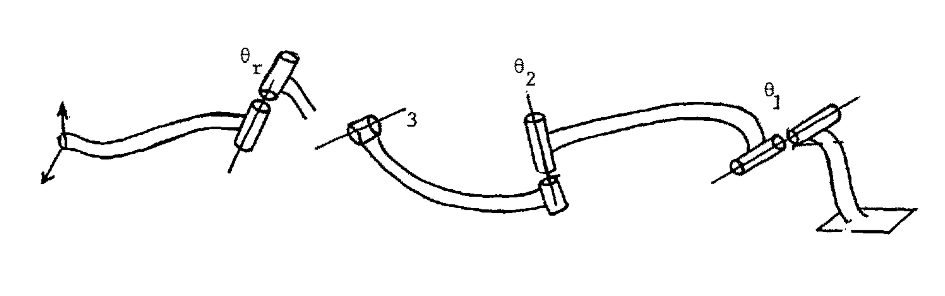
\includegraphics[width=.8\columnwidth]{figures/manip.png}
	\caption{An open kinematic chain. Reprinted from \cite{Brockett1990}.}
	\label{fig:manip}
\end{figure}
%
\begin{figure}[tb!]
	\centering
	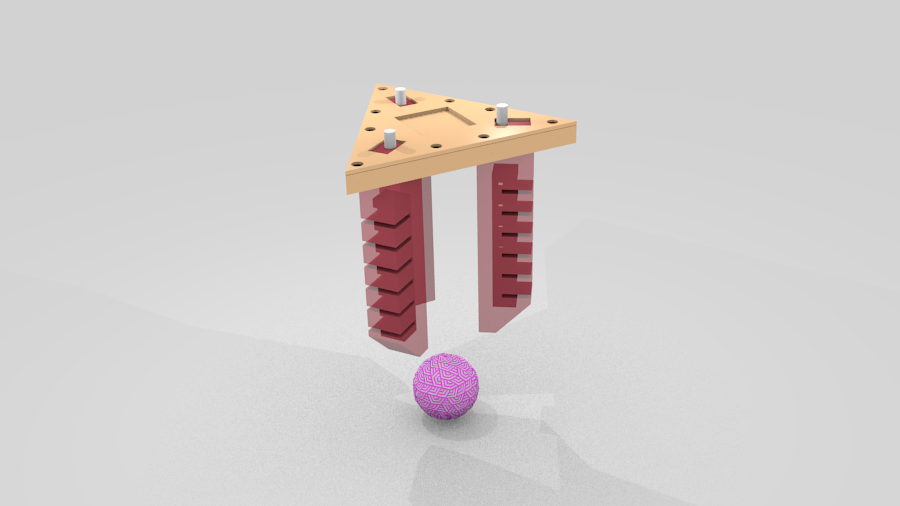
\includegraphics[width=.8\columnwidth]{figures/pneunets.png}
	\caption{The Pneunets Soft Robot}
	\label{fig:pneunets}
\end{figure}
%

\subsection{Screw Axes and  Base Frame}

For consider the kinematic chain of \autoref{fig:manip}. Suppose that we fix a right-handed triad of orthogonal vectors at the tip of each member of the chain, the\textit{ joint space} $Q$ of the robot is the set of all possible values of the joint variables of the robot, which happens to also be the C-space of the robot given that the joint angles completely determine the locations of every link in the robot. 
Similarly, for the soft robot of \autoref{fig:pneunets}, we construct the forward kinematics in a similar fashion; only this time, we do not parameterize the robot links with the joint angles but with the appropriate representation of the deformation of the each pneunet link: an example of a common parameterization approach is to use differential kinematics for arc on the soft robot's body~\cite{Hannan2003}.
%%

For the arm of \autoref{fig:manip}, we may consider that every joint applies a screw motion to all links that protrude from the robot. We take each joint to be displaced by some angle $\theta_i$ so that the end-effector undergoes a displacement of the form $e^{\hat{\xi}_i \theta_i}\homo_i$. The cumulative effect of the robot links on the end-effector is given as (following the notation of \autoref{fig:lienotations}),
%
\begin{align}
\homo_{st}(\theta_1, \ldots, \theta_l) = e^{\hat{\xi}_1 \theta_1}\,e^{\hat{\xi}_2 \theta_2}  \, \ldots e^{\hat{\xi}_l \theta_l} \homo_{st}(0)
\label{eq:fwd_kine}
\end{align}
%
\textit{where $S$ denotes the spatial frame, typically located at the base or shoulder of the robot and $T$ denotes the tool frame, typically situated at the robot's end-effector}. For the system of \eqref{eq:fwd_kine}, we say $\xi_i$ is the twist coordinate of the $i'th$ joint. The equation is the result of moving $\theta_{i+1}$ first before $\theta_i$ while keeping $\theta_i$ fixed. On the other hand, if we reverse the order of the rotations, that would correspond to moving the $i'th$ axis and then rotating the $(i+1)'th$ axis about the new axis, \ie,
%
\begin{align}
	\xi_{i+1}^\prime = \text{Ad}_{e^{\hat{\xi}_i \theta_i}} \xi_{i+1}.
\end{align}
%
We note that the the twist for a revolute joint takes the following form
%
\begin{align}
	\xi_i = \left(\begin{array}{c}
	-\omega \times q_i \\ q_i
	\end{array}\right)
\end{align}
%
where $\omega_i \in \bb{R}3$, is the unit vector in the direction of the twist axis and $q_i \in \bb{R}^3$ is a point along that axis. For a prismatic joint, we have $\xi_i = (v_i, 0)^T$ where $v_i$ is a unit vector along the direction of translation.

\begin{figure}
	\centering
	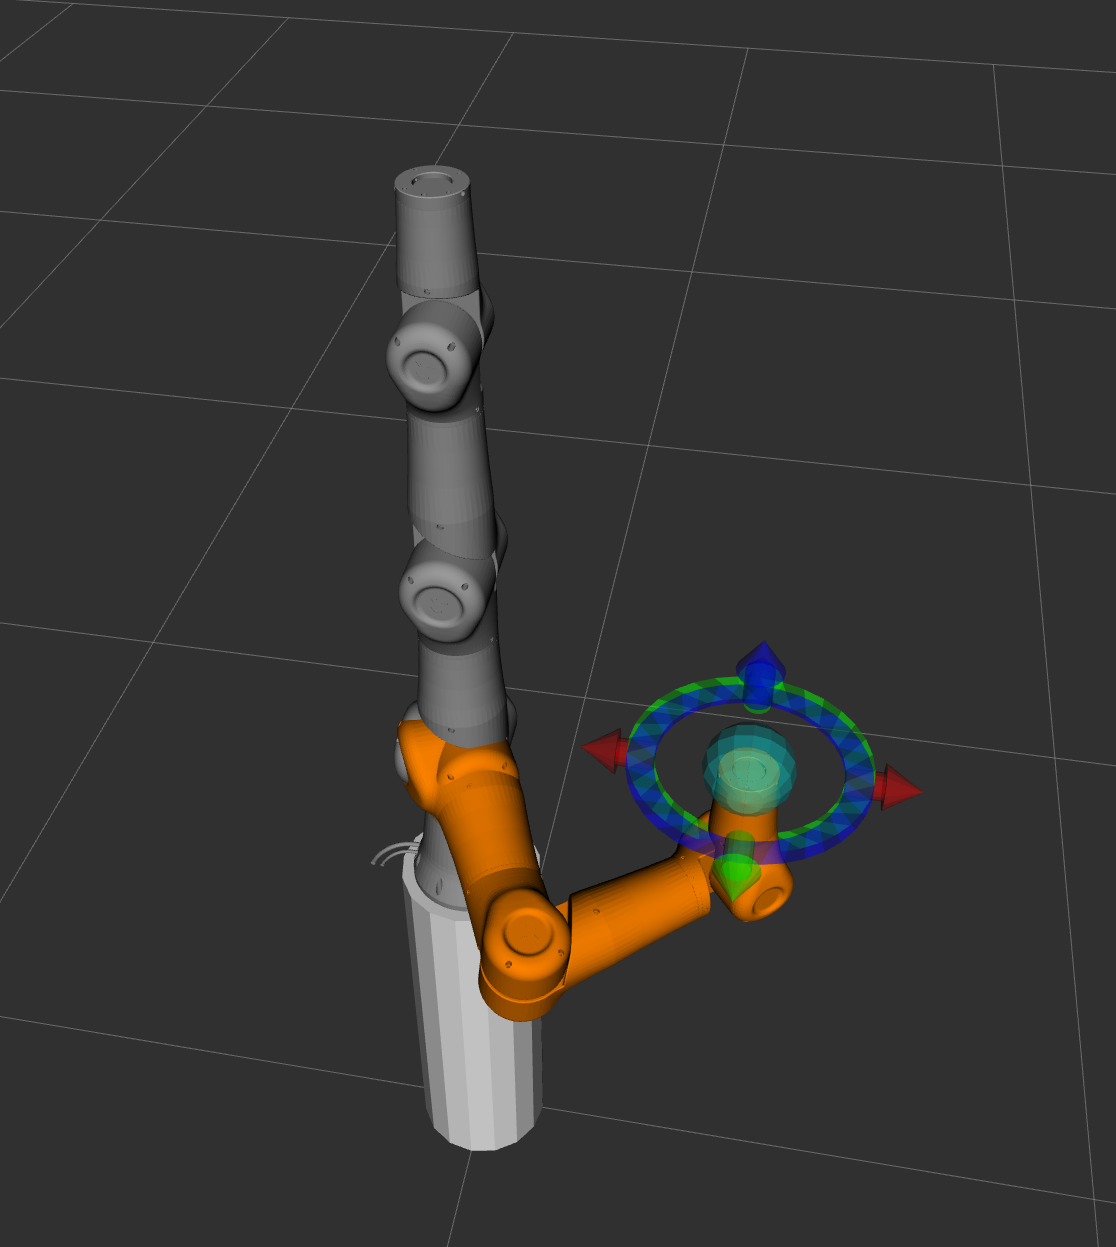
\includegraphics[width=\columnwidth]{figures/torobo7.png}
	\caption{Forward Kinematic Planning for The Torobo 7 Arm}
	\label{fig:torobo7}
\end{figure}
%
\begin{example}
	Consider the Tokyo Robotics (Torobo) arm of \autoref{fig:torobo7}, which is made up of seven joints (six actually, but for now we will assume there is a planar wrist at the end-effector for grasping). The Cartesian coordinates triad are as shown in the orange-colored configuration wherin the blue axis is z, the red axis is $y$-axis and the green axis denotes the $x$-axis. We will take the home position of the robot to be when all joint angles have their angles as $\theta_i = 0$ (this corresponds to the gray pose in the figure). The target pose of the arm is the orange-linked arm shown. The forward kinematics problem would be that given all the six joint angles, and link lengths, find the end-effector pose. We will be leveraging Brockett's product of exponential formula in solving this problem.
	
	For now, suppose the spatial frame is at the base of the robot and the tool frame is on the end-effector. We will for the moment assume that the end-effector is posed at an angle $\theta_7= 0$ as well in the reference frame (colored in gray). The transformation from the base frame to the tool frame is at $\theta = 0$ so that we have from \eqref{eq:fwd_kine}
	%
	\begin{subequations}
		\begin{align}
		&g_{st}(\theta_1,\theta_2,\theta_3,\theta_4,\theta_4, \theta_5, \theta_6, \theta_7) =	e^{\hat{\xi}_1 0}\,e^{\hat{\xi}_2 0},  \, \ldots, e^{\hat{\xi}_l 0} \homo_{st}(0)   \\
		%
		g_{st}(\bm{\theta}) & = g_{st}(0) = \left(\begin{array}{cc}
		\rot(\theta=0) & d \\
		0 & 1
		\end{array} 
		\right) = \left(
		\begin{array}{cc}
		\identity & \left(\begin{array}{c}
		0 
		\\
		%
		0
		\\
		%
		\sum_{i=1}^{i=6} l_i
		\end{array}\right)  \\
		0 & 1
		\end{array} \right).
		\end{align}
	\end{subequations}
\label{ex:torobo7}
\end{example}

\subsection{Screw Axes in Tool Frame}
%
Now, consider again \eqref{eq:fwd_kine}, and recall the properties of the exponential map as given in Def. \autoref{def:exp_map}, we can write 
%
\begin{subequations}
	\begin{align}
	e^{\homo^{-1}P\homo} &= \homo^{-1} e^{P} \homo \\
	\homo \, e^{\homo^{-1}P\homo} &= \homo \, \homo^{-1} e^{P} \homo = e^{P} \homo 
	\end{align}
	\label{eq:mat_exp_reorder}
\end{subequations}
%
Reordering \eqref{eq:fwd_kine} by repeatedly applying \eqref{eq:mat_exp_reorder}, we find that
%
\begin{subequations}
	\begin{align}
	\homo_{st}(\theta_1, \ldots, \theta_l) &= e^{\hat{\xi}_1 \theta_1}\,e^{\hat{\xi}_2 \theta_2}  \, \ldots e^{\hat{\xi}_l \theta_l} \homo_{st}(0) \\
	%
	&= e^{\hat{\xi}_1 \theta_1}\,e^{\hat{\xi}_2 \theta_2}  \, \ldots \homo e^{\homo^{-1} \twistmap_l \homo \theta_l}  \\
	%
	&= e^{\hat{\xi}_1 \theta_1}\,e^{\hat{\xi}_2 \theta_2}  \, \ldots \homo e^{\homo^{-1} \twistmap_{l-1}\homo\theta_{l-1}} e^{\homo^{-1} \twistmap_{l} \homo \theta_l}  \\
	%
	&= e^{\hat{\xi}_1 \theta_1}\,\homo e^{\homo^{-1} \twistmap_{2}\homo\theta_{2}}   \, \ldots e^{\homo^{-1} \twistmap_{l-1}\homo\theta_{l-1}} e^{\homo^{-1} \twistmap_{l} \homo \theta_l}   \\
	%
	&= \homo e^{\homo^{-1} \twistmap_{1}\homo\theta_{1}}  \, e^{\homo^{-1} \twistmap_{2}\homo\theta_{2}}   \, \ldots e^{\homo^{-1} \twistmap_{l-1}\homo\theta_{l-1}} e^{\homo^{-1} \twistmap_{l} \homo \theta_l}  
	\end{align}
	\label{eq:fwd_kine_rev}	
\end{subequations}
%
or 
%
\begin{tcolorbox}[title=Exponential Map in Tool Frame]
	\begin{align}
		\homo_{st}(\theta_1, \ldots, \theta_l) &= \homo e^{\hat{\bodyform}_1\theta_{1}}  \, e^{\hat{\bodyform}_2 \theta_{2}}   \, \ldots e^{\hat{\bodyform}_{l-1} \theta_{l-1}} e^{\hat{\bodyform}_{l} \theta_l} 
	\end{align}
	where $\hat{\bodyform}_i = \homo^{-i} \twistmap_{i}\homo^{i}$ is referred to as the \textbf{body form} of the POE formula. The expression in \eqref{eq:fwd_kine} is notably called the \textbf{space form} of the POE formula.
\end{tcolorbox}

\section{Manipulator parameterization with twists}
%
In the example of \autoref{ex:torobo7}, we can construct the twists for the revolute joints as 
%
\begin{align}
	\omega_1 = \omega_2 = \ldots = \omega_7 = \left(\begin{array}{c}
	0 \\ 0 \\ 1
	\end{array}\right)
\end{align}
%
so that we can choose axis points 
%
\begin{align}
	q_1 &= \left(\begin{array}{c}
	0 \\ 0 \\ l_0
	\end{array}\right) \, 
	%
	q_2 = \left(\begin{array}{c}
	0 \\ 0 \\ l_1
	\end{array}\right) \, 
	%
	q_3 = \left(\begin{array}{c}
	0 \\ 0 \\ l_1 + l_2
	\end{array}\right) \, 
	%
	q_4 = \left(\begin{array}{c}
	0 \\ 0 \\ l_1 + l_2 + l_3
	\end{array}\right) \, 
	%
%	q_4 = \left(\begin{array}{c}
%	0 \\ 0 \\ \sum_{i=1}^{i=4} l_i
%	\end{array}\right) 
	\\
	%	
	q_5 &= \left(\begin{array}{c}
	0 \\ 0 \\  \sum_{i=1}^{i=4} l_i
	\end{array}\right) \, 
	%
	q_6 = \left(\begin{array}{c}
	0 \\ 0 \\  \sum_{i=1}^{i=5} l_i
	\end{array}\right) \, 
	%
	q_7 = \left(\begin{array}{c}
	0 \\ 0 \\  \sum_{i=1}^{i=6} l_i
	\end{array}\right).
\end{align}
%
It follows that we may write the twist as 
%
\begin{subequations}
	\begin{align}
	\xi_1 &= \left(\begin{array}{c}
	0 \\ 0 \\ 0 \\ 0\\ 0 \\ 0 
	\end{array}\right) \, 
	%
	\xi_2 = \left(\begin{array}{c}
	0 \\ 0 \\ 0 \\ 0\\ 0 \\ l_1
	\end{array}\right) \, 
	%
	\xi_3 = \left(\begin{array}{c}
	0 \\ 0 \\ 0 \\ 0 \\ 0 \\ l_1 + l_2
	\end{array}\right) \, 
	%
	\xi_4 = \left(\begin{array}{c}
	0 \\ 0 \\0 \\ 0 \\  l_1 + l_2 + l_3
	\end{array}\right) \, \\
	%\end{align}
	%%
	%\begin{align}
	\xi_5 &= \left(\begin{array}{c}
	0 \\ 0 \\ 0 \\ 0 \\ 0 \\ \sum_{i=1}^{i=4} l_i
	\end{array}\right) \, 
	%
	\xi_6 = \left(\begin{array}{c}
	0 \\ 0 \\  0 \\ 0 \\ 0 \\ \sum_{i=1}^{i=5} l_i
	\end{array}\right) \, 
	%
	\xi_7 = \left(\begin{array}{c}
	0 \\ 0 \\   0 \\ 0 \\ 0 \\ \sum_{i=1}^{i=6} l_i
	\end{array}\right)
	\end{align}
\end{subequations}
%
where the screw axes in the base frame are as given in \autoref{tab:torobo_screw_space_form}
%
\begin{table}[tbph!]
	\caption{Table of Screw Axes for the Torobo Arm.}
	\centering
	\begin{tabular}{|c|c|c|| c|c|c|}
		\hline \rule[-2ex]{0pt}{5.5ex}  
		$i$ & $\omega_i$ & $v_i$ & $i$ & $\omega_i$ & $v_i$\\
		\hline \rule[-2ex]{0pt}{5.5ex}  
		1  & (0, 0, 0) & (0, 0, 0) & 4  & (0, 0, $l_1+l_2+l_3$) & (0, 0, 0) \\	
		\hline \rule[-2ex]{0pt}{5.5ex}  
		2  & (0, 0, $l_1$) & (0, 0, 0) & 5  & (0, 0, $l_1+l_2+l_3+l_4$) & (0, 0, 0)  \\
		\hline \rule[-2ex]{0pt}{5.5ex}  
		3  & (0, 0, $l_1+l_2$) & (0, 0, 0) & 6  & (0, 0, $l_1+l_2+l_3+l_4+l_5$) & (0, 0, 0)  \\
		\hline \rule[-2ex]{0pt}{5.5ex}  
		7  & (0, 0, $l_1+l_2+l_3+l_4+l_5+l_6$) & (0, 0, 0)  & 7  & (0, 0, $l_1+l_2+l_3+l_4+l_5+l_6$) & (0, 0, 0) \\
		\hline
	\end{tabular}
\label{tab:torobo_screw_space_form}
\end{table}
%
We may now write the various exponents as 
%
\begin{subequations}
	\begin{align} 
	e^{\hat{\xi}_1 \theta_1} &= \left(\begin{array}{cccc}
	\cos \theta_1 & -\sin \theta_1 & 0 & 0 \\
	\sin \theta_1 & \cos \theta_1 & 0 & 0 \\
	0 & 0 & 1 & 0 \\
	0 & 0 & 0 & 1
	\end{array}\right), \quad
	%	
	e^{\hat{\xi}_2 \theta_2} = \left(\begin{array}{cccc}
	\cos \theta_2 & -\sin \theta_2 & 0 & l_1 \sin\theta_2 \\
	\sin \theta_2 & \cos \theta_2 & 0 & l_1 (1-\cos \theta_2) \\
	0 & 0 & 1 & 0 \\
	0 & 0 & 0 & 1
	\end{array}\right) \\
	%
	e^{\hat{\xi}_3 \theta_3} &= \left(\begin{array}{cccc}
	\cos \theta_3 & -\sin \theta_3 & 0 & (l_1 + l_2)\sin\theta_3  \\
	\sin \theta_3 & \cos \theta_3 & 0 & (l_1 + l_2) (1-\cos \theta_3)\\
	0 & 0 & 1 & 0 \\
	0 & 0 & 0 & 1
	\end{array}\right), \quad
	%	
	\nonumber \\
	& \ldots \quad \ldots\quad \ldots\quad \ldots
	\nonumber \\
	%
	e^{\hat{\xi}_7 \theta_7} &= \left(\begin{array}{cccc}
	1 & 0 & 0 & 0 \\
	0 & 1 & 0 & 0 \\
	0 & 0 & 1 & \theta_7 \\
	0 & 0 & 0 & 1
	\end{array}\right)
	\end{align}  
\end{subequations}
%
whereupon we find that the rotation and translation are 
%
\begin{align}
	R(\theta) = \left(\begin{array}{ccc}
	\cos(\theta_1+\ldots + \theta_7) & \sin(\theta_1+\ldots + \theta_7) &0 \\
	\sin(\theta_1+\ldots + \theta_7) & \cos(\theta_1+\ldots + \theta_7) &0 \\
	0 & 0 & 1
	\end{array}\right), 
	\nonumber \\
	d(\theta) = \left(\begin{array}{c}
	-l_1 \sin(\theta_1) - l_2 \sin(\theta_1+ \theta_2) \ldots - l_7\sin(\theta_1+  \ldots + \theta_7) \\
	%
	l_1 \cos(\theta_1) + l_2 \cos(\theta_1+ \theta_2) \ldots - l_7\cos(\theta_1 + \ldots + \theta_7) \\
	%
	l_0  \theta_7
	\end{array}\right) 
\end{align}

\begin{homework}
	Now consider the orange robot configuration of \autoref{fig:torobo7}. Suppose that the joint angles from the base out to the tool frame is given as $\{0, 0, -90, 90, 0, 0, 0\}$ . Determine the position and orientation of the end effector. 
\end{homework}

\section{The Universal Robot Description Format}
%
When we program robots, it is often helpful to write the transformation from one frame to another in a very modular file format. Typically for industrial arms, there are multiple frames that enable the software engineer to effectively carry out transformations. Hardcoding these transformations as we see in the Torobo example is an exercise in tediousness. Thankfully, the Open Robotics Foundation maintains the \textit{Robot Operating System}, popularly referred to as ROS, which allows us to describe the interrelationship among the various links and joints of the robot to the end that transformation is simplified for the user. This file format is referred to as \textit{Universal Robot Description Format}. They let the computer understand the nature of the robot. 

Note that the URDF format provided by Open Robotics is only valid for open kinematic chains and wheeled robots. The engine used in writing the ROS and gazebo frameworks are not optimized for parallel manipulators and soft materials as yet. In addition, Gazebo, uses a pseudo-URDF file called \textsc{SDF}. 

\begin{homework}
	For this homework, you are asked to get familiar with the URDF Tutorials \href{http://wiki.ros.org/urdf}{here}: http://wiki.ros.org/urdf. In particular, go through the PR2 composition in the tutorial given. The knowledge gained from this tutorial will be helpful as we go forward in this class.
\end{homework}

\section{Velocity Kinematics}

Suppose we represent the set of all joint angles of an open kinematic chain robot arm as $\bm{\theta} = \{\theta_1 \times \theta_2 \ldots \theta_l\} \in \ren$. Suppose further that the velocity of the end-effector is governed by the following first-order differential equation:
%
\begin{align}
	\homo(t) = \homo_{st}(\bm{\theta}(t)), \, \bm{\theta} \in \ren.
\end{align}
%
It follows that the end-effector velocity is 
%
\begin{align}
	\dot{\homo}(t) = \sum_{i=1}^{n} \dfrac{\partial \homo_{st}(\bm{\theta})}{\partial \theta_i} \dfrac{d \theta_i(t)}{d t} =  \sum_{i=1}^{n} \dfrac{\partial \homo_{st}(\bm{\theta})}{\partial \theta_i} \dot{\theta}_i, \quad i = 1, \ldots, n
	\label{eq:jacob_gen}
\end{align}
%
or written more succinctly,
%
\[
	\dot{\homo}(t) = \jacob_{st}(\bm{\theta})\dot{\bm{\theta}}
\]
%
where $\jacob(\theta) \in \bb{R}^{n\times n}$ is referred to as the \textbf{Jacobian}. We see from the structure of the derived Jacobian that the Jacobian is only naturally expressed when the forward map of the robot is of the form $\homo: \ren \rightarrow \bb{R}^p$ so that the derivative of the map with respect to the joint angles is naturally meaningful. Not so when we have the forward map as $g: \ren \rightarrow SE(3)$. Here, the Jacobian would not naturally expressible  since $\homo$ is a matrix-valued function. You start seeing why screw theory helps simplify the geometry of robotics. If we were to choose a local coordinates in the Lie Group $SE(3)$, the description would only be valid locally so that the natural geometric structure of the rigid body motion would be eliminated.

\section{Singularities in Rigid Bodies and The Manipulability Ellipsoid}
%
For consider the two link planar arm of \autoref{fig:planar_rot}.  We illustrate the geometry of that planar arm more clearly in \autoref{fig:planar_manip} whose forward kinematics is
%
\begin{figure}[tb!]
	\centering
	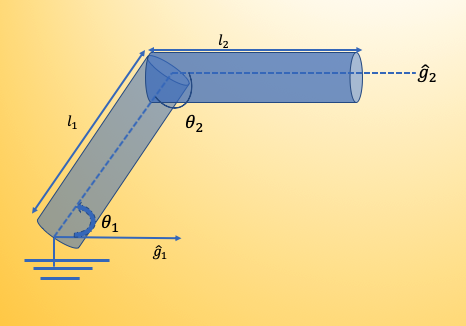
\includegraphics[width=.7\columnwidth]{figures/planar_manip.png}
	\caption{An illustration of the geometric configuration of the planar arm}
	\label{fig:planar_manip}
\end{figure}
%
\begin{subequations}
	\begin{align}
	\homo_1 = l_1 \cos \theta_1 + l_2 \nonumber \\
	%
	\homo_2 = l_1 \sin \theta_1 + l_2 \sin(\theta_1+\theta_2)
	\end{align}
\end{subequations}
% 
and whose first order time derivative yields,
%
\begin{subequations}
	\begin{align}
	\dot{\homo}_1 = -l_1 \dot{\theta}_1 \sin \theta_1  \nonumber \\
	%
	\dot{\homo}_2 = l_1 \dot{\theta}_1 \cos \theta_1 + l_2 (\dot{\theta}_1+\dot{\theta}_2) \cos(\theta_1+\theta_2).
	\end{align}
\end{subequations}
%
Vectorizing, we have
%
\begin{align}
	\left(\begin{array}{c}
		\dot{\homo}_1 \\
		%
		\dot{\homo}_2
	\end{array}\right) = \left(\begin{array}{cc}
	-l_1  \sin \theta_1 & 0 \\
	%
	 l_1  \cos \theta_1 + l_2  \cos(\theta_1+\theta_2) &  l_2 \dot{\theta}_2 \cos(\theta_1+\theta_2)
	\end{array}\right)
	%
	\left(\begin{array}{c}
	\dot{\theta}_1 \\
	%
	\dot{\theta}_2
	\end{array}\right)
\end{align}
% 
so that the velocity of the tip point of the 2R robot arm can be written as 
%
\begin{align}
	v_{tip} = J_1(\theta)\dot{\theta}_1 + J_2(\theta)\dot{\theta}_2.
\end{align}
%
We can always guarantee a tip point velocity as long as the columns of the manipulator Jacobian are not collinear. When collinearity occurs, the robot ends up in a \textit{singular configuration} and the Jacobian loses rank (more on this later on). Formally, we say a manipulator is in a singular configuration when the tip of the robot is unable to move arbitrarily in specific directions.

\subsection{The Manipulability Ellipsoid}
%
We now formally introduce the manipulability ellipsoid of the robot arm. When you start designing robot mechanisms, you would need to understand how arbitrarily changing the position and orientation of the end-effector at the tip of the robot arm is a function of the joint velocities and their positions. 
\begin{definition}
	The quantitative index that defines the set of all end-effector velocities that are realizable by joint velocities under a magnitude constraint (\eg a Euclidean norm  $<=1$) such that \textit{those end-effector velocities are \textbf{large and spherical} as much as possible} is the \textbf{manipulability measure} of the robot.
\end{definition}

The manipulability measures the performance of the arm's kinematics (motions) in order for us to optimize the size of the robot. To illustrate the intuitive mesaning of the manipulability measure, play with the cdf file located on the wolfram cloud at this \href{https://demonstrations.wolfram.com/ManipulabilityEllipsoidOfARobotArm/}{web address}. What happens, when you set all the angles of the robot to zero or $180^\circ$? Notice that the manipulability becomes $0$. Coincidentally, we find that this is a situation that occurs when the robot is at a singularity and the manipulability ellipsoid is at its lowest coverage within the manipulator workspace.

\begin{homework}
	Explain what happens when you adjust the parameters of the robot as follows 
	%
	\begin{itemize}
		\item Keep $\theta_1 = \theta_3 = 0$ and vary $\theta_2$. What do you notice about the size of the ellipsoid? How does it affect the mannipulability measure? 
		%
		\item Keep $\theta_2 = \theta_3 = 0$ and set $\theta_1$ at $\pi/2$. What happens to the shape of the ellipsoid? Report the manipulability measure.
		%
		\item Keep any  two the joints at $180^\circ$ and make the other joint $0^\circ$. What do you notice?
	\end{itemize}
\end{homework}

From the \href{http://scriptedonachip.com/downloads/Videos/manipulability.mp4}{video} of the ellipsoids, we notice that the closer the ellipsoids are in area to a circle, the more the freedom we obtain in being able to move the tip in arbitrary directions.  So we define the \textit{manipulability measure} as 
%
\begin{align}
	\sqrt{\dot{q}_1^2(t)+\dot{q}_2^2(t)+\ldots + \dot{q}_l^2(t)} \le 1
\end{align}
%
which is to say the the bound on the Euclidean norm of all joint angle velocities such that it is less than unity and we define the manipulability ellipsoid as 
%
\begin{align}
	\{ v(t) J^{-T} \cdot J^{-1} \cdot v(t) \le 1, v(t): Rank(J) \}
 \end{align}

\section{The Manipulator Jacobian}

Here, we are concerned with the magnitudes of the joint velocities when the  $\dot{\theta}_i = 1$ and all other joint velocities are $0$. This determines the twist, which we treated in \autoref{chap:rbm}. Particularly, we separate the treatments of the spatial manipulator Jacobian (\ie the the Jacobian where each column of $J$ is a screw axes in the base or a fixed spatial frame, $s$) and the body manipulator Jacobian (\ie the Jacobian where each column of $J$ is a screw axes in the the end-effector frame, $b$).

\subsection{Spatial Jacobian}
%
Consider the general Jacobian of \eqref{eq:jacob_gen}, suppose now that $g_{st} \rightarrow SE(3)$ is a forward kinematic map for the manipulator and the joints traverse a path $\theta(t) \in Q$, so that the end-effector follows a path $\homo_{st}(\theta(t)) \in SE(3)$. The instanteneous spatial velocity of the end-effector would be the set 
%
\begin{align}
	\hat{\eta}^s_{st} = \dot{\homo}_{st}(\theta) \homost^{-1}(\theta)
	\label{eq:spatial_jacob}
\end{align}
%
Applying the chain rule as before (\cf \eqref{eq:jacob_gen}), we have 
%
\begin{align}
	\hat{\eta}^s_{st}  = \sum_{i=1}^{n} \left(\dfrac{\partial \homo_{st}({\theta})}{\partial \theta_i} \dot{\theta}_i \right) \homost^{-1}(\theta) =  \sum_{i=1}^{n} \left( \dfrac{\partial \homo_{st}({\theta})}{\partial \theta_i} \homost^{-1}(\theta) \right) \dot{\theta}_i.
\end{align}
%
In twist coordinates, we write the above as 
%
\begin{align}
		\hat{\eta}^s_{st}  = J_{st}^s(\theta) \dot(\theta)
\end{align}
%
where
%
\[
	J_{st}^s = \left[\left(\dfrac{\partial \homo_{st}({\theta})}{\partial \theta_1} \homost^{-1}\right)^\vee 
							\ldots
						    \left(\dfrac{\partial \homo_{st}({\theta})}{\partial \theta_l} \homost^{-1}\right)^\vee 
							\right]
\]
%
and the $i'th$ joint twist transformed by $e^{\twistmap_1 \theta_1} \ldots e^{\twistmap_{i-1}\theta_{i-1}}$ from the $i'th$ joint in the reference configuration to the current configuration of the manipulator is
%
\[
	\left(\dfrac{\partial \homo_{st}({\theta})}{\partial \theta_1} \homost^{-1}\right)^\vee = \text{Ad}_{\left(e^{\twistmap_1 \theta_1}\ldots e^{\twistmap_{l-1} \theta_{l-1}}\right)}\twistmap_l :\equiv \twistcoord^\prime.
\]
%
It therefore follows that 
%
\begin{align}
	J_{st}^s(\theta) = \left[\twistcoord_1, \twistcoord_2^\prime  \ldots \twistcoord^\prime_l \right]
\end{align}
%
We thus see that the \textit{i'th column of the Jacobian corresponds to the i'th joint twist, transformed to the current manipulator configuration.}

\subsection{The Body Jacobian}
%
In body coordinates, we rewrite \eqref{eq:spatial_jacob} as 
%
\begin{align}
\hat{\eta}^b_{st} = J^b_{st}(\theta)\dot{\theta}
\label{eq:body_jacob}
\end{align}
%
so that 
%
\begin{subequations}
	\begin{align}
	J_{st}^b(\theta) =  \left[\twistcoord_1^\star, \twistcoord_2^\star  \ldots \twistcoord^\star_{l-1} \twistcoord^\star_{l} \right] \\
	%
	\twistcoord_i^\star = \text{Ad}^{-1}_{\left(e^{\twistmap_1 \theta_1}\ldots e^{\twistmap_{l} \theta_{l}}\homost(0)\right)}\twistmap_i
	\end{align}
\end{subequations}
%
where the $\homost(0)$ term allows us the freedom to choose the base frame in order to simplify our calculations (\eg choose $\homost(0) = I$.

Before we close this section, we note the following relations between the two Jacobians:
%
\begin{align}
	J_{st}^s(\theta) = Ad_{\homost(\theta}J_{st}^b(\theta).
\end{align}
%
These spatial and body manipulator Jacobians are useful in finding the instanteneous velocity of the tip point in the end-effector frame. Suppose we let $q^b$ be this tip point in body coordinates, we can find the velocity $v^b$ in the tool frame (body coordinates) as 
%
\begin{align}
	v^b_q = \hat{\eta}_{st}^b q^b = \left(J_{st}^b(\theta) \dot{\theta}\right)^\wedge q^b.
\end{align}
%
The logic above applies in spatial coordinates (\ie the base frame), whereupon we have
%
\begin{align}
v^s_q = \hat{\eta}_{st}^s q^s = \left(J_{st}^s(\theta) \dot{\theta}\right)^\wedge q^s
\end{align}

Notice from \eqref{eq:spatial_jacob} that 
%
\begin{align}
	\dot{\theta}(t) = \left(J_{st}^s(\theta)^{-1} \eta_{st}^s (t) \right)
\end{align}
%
implying that we do not need the inverse kinematics of the manipulator of the robot if we want to move an arm from one end-effector pose to another since we know the relationship between the joint velocities and the end-effector velocity.

\begin{homework}
	Explain how you would go about implementing the last part of the above statement for the planar robot arm of \autoref{fig:planar_manip}.
\end{homework}

\section{Inverse kinematics}
%
We formally define the inverse kinematics problem as follows: given a desired configuration for the end-effector, $\homo_d$, find the joint angles necessary for achieving that configuration. Mathematically, we can think of this as being given a forward kinematic map $\homost: Q \rightarrow SE(3)$, and $\homo_d$, find the desired joint angles by solving 
%
\begin{align}
	\homost(\theta) = \homo_d
\end{align}
%
for some $\theta \in Q$. It is noteworthy to here point out that the IK problem mat have multiple solutions,, a unique solution or no solution at all. It is typical to use numerical optimization approaches to solve these problems in practice. In ROS, there are different IK libraries that are available such as the ones from \textsc{KDL} or 

\begin{example}
	Consider the two-link planar arm of \autoref{fig:ik_ex}. This example is taken from \cite{MurrayBook}. We know the forward kinematics to be 
	%
	\begin{align}
		x = l_1 \cos \theta_1 + l_2 \cos(\theta_1 + \theta_2) \nonumber \\
		%
		y = l_1 \sin \theta_1 + l_2 \sin(\theta_1 + \theta_2).
	\end{align}
	%
	In order to solve for $\theta_1$ and $\theta_2$ given $x$ and $y$, we use polar coordinates to parameterize the geometry (see the right inset). We see that 
	%
	\begin{subequations}
		\begin{align}
			r &= \sqrt{x^2 + y^2} \\
			\theta_2 &= \pi \pm \alpha \\
			\alpha &= \cos^{-1} \frac{l_1^2 + l_2^2- r^2}{2 l_1 l_2}.
		\end{align}
	\end{subequations}
	%
	That is, $\theta_2$ could take on two possible values when $\alpha \neq 0$. The second value of $\theta_2$ is shown by the dashed line, called the ``flipped' solution''. We find $\theta_1$ by solving
	%
	\begin{align}
	\theta_1 = a\tan2(y,x) \pm \beta, \quad \beta = \cos^{-1}\left(\frac{r^2 + l_1^2 - l_2^2}{2 l_1l_2}\right)
	\end{align}
	%
	with the condition that the sign of $\alpha$ must correspond to the one used for $\beta$.
	%
\end{example}


\begin{figure}[tb!]
	\centering
	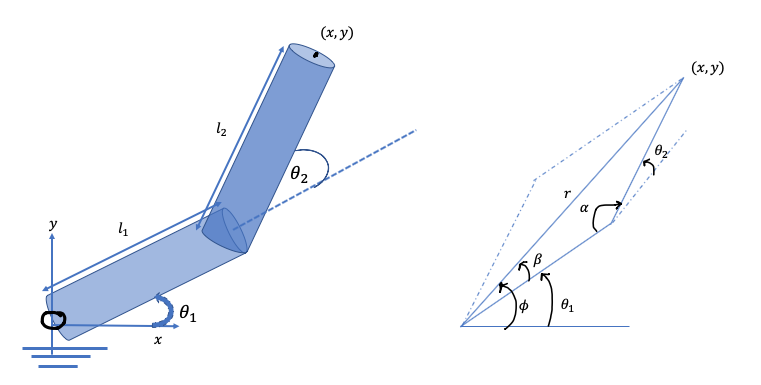
\includegraphics[width=.8\columnwidth]{figures/ik_ex.png}
	\caption{Inverse Kinematics of a two-link planar manipulator}
	\label{fig:ik_ex}
\end{figure}
%%\chapter{Statics and Velocity Kinematics}
\label{chap:statics}

\section{Singularities in Configurations}

\section{The antisymmetric matrix}

\section{Derivation of Rotation Matrices}

\section{The Manipulator Jacobian: Derivation}

\section{Relating the Spatial to Body Jacobian}

\section{Velocities of the tip and tool frames}

\section{Decoupling singularities}

\section{The principle of virtual work}

\section{Manipulability}
%\chapter{Robot Dynamics and Control}
%
At issue in this chapter are the motions of various components of a robot given the forces, torques and momentum that act upon it. In rigid body dynamics, we typically represent these dynamics using nonlinear, second-order differential equations which are a function of the kinematics and kinetics of the robot.  While in principle, we can individually sum the forces and torques acting on an object, in practice, it is easier working with the system's \textit{Lagrangian, a summation of all the mechanical energies of the system}, as this tends to be less prone to error than summing together the Coriolis, centrifugal and inertial forces acting on the robot's links. 

The control problem for robot manipulators requires us knowing the dynamics of the robot. This is sometimes called the \textit{inverse dynamics problem} of a robot manipulator, \ie given the mass matrix, Coriolis forces and torques for all the individual robot joints, find the control law that yields a desired motion in space. Assuming that the model we have found is perfect, the control law is very simple. In practice, a feedback control (and sometimes coupled with a robust control) law needs to be derived to correct unmodeled uncertainties and improve trajectory following~\cite{Ogunmolu18IROS}.

There are two methods of controlling a rigid robot: \textit{joint space control} and \textit{workspace control}. In joint space control, a manipulation or navigation task is converted to a desired trajectory for the joints of a robot. We then find a control law to apply actuator torques to the joints of the robot in order to follow a given trajectory. In workspace control, the dynamics and control problem is changed into the task space of the robot so that trajectory commands are given in the coordinates of the end-effector.

\section{Lagrangian for Mechanical Systems }
%
For a system of $n$ particles obeying Newton's second law of motion, the time rate of change of the particle's momentum is the external force applied on the particle. Suppose $F_i$ is the applied force on the $i^{th}$ particle, $m_i$ is the particle's mass, and $r_i$ is the position, it follows from Newton's law that 
%
\begin{align}
	F_i = m_i r_i \quad r_i \in \bb{R}^3, i = 1, \ldots, n.
	\label{eq:RBD_Newton}
\end{align}
%
We are interested in the material description of the body where the overall degrees of freedom is constrained by the coupling between the individual robots. In the \textit{material description}, we are interested with the body-points as it is treated in analytical dynamics, where it is typical to work with first, second, $\ldots$, $n^{th}$ masses. As such, we write out the constraints which govern the particle's positions as the following holonomic constraint\footnote{
%
If time enters the relation in the equation explicitly, then we have a rheonomic constraint, otherwise, the constraint is called sclerenomic constraint. A particle suspended from a tight rope in 3D space would be an example of a rheonomic constraint with the equation, $(x_1-1)^2  + (x_2 - b)^2 + (x_3-c)^2 - r^2 = 0$, while a particle on a carousel would be a sclerenomically-constrained system. Such a system would be described by the following equation, $x_1 = a \cos(\omega t + \phi); x_2 = a \sin (\omega t + \phi).$}. These are the constraints of position in a system.  
%
\begin{align}
g_i(r_1, \ldots, r_n) = 0, \quad j = 1, \ldots, k.
\label{eq:holonomic}
\end{align} 
%
In general, holonomic constraints are systems whose \dofs can be written in an algebraic relationship where the positions are a direct function of velocities. 

Constraints act on a system of particles through the application of \textit{constraint forces} such that they are forces that are normal to smooth surfaces in $\bb{R}^n$. Suppose we have the basis for the constraint forces (not necessarily orthonormal) as $\Gamma_1, \ldots, \Gamma_k \in \bb{R}^3n$ and $\lambda_j$ are the respective scaling factors for the $j^{th}$ basis elements, then we can write Newton's second law that governs the system of equations as 
%
\begin{align}
	F = \begin{bmatrix}
	m_1 \, I &  & 0 \\
	%
	& \ddots & \\
	%
	0 & & m_n \, I
	\end{bmatrix}
	%
	\begin{bmatrix}
	\ddot{r}_1  \\ \vdots \\ \ddot{r}_n
	\end{bmatrix} +  \sum_{j=1}^{k} \Gamma_j \lambda_j
\end{align}
%
where $\Gamma_j$ for the holonomic constraints of \eqref{eq:holonomic} can be taken as the gradients of $g_j$, essentially the level sets of $g_j(r) = 0$. 
%
While simple, this approach does not scale well to the configuration of the sort of rigid bodies we deal with in robotics. A better approach is to use a smaller set of variables that parameterizes the configuration of the system. For a system of $n$ particles with $k$ constraints, we find a set of $m = 3n -k$ variables $q_1, \ldots , q_m$ and smooth functions $f_1, \ldots, f_n$ such that 
%
\begin{align}
	r_i = f_i(q_1, \ldots, q_m), \quad i = 1, \ldots, n \\
	%
	g_j(r_1, \ldots, r_n) = 0, \quad j = 1, \ldots, k
\end{align}
%
where $q_i$'s are the generalized coordinates of the system, which in the case of robot manipulators is almost always the joint angles.  The forces expressed along the coordinates of the generalized coordinates of position are referred to as \textit{generalized forces}. 

\section{Euler-Lagrange Equations}
%
For a kinetic energy $T$ and a potential energy $V$, the \textit{Lagrangian, $L$}, of the system in generalized coordinates is the difference between the kinetic and potential energy, \ie
%
\begin{align}
L(q, \dot{q}) = T(q, \dot{q}) - V(q).
\label{eq:lagrange}
\end{align}
%
In general, we write the kinetic energy in the form, 
%
\begin{align}
	T(\theta) = \frac{1}{2} \sum_{i = 1}^{n} \sum_{j = 1}^{n}  m_{ij}(\theta) \dot{\theta}_i \dot{\theta}_j = \frac{1}{2} \dot{\theta}^T M(\theta) \dot{\theta}
\end{align}
% 
with $m_{ij}$ being the ($i, j$)th element of the mass matrix $M(\theta)$. 
%
The equations of motion for a rigid body articulated system is of the form
%
\begin{align}
\dfrac{d}{dt}\dfrac{\partial L}{\partial \dot{q}_i} - \dfrac{\partial L}{\partial q_i} = \torque_i, \quad i = 1, \ldots, m
\label{eq:lagrange_compo}
\end{align}
%
where $\torque_i$ is the torque acting on the $i^{th}$ generalized coordinate. Hence, we can explicitly write the dynamics as 
%
\begin{align}
\sum_{j=1}^{n} m_{ij}(\theta) \ddot{\theta}_j + \sum_{j = 1}^{n} \sum_{k = 1}^{n} \Gamma_{ijk}(\theta) \dot{\theta}_j \dot{\theta}_k + \dfrac{\partial V}{\partial \theta_i } = 	\torque_i, \quad i = 1, \ldots, n
\end{align} 
%
with $\Gamma_{ijk}(\theta) $ being the so-called \textbf{Christoffel symbols of the first kind}, defined as, 
%
\begin{align}
	\Gamma_{ijk}(\theta)  = \frac{1}{2}\left(\dfrac{\partial m_{ij}}{\partial \theta_k} + \dfrac{\partial m_{ik}}{\partial \theta_k} - \dfrac{\partial m_{jk}}{\partial \theta_i}.
	\right)
\end{align}
%
Essentially, the Christoffel symbols determine the Coriolis and centripetal terms in the matrix $\coriolis(\theta, \dot{\theta}$ as we shall see shortly and they are by-products of the mass matrix $\massinertia(\theta)$. 
%
Written in matrix form equation, we can write the Euler-Lagrange equation of \eqref{eq:lagrange_compo} as
%
\begin{align}
\dfrac{d}{dt}\dfrac{\partial L}{\partial \dot{q}} - \dfrac{\partial L}{\partial q} = \torque.
\label{eq:lagrange_deri}
\end{align}
%
Equation \eqref{eq:lagrange_deri} is elegant because it reduces the number of coordinates we need to work with from $n$ to $m$ (the number of generalized coordinates) for a system. It can be rewritten as 
% 
\begin{align}
M(\theta) \ddot{\theta} + C(\theta, \dot{\theta}) + N(\theta) = \torque,
\label{eq:lagrange_mat}
\end{align}
%
where we see that the Coriolis and centripetal terms enter the torque equation as quadratic factors for the velocity terms, \ie
%
\begin{align}
	M(\theta) \ddot{\theta} + \dot{\theta}^T \Gamma(\theta) \dot{\theta} + N(\theta) = \torque
\end{align}
%
with $\Gamma_i(\theta)$ being an $n\times n$ matrix with the $(j,k)$the entry as $\Gamma_{ijk}$ and the Coriolis matrix has the $(j,k)$ entry as 
%
\begin{align}
	C_{ij}(\theta, \dot{\theta}) = \sum_{k=1}^{n} \Gamma_{ijk}(\theta) \dot{\theta}_k.
\end{align}
%
Thus for a given robotic mechanical system, finding the dynamics is tantamount to deriving the kinetic and potential energies for the system based on that particular system characteristics. In the next two subsections, we will treat two examples -- a simple pendulum system and the dynamics of a mecanum wheel robot. 

\section{Dynamics of a spherical Pendulum}
%
We now consider the double pendulum of \autoref{fig:double-pendulum} with masses $m_1$ and $m_2$. We would like to find the overall torque of the system based on the Euler-Lagrange system of equations we just derived.
%
\begin{figure}[tb!]
	\centering
	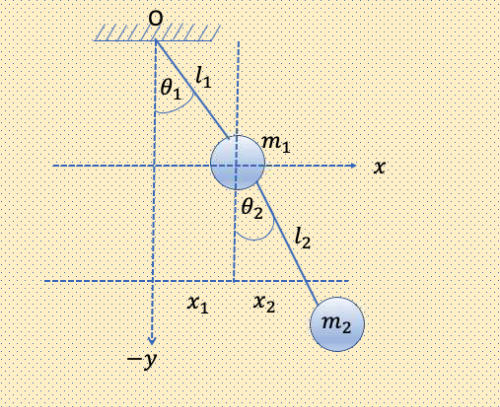
\includegraphics[width=.8\columnwidth]{figures/double-pendulum.png}
	\caption{The double pendulum with configuration is decribed by the angles $\theta_1$ and $\theta_2$.}
	\label{fig:double-pendulum}
\end{figure}
%
First, we write out the position vector of the masses as follows,
%
\begin{align}
	r(\theta_1, \theta_2) = \left(\begin{array}{c|c}
	l_1 \sin \theta_1 & l_1 \sin \theta_1  + l_2 \sin \theta_2
	\\
	-l_1 \cos \theta_1 & -l_1 \cos \theta_1  - l_2 \cos \theta_2
	\end{array}\right)
\end{align}
%
whose time derivative and second time derivative are respectively
%
\begin{align}
	\dot{r} = \left(\begin{array}{c|c}
	\dot{\theta}_1 l_1 \cos \theta_1 & \dot{\theta}_1 l_1 \cos \theta_1  + \dot{\theta}_2 l_2 \cos \theta_2
	\\
	\dot{\theta}_1 l_1 \sin \theta_1 & \dot{\theta}_1 l_1 \sin \theta_1  + \dot{\theta}_2 l_2 \sin \theta_2
	\end{array}\right)
\end{align}
%
and
%
\begin{align}
\ddot{r} = \left(\begin{array}{c|c}
\ddot{\theta}_1 l_1 \cos \theta_1 - \dot{\theta}_1^2 l_1 \sin \theta  & \ddot{\theta}_1 l_1 \cos \theta_1 - \dot{\theta}_1^2 l_1 \sin \theta  + \ddot{\theta}_2 l_2 \cos \theta_1 - \dot{\theta}_2^2 l_2 \sin \theta
\\
\ddot{\theta} l_1  \sin \theta_2 + \dot{\theta}_1^2 l_1 \cos \theta_1  & 
\dot{\theta}_1^2 l_1 \cos \theta_1  + \dot{\theta}_2^2 l_2 \cos \theta_2  + \ddot{\theta}l_1 \sin \theta_1 + \ddot{\theta}_2 l_2 \sin \theta_2 
\end{array}\right)
\end{align}
%
with the associated co-kinetic~\cite{Stramigioli2001} and potential energies
%
\begin{align}
	T = \frac{1}{2} m \|\dot{r}\|^2 = \frac{m_1}{2}l_1^2 \dot{\theta}_1^2 + \frac{m_2}{2}\left(l_1^2 \dot{\theta}_1^2 + l_2^2 \dot{\theta}_2^2 + 2 l_1 l_2 \dot{\theta}_1 \dot{\theta}_2 \cos(\theta_1 - \theta_2) \right)
\end{align}
%
and
%
\begin{align}
	V = g(m_1 \, y_1 + m_2\, y_2) = -m_1gl_1 \cos \theta_1 - m_2 g \left(l_1 \cos \theta_1 + l_2 \cos \theta_2\right)
\end{align}
%
where $g$ in this case denotes the gravitational acceleration.
%
We thus have the Lagrangian of the system as 
%
\begin{align}
	L & = T - V \nonumber \\
	  & = \frac{1}{2}(m_1 + m_2)l_1^2 \dot{\theta}_1^2 + \frac{1}{2}m_2 l_2^2 \dot{\theta}_2^2 + m_2l_1 l_2 \dot{\theta}_1 \dot{\theta}_2 \cos(\theta_1 - \theta_2) + (m_1 + m_2) g l_1 \cos \theta_1 + m_2 g l_2 \cos \theta_2 
\end{align}
%
Now writing the derivatives of the canonical momenta, we have
%
\begin{align}
\dfrac{\partial L}{\partial \dot{r}} &=  (m_1+m_2)l_1^2 \dot{\theta}_1 + m_2 l_2^2 \dot{\theta}_2 + m_2 l_1 l_2 \dot{\theta}_2 \cos(\theta_1 - \theta_2) + m_2 l_1 l_2 (\dot{\theta}_1 + \dot{\theta}_2 )  \cos(\theta_1 - \theta_2) 
% (\dot{\theta}_1 + \dot{\theta}_2) 
\end{align}
%
whereupon, 
%
\begin{align}
	\dfrac{d}{dt}\dfrac{\partial L}{\partial \dot{r}} &=  (m_1+m_2)l_1^2 \ddot{\theta}_1 + m_2 l_1 l_2 \ddot{\theta}_2 \cos(\theta_1 - \theta_2) -  m_2 l_1 l_2 \dot{\theta}_2 \sin(\theta_1 - \theta_2) (\dot{\theta}_1 - \dot{\theta}_2) \nonumber \\
	& \quad + m_2 l_2 \ddot{\theta}_2 + m_2 l_1 l_2 \ddot{\theta}_1 \cos(\theta_1 - \theta_2) - m_2 l_1 l_2 \dot{\theta}_1 \sin (\theta_1 - \theta_2)(\dot{\theta}_1 - \dot{\theta}_2) \\
	%
	\dfrac{d}{dt}\dfrac{\partial L}{\partial \dot{r}} &= (m_1+m_2)l_1^2 \ddot{\theta}_1 + m_2 l_1 l_2 (\ddot{\theta}_1 + \ddot{\theta}_2) \cos(\theta_1 - \theta_2)  + m_2 l_2 \ddot{\theta}_2  \nonumber \\
	& \quad-  m_2 l_1 l_2(\dot{\theta}_1 + \dot{\theta}_2) \sin(\theta_1 - \theta_2) (\dot{\theta}_1 - \dot{\theta}_2) 
\end{align}
and we have for the associated generalized forces
%
\begin{align}
\dfrac{\partial L}{\partial r} &=   - m_2 l_1 l_2  \dot{\theta}_1\dot{\theta}_2 \sin(\theta_1 - \theta_2) - (m_1+m_2)g l_1 \sin \theta_1  + m_2 l_1 l_2  \dot{\theta}_1\dot{\theta}_2 \sin(\theta_1 - \theta_2)  - m_2 g l_2 \sin \theta_2 \nonumber \\
%
\dfrac{\partial L}{\partial r} &= - (m_1+m_2)g l_1 \sin \theta_1- m_2 g l_2 \sin \theta_2
\end{align}
%
Thus, we have the system torque as 
%
\begin{align}
	\torque &= (m_1+m_2)l_1^2 \ddot{\theta}_1 + m_2 l_1 l_2 (\ddot{\theta}_1 + \ddot{\theta}_2) \cos(\theta_1 - \theta_2)  + m_2 l_2 \ddot{\theta}_2  \nonumber \\
	& \quad-  m_2 l_1 l_2(\dot{\theta}_1 + \dot{\theta}_2) \sin(\theta_1 - \theta_2) (\dot{\theta}_1 - \dot{\theta}_2) - (m_1+m_2)g l_1 \sin \theta_1- m_2 g l_2 \sin \theta_2
\end{align}
%
or in matrix form:
%
\begin{align}
	\torque = 
	\begin{bmatrix}
	(m_1+m_2)l_1^2  + m_2 l_1 l_2 \cos(\theta_1 - \theta_2) &  0 \\
	%
	0 & m_2 l_2 + m_2 l_1 l_2 \cos(\theta_1 - \theta_2) 
	\end{bmatrix}
	%
	\begin{bmatrix}
	\ddot{\theta}_1 \\ \ddot{\theta}_2
	\end{bmatrix} + \nonumber \\
	%
	\begin{bmatrix}
	-  m_2 l_1 l_2 \sin(\theta_1 - \theta_2) \\
	%
	-  m_2 l_1 l_2 \sin(\theta_1 - \theta_2)
	\end{bmatrix}^T
	%
	\begin{bmatrix}
	\dot{\theta}_1 \\ \dot{\theta}_2
	\end{bmatrix} 
	%
	+
	\begin{bmatrix}
	- (m_1+m_2)g l_1  \\
	%
	m_2 g l_2 
	\end{bmatrix}^T
	%
	\begin{bmatrix}
		\sin \theta_1 \\
		%
		 \sin \theta_2
	\end{bmatrix}.
\end{align}
%
Therefore, we can write the mass inertia matrix, Coriolis forces and potential energies of the system respectively as, 
%
\begin{align}
	\bm{M} = \begin{bmatrix}
	(m_1+m_2)l_1^2  + m_2 l_1 l_2 \cos(\theta_1 - \theta_2) &  0 \\
	%
	0 & m_2 l_2 + m_2 l_1 l_2 \cos(\theta_1 - \theta_2) 
	\end{bmatrix}
\end{align}
%
\begin{align}
\bm{C} = 	\begin{bmatrix}
-  m_2 l_1 l_2 \sin(\theta_1 - \theta_2) \\
%
-  m_2 l_1 l_2 \sin(\theta_1 - \theta_2)
\end{bmatrix}^T \quad 
%\end{align}
%
\text{ and } \quad 
%
%\begin{align}
	\bm{V} = 	\begin{bmatrix}
	- (m_1+m_2)g l_1  \sin \theta_1  \\
	%
	m_2 g l_2 \sin \theta_2
	\end{bmatrix}
	%
\end{align}
%
so that we may write the equation of motion of the system as 
%
\begin{align}
	\torque - \bm{M}(\theta) + \bm{C}( \theta) + \bm{V}(\theta) = 0.
	\label{eq:torque}
\end{align}
%
The derivation above is very important and will guide us when we start with the control of manipulators and wheeled robots.Equation \eqref{eq:torque} is basically a restatement of Newton's second law of motion, that is the net forces on a rigid body is a summation of the impressed forces (rate of change of the mechanical energy) of the system. The mass matrix is symmetric positive-definite while the $\bm{C}(\theta)$ matrix contains all the Coriolis and centripetal torques, while $V(\theta)$ contains the gravitational torques.

\section{Dynamics of a Mecanum-Wheeled Robot}
%
The example set forth below is from \cite{Ogunmolu18IROS}. You are encouraged to read the paper to get the full context but the subject of importance to us will be introducing the way a rigid body can be controlled. In this case, we will use the gazebo simulation environment to realize torque control of the mobile manipulation system.  Formally,  we consider the KUKA youbot\footnote{\href{https://goo.gl/CYTjvD}{https://goo.gl/CYTjvD}} platform with four mecanum wheels~\cite{mecanum}, capable of spatial $\{x,y\}$ motion, \ie sideways, and forward, and an in-place $\theta$-rotation about the $z$-axis (see Fig. \autoref{fig:mecanum}). It is equipped with a 5-DoF arm, mounted on its base. We use the complete kinematic and dynamic model of the youbot platform, accounting for the wheels' friction and mass, while neglecting the links' masses and their associated inertia forces. %Our goal is to show that while iLQG solves the navigation task with an incomplete model, robust iLQG solves \cmt{the problem faster and better without knowledge of the associated disturbances}. Since the robot moves in the $x-y$ plane, we limit ourselves to the 3-DoF dynamics in Cartesian space.  
The model is derived in spatial (world) coordinates as, $\textit{x}_I = \begin{bmatrix}\textit{x}_1, \textit{x}_2, \textit{x}_3\end{bmatrix}^T \equiv \begin{bmatrix}x_I, y_I, \theta_I\end{bmatrix}^T$, and the local frame of the robot is defined as $\textit{x}_R = \begin{bmatrix}x_R, y_R, \theta_R\end{bmatrix}^T$ (see \autoref{fig:mecanum}).
%
\begin{figure}[tb]
	\centering
	\subfloat[Mecanum Wheels Model]
	{
		\includegraphics[width=0.48\columnwidth]{../../Papers/iDG/IROS2018/figures/robot_mecanum.png}
		\label{fig:mecanum}
	}
	% \caption{Wheels Model.}%
	~ %\qquad
	\subfloat[Robot frames convention	]
	{\includegraphics[width=0.48\columnwidth]{../../Papers/iDG/IROS2018/figures/robot_torques.png}\label{fig:robot_geom}}
	\caption{The KUKA Robot's Geometrical Illustration}
\end{figure}
%
The coordinates of the robot in the world frame are  denoted $\textit{x}_R = \begin{bmatrix}x_R, y_R, \theta_R\end{bmatrix}^T$, where given as the $x_R,\,y_R$ are coordinates of the origin of the robot frame and $\theta_R$ is the relative angle between the  world and robot $x$ axes (see Fig. \autoref{fig:robot_geom}).
%
The torques that govern the robot's motion are obtained from \cite{mecanum}. We run our experiments in the Gazebo physics engine, which has its reference frame defined as $x$ pointing forward, $y$ pointing sideways, and $z$ pointing up. Therefore, our reference frame and robot geometry are as illustrated in Figs \ref{fig:mecanum} and \ref{fig:robot_geom}. Formally, we define the generalized Lagrangian equation of the robot as,
\begin{align}
\bm{M}(\bm{x})\ddot{\bm{x}} + \bm{C}(\bm{x}, \ddot{\bm{x}}) \dot{\bm{x}} + \bm{B}^T \bm{S} \bm{f} = \frac{1}{\bm{r}}\bm{B}^T \torque
\label{eq:inverse_dyn}
\end{align}
%
where $\torque = [\torque_1, \torque_2, \torque_3, \torque_4]$ is the wheel torque vector, $\bm{r}$ is the wheel radius, $\bm{f} = [\bm{f}_1, \bm{f}_2, \bm{f}_3, \bm{f}_4]^T$ is the friction vector, and $\bm{S}$ and $\bm{B}$ map the inverse kinematics, gravity, external forces and robot's angle, $\theta$, %(\ie the angle between the $Y_R$ axis in the  robot local frame's and the  $Y_I$ axis in the world frame)
to each wheel torque; matrices $\bm{B}$ and $\bm{S}$ denote the inertia and coriolis properties of the robot. $\bm{B}$ and $\bm{S}$  are given by,
%
\[
\small
\bm{B} =
\begin{bmatrix}
-(\cos \theta - \sin \theta) & -(\cos \theta + \sin \theta) & -\sqrt{2}l \sin(\zeta) \\
-(\cos \theta + \sin \theta) & (\cos \theta - \sin \theta) &- \sqrt{2}l \sin(\zeta) \\
(\cos \theta - \sin \theta) & (\cos \theta + \sin \theta)  & -\sqrt{2}l \sin(\zeta) \\
(\cos \theta + \sin \theta) & -(\cos \theta - \sin \theta)  & -\sqrt{2}l \sin(\zeta)
\end{bmatrix}
\]
%
\[
\bm{S} = \text{diag} \begin{bmatrix}
sgn(\dot{\phi}_1), \,  sgn(\dot{\phi}_2),  \, sgn(\dot{\phi}_3), \,  sgn(\dot{\phi}_4);
\end{bmatrix}
\]
$\zeta=\pi/4 - \alpha$, $l$ is the mounting distance of the wheels as shown in  Fig. \autoref{fig:mecanum}, and
$\dot{\phi}_i$, is the rotation speed of each wheel about its axis of rotation. We apply the generalized force/torque vector, $F_{i}$, to the base frame of the robot, defined as, %\cite{SpongBook}
\begin{align}
F_{i} = \sum_{j=1}^{4}\left(\torque_j - r \, sgn(\dot{\phi_j}) \, \bm{f}_j\right)\frac{\partial \dot{\phi}_j}{\partial \dot{\bm{x}}_i}, \, i = \{1,2,3\}
\end{align}

%
\begin{figure}[tb!]
	\centering
	\subfloat[Home Position.% The controller is off.
	]{		\includegraphics[height=0.45\columnwidth,width=0.45\columnwidth]{../../Papers/iDG/IROS2018/figures/gazebo_start_state.png}}%
	~ %\qquad
	\subfloat[Goal State.% after repetitive execution of the ILQG algorithm
	]{\includegraphics[height=0.45\columnwidth,width=0.45\columnwidth]{../../Papers/iDG/IROS2018/figures/gazebo_goal.png}}%
	\caption{Goal Navigation Illustration}
	\label{fig:gazebo_sim}
\end{figure}

\begin{homework}
	Using an appropriate controller, command the KUKA robot and arm to move from the center of the maze to the designated goal position shown in \autoref{fig:gazebo_sim}. For this example, students may pull the \textsc{ros docker image} available on the author's docker hub at \href{https://hub.docker.com/r/lakehanne/youbotbuntu14}{https://hub.docker.com/r/lakehanne/youbotbuntu14}. It contains all the inertia masses, Coriolis forces and gazebo package for the youbot robot that you will need for this task. Instructions for loading the environment may be found on this \href{https://github.com/lakehanne/youbot}{github webpage}.
\end{homework}

%\section{Robot Dynamics and the POE Formula}




%\chapter{Motion Planning} 
\label{chap:moplan}

Planning is an important part of robotics. Consider a child (one-year-old) trying to execute a certain simple task such as drinking from a cup of milk. For such a child, this is a very difficult task as they are yet to develop the motor control section of their brain that helps with the hand-eye coordination necessary for the execution of this simple motor task. As such a child evolves, different parts of their brain develops such as the pre-frontal lobes and visual cortex. These, together with innate skills and learning from their environment helps them in eventually mastering the most mundane tasks that aids them throughout life. The way the human brain develops is still a mystery to scientists and if we can understand how the brain works, it would be easy for us to replicate most of these simple automation tasks in real-life. However, given the complexity required for such mastery, researchers have been chipping away at more simpler  ways to plan automation behaviors for a robot. The rest of this course is divided into two phases. In  the first phase, we will deal with works that emerged in the '90's and early 2000's on planning and execution for robots in the world. These tended to leverage subjects that ran the gamut of control theory, information theory and uncertainty quantification. A second parallel in planning and automation that is an evolving field of research has been reinforcement learning and deep reinforcement learning. This area of research involved largely using very deep neural networks (in most cases) as function approximators in encoding future behaviors of a robot by extensively training such a function approximator in a simulator or in a controlled environment.

As the field of studies in these areas are relatively new, there is no certain textbook or mantra for learning what the state-of-the-art is. However, there is a vast array of literature out there in the world on these subjects. Authors of particular interest whose work are very influential are (listed in no particular order of importance) Lydia Kavraki, Steven Lavalle, James Kuffner, Marc Deisenroth, Pieter Abbeel, Ken Goldberg, Sergey Levine and CHelsea Finn among others. In particular, I would refer you to the following text and survey paper as a useful reference throughout the rest of what follows in these notes.
%
\begin{itemize}
	\item LaValle, Steven M. Planning algorithms. Cambridge university press, 2006. \textit{Available at: \href{http://planning.cs.uiuc.edu/}{http://planning.cs.uiuc.edu/}}
	%
	\item Deisenroth, M. P. (2011). A Survey on Policy Search for Robotics. Foundations and Trends in Robotics, 2(1), 1–142. \textit{Available at: \href{https://www.nowpublishers.com/article/Details/ROB-021}{https://www.nowpublishers.com/article/Details/ROB-021}}.
\end{itemize}
%
If you are having trouble downloading any of these materials, please email the instructor for an electronic copy.

\section{Planning: Motion/Trajectory Planning}

In robotics, by planning, we mean the task of automating mechanical or pneumatic systems with the capability for sensing, actuation, and computation abilities. In general, we want to have some sort of algorithm that converts a high-level description of a task to a lower-level one such that we can realize what we want in the real world. \textit{In control systems}, we often design local feedback laws that can act on the dynamics (an encoding of the behavior of the world) of the system so as to realize that which we desire to control. In executing these feedback control laws, we often need a sense of measure of the position and motion of objects in the environment. Typically, this is the sensing problem and it is typically achieved with a vision or tactile or tactile-vision sensor.  Together with the sensed position of the world, we are able to accurately execute an automation task as desired. In \textit{artificial intelligence}, the planning problem is a little loose. Here, the task might involve using discretizing a continuous state space, approximating a complex world with a microcosm of its model.   

Our focus in this chapter is on the algorithmic and the computational issues that arise in planning within several disciplines. In this sentiment, we introduce the notions that enable us to accurately represent a planning algorithm as completely as possible. These are the \textit{states}, \textit{time}, \textit{actions},  \textit{cost} and the \textit{plan}.
%
\begin{definition}[State]
	The state is defined broadly enough to capture all subjective unknowns that might influence future behaviors by a system. For a robot navigating within a grid, for example, the state could be the location of the grid blocks, obstacles and edges within the grid. States can be discrete or continuous. 
\end{definition}
%
\begin{definition}[Time]
The planning problem occurs over a certain (time) horizon. This horizon is often explicitly modeled or implicitly. The important consideration is that a proper sequence must be maintained. Just as a state, time can be dicretized or made continuous.
\end{definition}
%
\begin{definition}[Actions]
	This is a taxonomy that is often used in the AI/computer science robotics world. It is an input that is given to a system that causes it to transition from one state to another state. In control theory literature, you might come across the same term as control/control law.
\end{definition}
%
\begin{definition}[Criterion]
	The criterion is the embodiment of the task's goals. It defines the problem to be solved and provides a measure of how well we are performing towards realizing our objective during the task's execution. There are two functions that we generally concern ourselves about in this regard: 
	\begin{itemize}
	\item \textit{Feasibility}, which is to determine a plan that enables us to reach a goal state, without regard to efficiency
	%
	\item \textit{Optimality}, which is to determine a plan that fulfills certain index or indices of performance such that the end result is arrived at through the most optimal means.
	\end{itemize}
\end{definition}
%
\begin{definition}[Plan]
	A plan imposes a definite strategy or behavior on the decision-making agent. It could be the sequence of actions taken or actions as a function of the state. The plan enables \textit{feedback or reactive plans.}
\end{definition}
%

\section{Planning in Discrete Spaces}
Discrete planning shall involve planning in state spaces where the dimension of the state is finite ot at least infinitely countable \ie, there exists a unique integer that can be assigned to every state. As such, the concepts of representing the state space with a geometric model or complicated differential equations shall not be dealt with herein. We will generally relegate the concepts of uncertainty and avoid methods of representing uncertainty with probability theory.

\subsection{Discrete Feasible Planning}
Suppose we have a state $x \subset X$  where $X$ is a countable finite set.  The events that occur in the world are governed by an action $u$ which acts on a state transition function $f(x, u)$ to generate a new state $\bar{x}$ \ie, 
\[
\bar{x} = f(x, u).
\]
%
Let $U(x)$ be the set of all action spaces for each state $x$ so that the set $U$ of all  possible actions for every state $x \in X$ is defined by 
%
\begin{align}
	U = \bigcup_{x\in X} U(x)
\end{align}
%
while the goal states will be defined by $X_G \subset X$. Our goal will be to find the finite sequence of actions that when applied, transforms the initial state $x_I$ to the goal state in $X_G$. We have the following definition for the model.
%
\begin{algorithm}[tbph!]
	\begin{algorithmic}[1]
		\caption{Discrete Feasible Planning}
		\Require A finite or countably infinite nonempty state space $X$
		%\Function{Discrete Feasible Planning}$X$
		\State For each state $x \in X$, there exists a finite action space $U(x)$
		\State A \textit{state transition function} $f$ produces a state $f(x, u) \in X$ for every $x \in X$ and $u \in U(x)$ so that the \textit{state transition equation} is derived from $f$ as $\bar{x} = f(x,u)$.
		\State An initial state $x_i \in X$.
		\State A goal state $X_g \subset X$
	%	\EndFunction
	\end{algorithmic}
\end{algorithm}

\section{Search Algorithms}
%
Our goal here is to give a skeleton of the common graph search algorithms in robotics. While the questions of computational complexity might be important, this is not our goal here. But rather, we will take a look at the underlings of the popular search algorithms in discrete planning. The state transition graph of such methods are considered to be incrementally given. An important prerequisite in these search paradigms is that the algorithm must be \textit{systematic}. By this, we mean that all visited states must be kept a tab on so that the search does not continue indefinitely. 

For infinite graphs, we may introduce a weaker definition of the \textit{systematic search} requirement. We would require that solutions that exist be found in finite time in such cases; if the solution is however non-existent, we will require the search to run indefinitely. The indefinite search is accomplished by ensuring that as the time taken for exploration of the state space $X$ tends to infinity, every reachable vertex in the graph is explored.
%
\begin{algorithm}[tbph!]
	\begin{algorithmic}[1]
		\caption{Generic Search}
		\Require A priority queue $Q$ for which a sorting function is prescribed
		%\Function{Discrete Feasible Planning}$X$
		\State $Q.add(x_i)$ and mark $x_i$ as visited
		\While{$Q \neq \emptyset$ }
		\State $x\leftarrow Q.getFirst()$ \label{alg:generic-search-lgetfirst}
		\If{$x \in X_g$}
		\State \Return EXIT\_SUCCESS
		\EndIf
		\For {$u\in U(x)$}
		\State $\bar{x} \leftarrow f(x, u)$
		\If{$\bar{x}$ not visited}
		\State Mark $\bar{x}$ as visited
		\State $Q.add(\bar{x})$
		\Else
		\State Resolve duplicate $\bar{x}$
		\EndIf
		\EndFor
		\EndWhile 
		\State \Return EXIT\_FAILURE
	\end{algorithmic}
\label{alg:generic-search}
\end{algorithm}
%
\subsection{General Search Algorithms}
Now consider a general template for the search algorithm where it is required that we transition from an initial state $x_i$ to a final state $x_g$ as depicted in algorithm \ref{alg:generic-search}. At any time during search, three types of states may be encountered viz,
%
\begin{itemize}
	\item \textbf{Unvisited States}: These are states that are not yet visited up until the present time $t$. At the start of the search, this wou;d be every state except $x_i$.
	%
	\item \textbf{Dead States}: These are states that are already visited, and for which every possible next state has also been visited. We say the next state of a state $x$ is a state for which there exists a $u \in U(x)$ such that $\bar{x} = f(x, u)$. Such states are said to be dead because they no longer contribute to the current search procedure.
	%
	\item \textbf{Alive States}: These are states that are already visited, but may have unvisited next states. Originally, the only alive state is $x_i$.
\end{itemize}

The major difference between different search algorithms will be in the type of function that is used to sort the graph $Q$. Typical sorting mechanisms may include one of \textit{first-in first-out (FIFO) policy}, \textit{last-in first-out (LIFO) policy}, \textit{breadth-first search}, or \textit{depth-first search} among others. In a FIFO queue, the state that is the longest in the queue is the one chosen on line \ref{alg:generic-search-lgetfirst}.  The \textit{while} loop is then executed after which it terminates whenever all the states in $Q$ are exhausted. 
%
\chapter{Visual-Inertial Odometry SLAM}

\section{Project Framework}
The goal of this term project is to reinforce everything that we have learned	 in class so far and some more. In particular, I would briefly give an overview of SLAM: the classical and the modern, walk you through some example simple applications and then you will be required to implement a visual inertial odometry SLAM navigation of your robot in an environment of your own choosing (that I will approve). I recommend that you take a look at the stereo-visual inertial odometry example on the \href{https://docs.nvidia.com/isaac/isaac/packages/perception/doc/visual_odometry.html}{isaac webpage} before you send me your proposals.  The Isaac SDK provides a precompiled version of the Elbrus visual odometry library to localize the robot in the world. It does this by continuously analyzing the information from the video stream (in this case the realsense camera sensor). Proposal submissions shall be due in earnest by 23:59:59 on Saturday March 14th, 2020.

\section{Simultaneous Localization and Mapping (SLAM)}

%Since we have a vision-based robot, we will be doing a visual (inertial) odometry-based simultaneous localization and mapping (SLAM). 
By SLAM, we mean the concurrent construction of an environment's model (the map) and the state estimation of the moving robot within it. The robot's state includes the positions, velocities and orientations of different components of the robot per time, although different components may be included such as the bias of the sensors and sensor calibration parameters. The map is used because it can inform of path planning or provide an intuitive visualization for a human operator. The map also allows us to limit the state estimation errors so that dead-reckoning does not drift over time. With the map, the robot is able to reset its localization error by revisiting known areas in a process called \textit{loop-closure}. Sometimes, \textit{a priori} set of landmarks are given to the robot to ease the process of map build-up. For instance, in a manufacturing warehouse where the location of objects and obstacles do not change much, a manually built map can be constructed based on the artificial beacons in the environment. If the robot has access to a GPS, such GPS satellites may be considered as moving beacons at known locations. If such localizations can be reliably carried out, SLAM may not be required\footnote{I promise you that SLAM will be required for the tasks in this term project though.}.  The estimation of the robot's  state  is typically carried out with standard filters such as the extended Kalman filter (ekf).  

SLAM has a common ground with research fields such as computer vision and signal processing. At a higher level, SLAM is a good admixture of geometry, graph theory, optimization, and probabilistic estimation. A SLAM developer has to deal with the practical aspects of integration ranging from sensor calibration, sensor fusion to system integration. It helps to separate SLAM by class into the classical age and the contemporary age. During the classical age, essentially 1986 - 2004, there was the introduction of probabilistic formulations for SLAM, including approaches such as extended Kalman filters, Rao-Blackwellized particle filters and maximum likelihood estimation. With these algorithms, there were the basic challenges connected to efficiency and robust data collection. As such people started looking into ways of conducting better localization and state estimation by merging inertial measurements with visual odometry. This has proven to be really effective in slowly-moving navigation tasks such as MERS robots. % For the remaining weeks in this class, we will need all our programming, mathematical and algorithmic skills in bringing to bear a good SLAM-algorithmic development on our robot.
 
 The goal of SLAM is to build a globally-consistent representation of the environment, leveraging ego-motion measurements and loop closures. Earlier SLAM applications involved odometry being found by integrating wheel encoders. However, the pose estimate from such wheel odometry drifts quickly making the estimate unreliable after a few meters. Recent odometry algorithms are however based on visual and inertial information, and these tend to have very small drift ($< 0.5\%$ of the trajectory length~\cite{SLAMLeonard}). 
 
 In the evolution of robot-based SLAM research, mapping a 2-D indoor environment with a robot that has wheel encoders and a laser scanner with enough accuracy ($< 10$cm) and enough robustness (\eg low failure rate) is almost a solved problem. You can look through the codes available on this page that implements this 2D indoor navigation using the Pioneer P3-DX robot \href{https://github.com/SeRViCE-Lab/p3-dx}{\textit{P3-DX}}. Feel free to play with the simulation using the ROSARIA and ROSARNL libraries as described in the README files on the page. A good industrial example is the \href{https://www.kuka.com/-/media/kuka-downloads/imported/9cb8e311bfd744b4b0eab25ca883f6d3/kuka_navigation_solution_en.pdf}{\textit{Kuka Navigation solution}}. Vision-based SLAM for slowly-moving robots such as the Mars exploration  rovers~\cite{MarsVisualOdometry} can be considered an almost solved problem as well. For example, prior to 2006, NASA's MER were commanded only once per Martian solar day using a prescheduled sequence of precise metrically specified commands such as ``drive forward 2.34 meters, turn in place $0.3567$ radians to the right, drive to location $X, Y$ and take colored pictures of the terrain at location $X,Y, Z$~\cite{leger2005mars}.

%\section{GMapping}
%To successfully be able to navigate a robot in an environment, the grid map of the robot's environment must be built from the ground up. GMapping is a widely used tool in robotics navigation to solve the grid world building and update process. It is based on the OpenSLAM \

\section{Relevant Texts and Materials}

\begin{itemize}
	\item SLAM on the Mars Exploration Rovers: \href{https://onlinelibrary.wiley.com/doi/pdf/10.1002/rob.20184}{Maimone, Mark, Yang Cheng, and Larry Matthies. "Two years of visual odometry on the mars exploration rovers." Journal of Field Robotics 24, no. 3 (2007): 169-186.}
	%
	\item Visual Inertial Localization: \href{http://www.roboticsproceedings.org/rss11/p37.pdf}{Lynen, Simon, Torsten Sattler, Michael Bosse, Joel A. Hesch, Marc Pollefeys, and Roland Siegwart. "Get out of my lab: Large-scale, real-time visual-inertial localization." In Robotics: Science and Systems, vol. 1. 2015.}
	%
	\item SLAM Survey: \href{https://ieeexplore-ieee-org.proxy.library.upenn.edu/stamp/stamp.jsp?tp=&arnumber=7747236}{Cadena, Cesar, Luca Carlone, Henry Carrillo, Yasir Latif, Davide Scaramuzza, José Neira, Ian Reid, and John J. Leonard. "Past, present, and future of simultaneous localization and mapping: Toward the robust-perception age." IEEE Transactions on robotics 32, no. 6 (2016): 1309-1332.}
	%
	\item SLAM Tutorial: Part I. \href{}{Durrant-Whyte, Hugh, and Tim Bailey. "Simultaneous localization and mapping: part I." IEEE robotics \& automation magazine 13, no. 2 (2006): 99-110.}
	%
	\item SLAM Tutorial: Part II. \href{https://ieeexplore.ieee.org/stamp/stamp.jsp?arnumber=1678144}{Bailey, Tim, and Hugh Durrant-Whyte. "Simultaneous localization and mapping (SLAM): Part II." IEEE robotics \& automation magazine 13, no. 3 (2006): 108-117.}
\end{itemize}
%
% ---- Bibliography ----
\providecommand\BIBentryALTinterwordstretchfactor{2.5}
\bibliographystyle{wafr.bst}
%\addbibresource{biblio}
\bibliography{biblio,../../../Papers/SRS/Continuum/biblio,../../../Papers/iDG/IROS2018/root}

\end{document}
